% Options for packages loaded elsewhere
% Options for packages loaded elsewhere
\PassOptionsToPackage{unicode}{hyperref}
\PassOptionsToPackage{hyphens}{url}
\PassOptionsToPackage{dvipsnames,svgnames,x11names}{xcolor}
%
\documentclass[
  letterpaper,
  DIV=11,
  numbers=noendperiod]{scrartcl}
\usepackage{xcolor}
\usepackage{amsmath,amssymb}
\setcounter{secnumdepth}{5}
\usepackage{iftex}
\ifPDFTeX
  \usepackage[T1]{fontenc}
  \usepackage[utf8]{inputenc}
  \usepackage{textcomp} % provide euro and other symbols
\else % if luatex or xetex
  \usepackage{unicode-math} % this also loads fontspec
  \defaultfontfeatures{Scale=MatchLowercase}
  \defaultfontfeatures[\rmfamily]{Ligatures=TeX,Scale=1}
\fi
\usepackage{lmodern}
\ifPDFTeX\else
  % xetex/luatex font selection
\fi
% Use upquote if available, for straight quotes in verbatim environments
\IfFileExists{upquote.sty}{\usepackage{upquote}}{}
\IfFileExists{microtype.sty}{% use microtype if available
  \usepackage[]{microtype}
  \UseMicrotypeSet[protrusion]{basicmath} % disable protrusion for tt fonts
}{}
\makeatletter
\@ifundefined{KOMAClassName}{% if non-KOMA class
  \IfFileExists{parskip.sty}{%
    \usepackage{parskip}
  }{% else
    \setlength{\parindent}{0pt}
    \setlength{\parskip}{6pt plus 2pt minus 1pt}}
}{% if KOMA class
  \KOMAoptions{parskip=half}}
\makeatother
% Make \paragraph and \subparagraph free-standing
\makeatletter
\ifx\paragraph\undefined\else
  \let\oldparagraph\paragraph
  \renewcommand{\paragraph}{
    \@ifstar
      \xxxParagraphStar
      \xxxParagraphNoStar
  }
  \newcommand{\xxxParagraphStar}[1]{\oldparagraph*{#1}\mbox{}}
  \newcommand{\xxxParagraphNoStar}[1]{\oldparagraph{#1}\mbox{}}
\fi
\ifx\subparagraph\undefined\else
  \let\oldsubparagraph\subparagraph
  \renewcommand{\subparagraph}{
    \@ifstar
      \xxxSubParagraphStar
      \xxxSubParagraphNoStar
  }
  \newcommand{\xxxSubParagraphStar}[1]{\oldsubparagraph*{#1}\mbox{}}
  \newcommand{\xxxSubParagraphNoStar}[1]{\oldsubparagraph{#1}\mbox{}}
\fi
\makeatother

\usepackage{color}
\usepackage{fancyvrb}
\newcommand{\VerbBar}{|}
\newcommand{\VERB}{\Verb[commandchars=\\\{\}]}
\DefineVerbatimEnvironment{Highlighting}{Verbatim}{commandchars=\\\{\}}
% Add ',fontsize=\small' for more characters per line
\usepackage{framed}
\definecolor{shadecolor}{RGB}{241,243,245}
\newenvironment{Shaded}{\begin{snugshade}}{\end{snugshade}}
\newcommand{\AlertTok}[1]{\textcolor[rgb]{0.68,0.00,0.00}{#1}}
\newcommand{\AnnotationTok}[1]{\textcolor[rgb]{0.37,0.37,0.37}{#1}}
\newcommand{\AttributeTok}[1]{\textcolor[rgb]{0.40,0.45,0.13}{#1}}
\newcommand{\BaseNTok}[1]{\textcolor[rgb]{0.68,0.00,0.00}{#1}}
\newcommand{\BuiltInTok}[1]{\textcolor[rgb]{0.00,0.23,0.31}{#1}}
\newcommand{\CharTok}[1]{\textcolor[rgb]{0.13,0.47,0.30}{#1}}
\newcommand{\CommentTok}[1]{\textcolor[rgb]{0.37,0.37,0.37}{#1}}
\newcommand{\CommentVarTok}[1]{\textcolor[rgb]{0.37,0.37,0.37}{\textit{#1}}}
\newcommand{\ConstantTok}[1]{\textcolor[rgb]{0.56,0.35,0.01}{#1}}
\newcommand{\ControlFlowTok}[1]{\textcolor[rgb]{0.00,0.23,0.31}{\textbf{#1}}}
\newcommand{\DataTypeTok}[1]{\textcolor[rgb]{0.68,0.00,0.00}{#1}}
\newcommand{\DecValTok}[1]{\textcolor[rgb]{0.68,0.00,0.00}{#1}}
\newcommand{\DocumentationTok}[1]{\textcolor[rgb]{0.37,0.37,0.37}{\textit{#1}}}
\newcommand{\ErrorTok}[1]{\textcolor[rgb]{0.68,0.00,0.00}{#1}}
\newcommand{\ExtensionTok}[1]{\textcolor[rgb]{0.00,0.23,0.31}{#1}}
\newcommand{\FloatTok}[1]{\textcolor[rgb]{0.68,0.00,0.00}{#1}}
\newcommand{\FunctionTok}[1]{\textcolor[rgb]{0.28,0.35,0.67}{#1}}
\newcommand{\ImportTok}[1]{\textcolor[rgb]{0.00,0.46,0.62}{#1}}
\newcommand{\InformationTok}[1]{\textcolor[rgb]{0.37,0.37,0.37}{#1}}
\newcommand{\KeywordTok}[1]{\textcolor[rgb]{0.00,0.23,0.31}{\textbf{#1}}}
\newcommand{\NormalTok}[1]{\textcolor[rgb]{0.00,0.23,0.31}{#1}}
\newcommand{\OperatorTok}[1]{\textcolor[rgb]{0.37,0.37,0.37}{#1}}
\newcommand{\OtherTok}[1]{\textcolor[rgb]{0.00,0.23,0.31}{#1}}
\newcommand{\PreprocessorTok}[1]{\textcolor[rgb]{0.68,0.00,0.00}{#1}}
\newcommand{\RegionMarkerTok}[1]{\textcolor[rgb]{0.00,0.23,0.31}{#1}}
\newcommand{\SpecialCharTok}[1]{\textcolor[rgb]{0.37,0.37,0.37}{#1}}
\newcommand{\SpecialStringTok}[1]{\textcolor[rgb]{0.13,0.47,0.30}{#1}}
\newcommand{\StringTok}[1]{\textcolor[rgb]{0.13,0.47,0.30}{#1}}
\newcommand{\VariableTok}[1]{\textcolor[rgb]{0.07,0.07,0.07}{#1}}
\newcommand{\VerbatimStringTok}[1]{\textcolor[rgb]{0.13,0.47,0.30}{#1}}
\newcommand{\WarningTok}[1]{\textcolor[rgb]{0.37,0.37,0.37}{\textit{#1}}}

\usepackage{longtable,booktabs,array}
\newcounter{none} % for unnumbered tables
\usepackage{calc} % for calculating minipage widths
% Correct order of tables after \paragraph or \subparagraph
\usepackage{etoolbox}
\makeatletter
\patchcmd\longtable{\par}{\if@noskipsec\mbox{}\fi\par}{}{}
\makeatother
% Allow footnotes in longtable head/foot
\IfFileExists{footnotehyper.sty}{\usepackage{footnotehyper}}{\usepackage{footnote}}
\makesavenoteenv{longtable}
\usepackage{graphicx}
\makeatletter
\newsavebox\pandoc@box
\newcommand*\pandocbounded[1]{% scales image to fit in text height/width
  \sbox\pandoc@box{#1}%
  \Gscale@div\@tempa{\textheight}{\dimexpr\ht\pandoc@box+\dp\pandoc@box\relax}%
  \Gscale@div\@tempb{\linewidth}{\wd\pandoc@box}%
  \ifdim\@tempb\p@<\@tempa\p@\let\@tempa\@tempb\fi% select the smaller of both
  \ifdim\@tempa\p@<\p@\scalebox{\@tempa}{\usebox\pandoc@box}%
  \else\usebox{\pandoc@box}%
  \fi%
}
% Set default figure placement to htbp
\def\fps@figure{htbp}
\makeatother





\setlength{\emergencystretch}{3em} % prevent overfull lines

\providecommand{\tightlist}{%
  \setlength{\itemsep}{0pt}\setlength{\parskip}{0pt}}



 


\KOMAoption{captions}{tableheading}
\makeatletter
\@ifpackageloaded{tcolorbox}{}{\usepackage[skins,breakable]{tcolorbox}}
\@ifpackageloaded{fontawesome5}{}{\usepackage{fontawesome5}}
\definecolor{quarto-callout-color}{HTML}{909090}
\definecolor{quarto-callout-note-color}{HTML}{0758E5}
\definecolor{quarto-callout-important-color}{HTML}{CC1914}
\definecolor{quarto-callout-warning-color}{HTML}{EB9113}
\definecolor{quarto-callout-tip-color}{HTML}{00A047}
\definecolor{quarto-callout-caution-color}{HTML}{FC5300}
\definecolor{quarto-callout-color-frame}{HTML}{acacac}
\definecolor{quarto-callout-note-color-frame}{HTML}{4582ec}
\definecolor{quarto-callout-important-color-frame}{HTML}{d9534f}
\definecolor{quarto-callout-warning-color-frame}{HTML}{f0ad4e}
\definecolor{quarto-callout-tip-color-frame}{HTML}{02b875}
\definecolor{quarto-callout-caution-color-frame}{HTML}{fd7e14}
\makeatother
\makeatletter
\@ifpackageloaded{caption}{}{\usepackage{caption}}
\AtBeginDocument{%
\ifdefined\contentsname
  \renewcommand*\contentsname{Table of contents}
\else
  \newcommand\contentsname{Table of contents}
\fi
\ifdefined\listfigurename
  \renewcommand*\listfigurename{List of Figures}
\else
  \newcommand\listfigurename{List of Figures}
\fi
\ifdefined\listtablename
  \renewcommand*\listtablename{List of Tables}
\else
  \newcommand\listtablename{List of Tables}
\fi
\ifdefined\figurename
  \renewcommand*\figurename{Figure}
\else
  \newcommand\figurename{Figure}
\fi
\ifdefined\tablename
  \renewcommand*\tablename{Table}
\else
  \newcommand\tablename{Table}
\fi
}
\@ifpackageloaded{float}{}{\usepackage{float}}
\floatstyle{ruled}
\@ifundefined{c@chapter}{\newfloat{codelisting}{h}{lop}}{\newfloat{codelisting}{h}{lop}[chapter]}
\floatname{codelisting}{Listing}
\newcommand*\listoflistings{\listof{codelisting}{List of Listings}}
\makeatother
\makeatletter
\makeatother
\makeatletter
\@ifpackageloaded{caption}{}{\usepackage{caption}}
\@ifpackageloaded{subcaption}{}{\usepackage{subcaption}}
\makeatother
\usepackage{bookmark}
\IfFileExists{xurl.sty}{\usepackage{xurl}}{} % add URL line breaks if available
\urlstyle{same}
% fallback for those not using the hyperref driver hyperxmp:
\makeatletter
\@ifundefined{xmpquote}{\newcommand{\xmpquote}[1]{#1}}{}
\makeatother
\hypersetup{
  pdftitle={Digital Manufacturing -- Part 1},
  pdfauthor={Paolo Bosetti},
  colorlinks=true,
  linkcolor={blue},
  filecolor={Maroon},
  citecolor={Blue},
  urlcolor={Blue},
  pdfcreator={LaTeX via pandoc}}


\title{Digital Manufacturing -- Part 1}
\usepackage{etoolbox}
\makeatletter
\providecommand{\subtitle}[1]{% add subtitle to \maketitle
  \apptocmd{\@title}{\par {\large #1 \par}}{}{}
}
\makeatother
\subtitle{Digital Manufacturing\\

\includegraphics[width=\linewidth,height=0.3125in,keepaspectratio]{images/by-nc-sa.png}}
\author{Paolo Bosetti}
\date{\emph{Updated:} 14/10/2026}
\begin{document}
\maketitle

\renewcommand*\contentsname{Table of contents}
{
\setcounter{tocdepth}{3}
\tableofcontents
}

\section{Manufacturing systems}\label{manufacturing-systems}

Relevant for the mechatronics point of view

\subsection{Manufacturing systems}\label{manufacturing-systems-1}

\pandocbounded{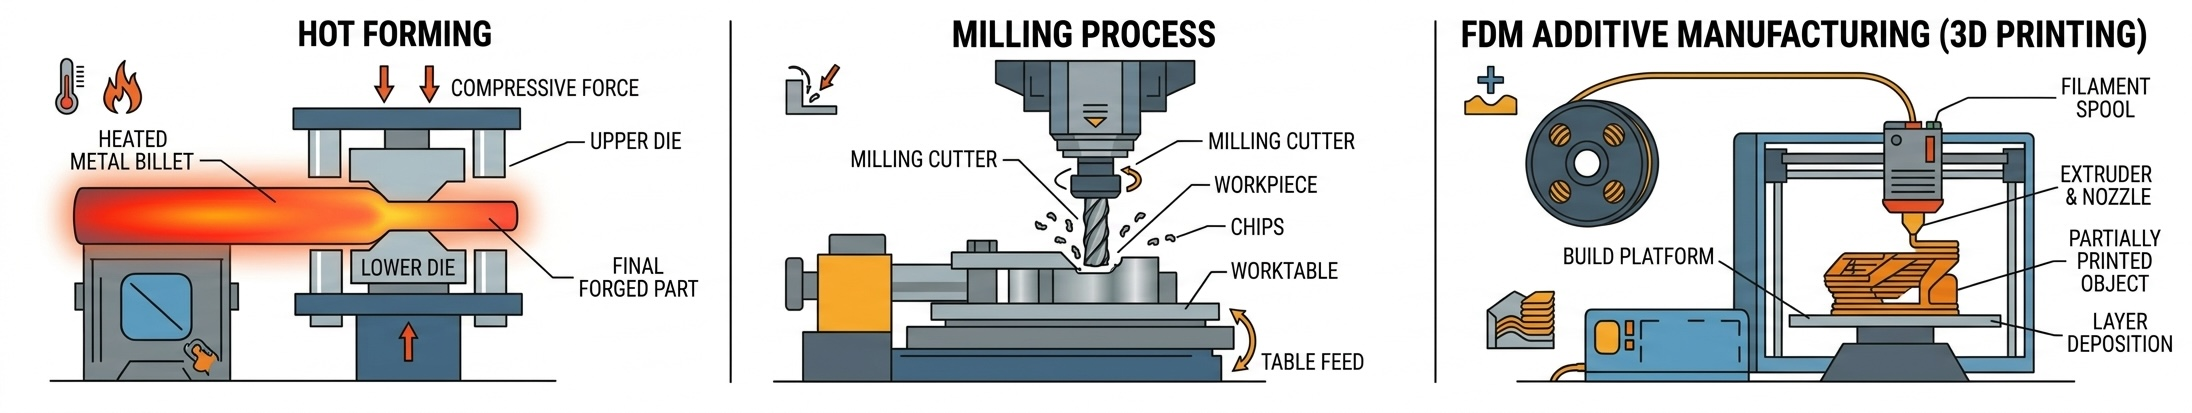
\includegraphics[keepaspectratio]{images-1/technologies.jpg}}

To give shape to a block of raw material (\emph{workpiece}) there are
three possibilities:

\begin{itemize}
\tightlist
\item
  Deform it: \textbf{forming processes} (motion axes: 1+)
\item
  Cut it: material removal (or \textbf{subtractive}) processes (motion
  axes: 2.5+)
\item
  Build on it: \textbf{additive manufacturing} processes (motion axes:
  2.5+)
\end{itemize}

\subsection{Manufacturing systems}\label{manufacturing-systems-2}

\pandocbounded{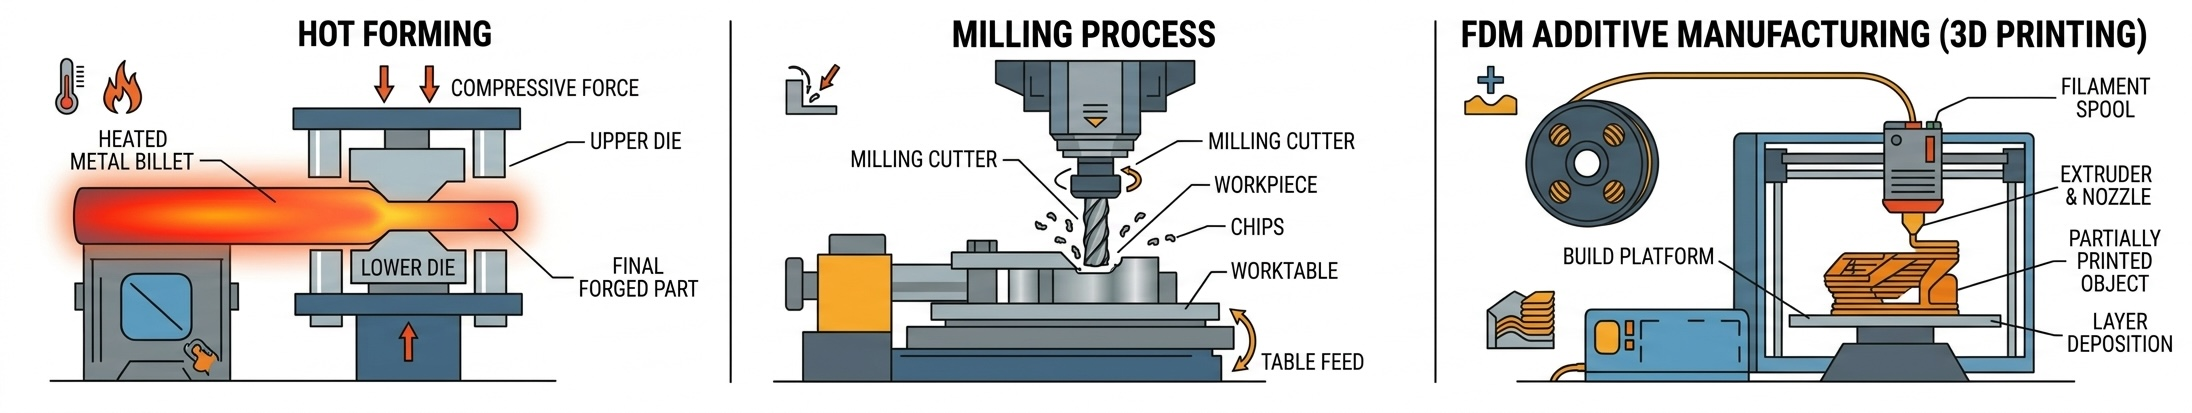
\includegraphics[keepaspectratio]{images-1/technologies.jpg}}

\begin{itemize}
\tightlist
\item
  We skip over forming processes, where motion planning and control is
  trivial (with exceptions!)
\item
  In subtractive and additive manufacturing there is a tool performing
  the process (a mill, a polarized wire, an extruding nozzle, \ldots),
  whose motion is performed by synchronized action of two or more axes,
  typically in cartesian arrangement
\item
  The motion (trajectory and speed) must be planned according to
  geometry and process specifics
\end{itemize}

\subsection{Subtractive Manufacturing: 5-axes
milling}\label{subtractive-manufacturing-5-axes-milling}

\subsection{Additive Manufacturing: 5-axes Direct Laser
Deposition}\label{additive-manufacturing-5-axes-direct-laser-deposition}

\subsection{Reference case:
Turning/Milling}\label{reference-case-turningmilling}

\begin{itemize}
\tightlist
\item
  The majority of products involve machining, either directly, or
  indirectly (dies are machined)
\item
  Machining involves a combination of linear and rotary motions:

  \begin{itemize}
  \tightlist
  \item
    In \textbf{turning}, the workpiece is rotating, the tool is
    displacing
  \item
    In \textbf{drilling and milling} the tool is rotating and there is a
    combined relative displacement between tool and workpiece
  \end{itemize}
\end{itemize}

\begin{tcolorbox}[enhanced jigsaw, arc=.35mm, bottomrule=.15mm, bottomtitle=1mm, breakable, colback=white, colbacktitle=quarto-callout-important-color!10!white, colframe=quarto-callout-important-color-frame, coltitle=black, left=2mm, leftrule=.75mm, opacityback=0, opacitybacktitle=0.6, rightrule=.15mm, title=\textcolor{quarto-callout-important-color}{\faExclamation}\hspace{0.5em}{Important}, titlerule=0mm, toprule=.15mm, toptitle=1mm]

Regardless the process, understanding its physics and the governing
parameters is essential to design the manufacturing system and its
control algorithms

\end{tcolorbox}

\section{The subtractive manufacturing
case}\label{the-subtractive-manufacturing-case}

Material removal processes and their control parameters

\subsection{Machining parameters}\label{machining-parameters}

\begin{itemize}
\tightlist
\item
  Mechanism of \textbf{chip formation} depends

  \begin{itemize}
  \tightlist
  \item
    on the relative speed of tool and workpiece (\textbf{cutting speed})
  \item
    on the \emph{cross section} of removed material
  \end{itemize}
\item
  Cutting speed and cross section (\textbf{tool} parameters) depend in
  turn on trajectory, rotary and translation speeds (\textbf{machining}
  parameters)
\end{itemize}

\subsection{Turning}\label{turning}

Machining parameters to be calculated are \textbf{spindle speed},
\textbf{feed rate}, and \textbf{spindle power}:

\[
\begin{aligned}
\text{Rotational speed:}\quad & N = \frac{v}{\pi D_0} \\
\text{Diameter:}\quad & D_f = D_0 - 2d \\
\text{Feed rate:}\quad & f = N f_r \\
\text{Machining time:}\quad & T_m = \frac{L}{f} = \frac{\pi D_0 L}{f_r v} \\
\text{Material Removal Rate:}\quad & MRR = v f_r d
\end{aligned}
\]

\begin{center}
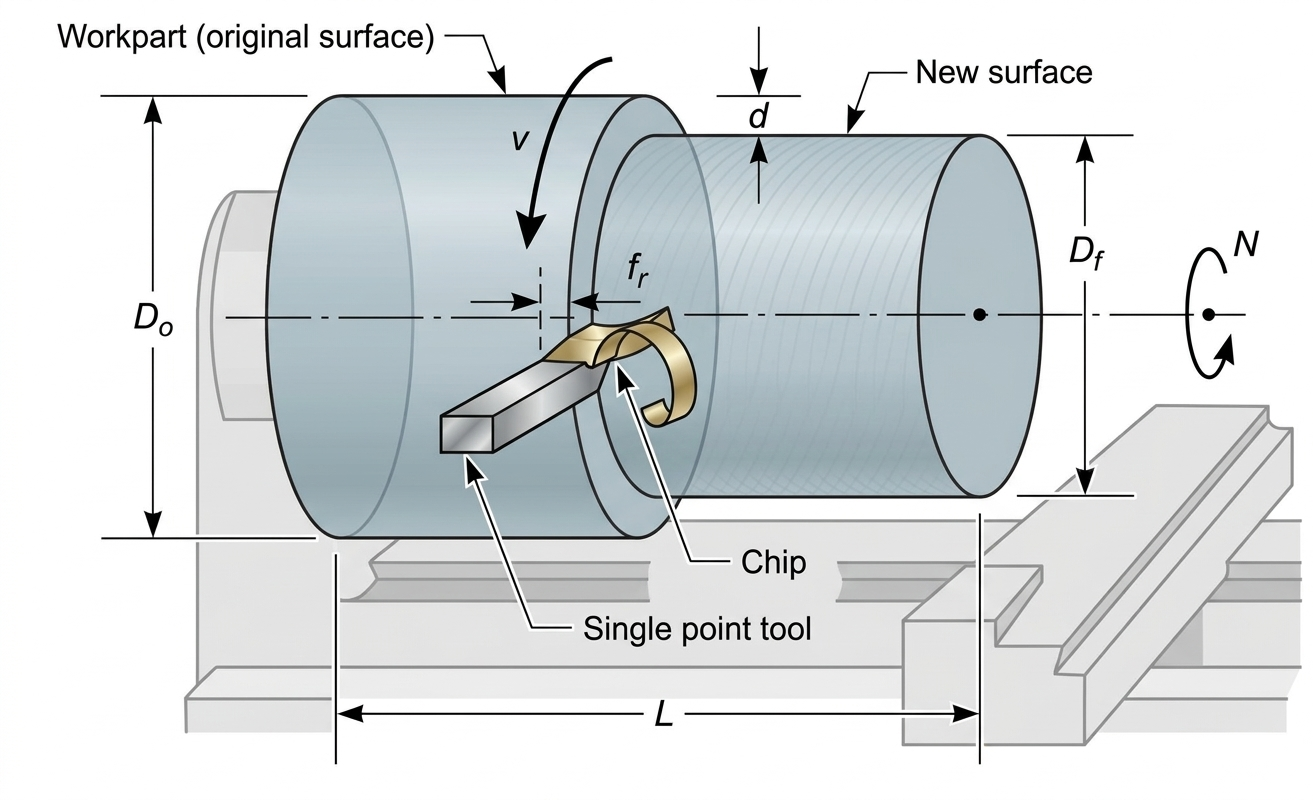
\includegraphics[width=1\linewidth,height=\textheight,keepaspectratio]{images-1/turning.jpg}
\end{center}

\subsection{Drilling}\label{drilling}

Machining parameters to be calculated are \textbf{spindle speed},
\textbf{feed rate}, and \textbf{spindle power}:

\[
\begin{aligned}
N &= \frac{v}{\pi D} \\
f &= N f_r \\
T_m &= \frac{t + A}{f} \\
A &= \frac{D}{2}\tan\left(\frac{\pi - \theta}{2}\right) \\
MRR &= \frac{\pi D^2 f}{4}
\end{aligned}
\]

\begin{center}
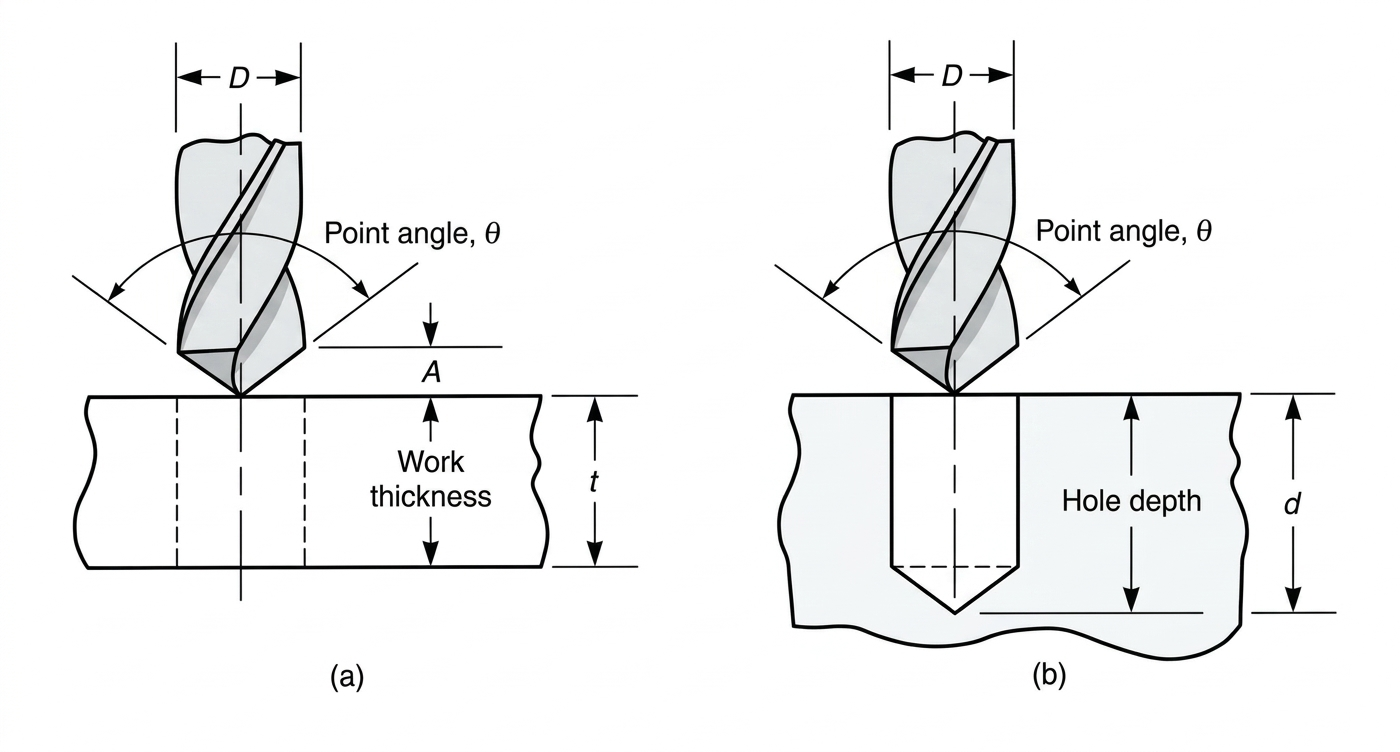
\includegraphics[width=1\linewidth,height=\textheight,keepaspectratio]{images-1/drilling.jpg}
\end{center}

\subsection{Milling}\label{milling}

Machining parameters to be calculated are \textbf{spindle speed},
\textbf{feed rate}, and \textbf{spindle power}. There are three types of
milling:

\begin{center}
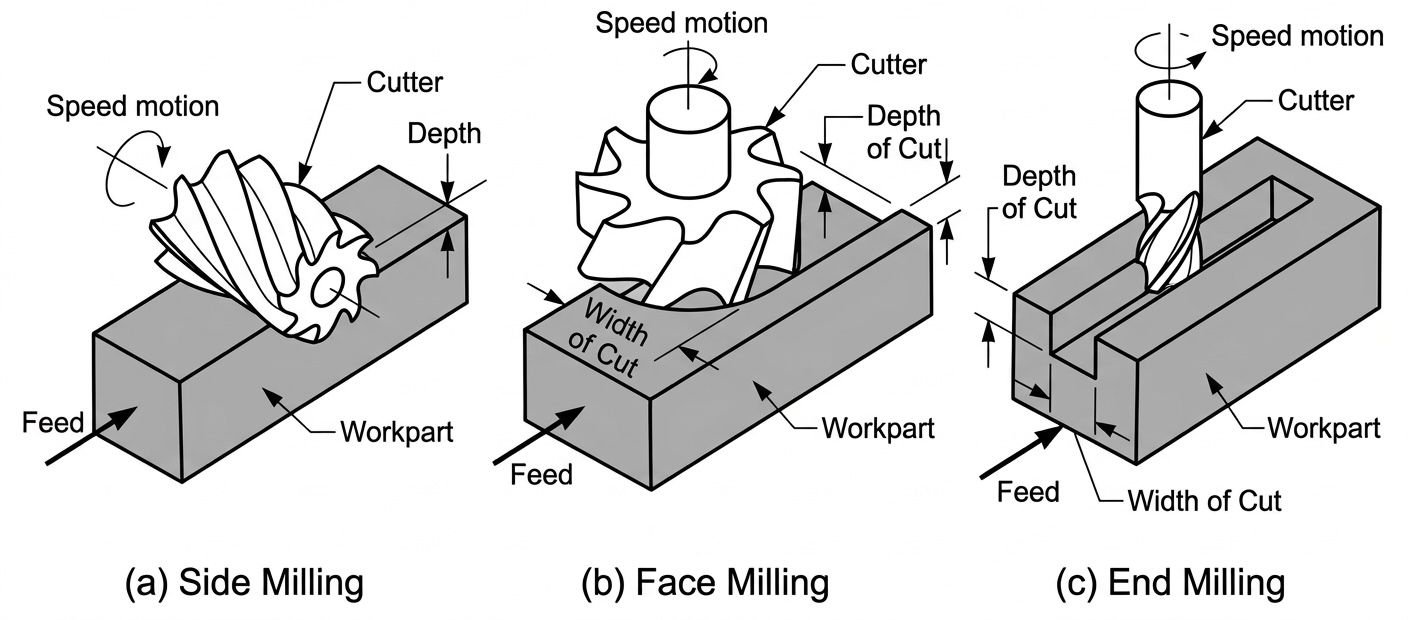
\includegraphics[width=\linewidth,height=4.16667in,keepaspectratio]{images-1/milling.jpg}
\end{center}

\subsection{Milling}\label{milling-1}

\[
\begin{aligned}
N &= \frac{v}{\pi D} \\
f &= N f_z z \\
MRR &= w d f \\
A &= \begin{cases} \sqrt{d(D-d)} & \text{side milling} \\ \sqrt{w(D-w)} & \text{face/end milling} \end{cases} \\
T_m &= \begin{cases} (L + A)/f & \text{side milling} \\ (L + 2A)/f & \text{face/end milling} \end{cases}
\end{aligned}
\]

\begin{center}
\pandocbounded{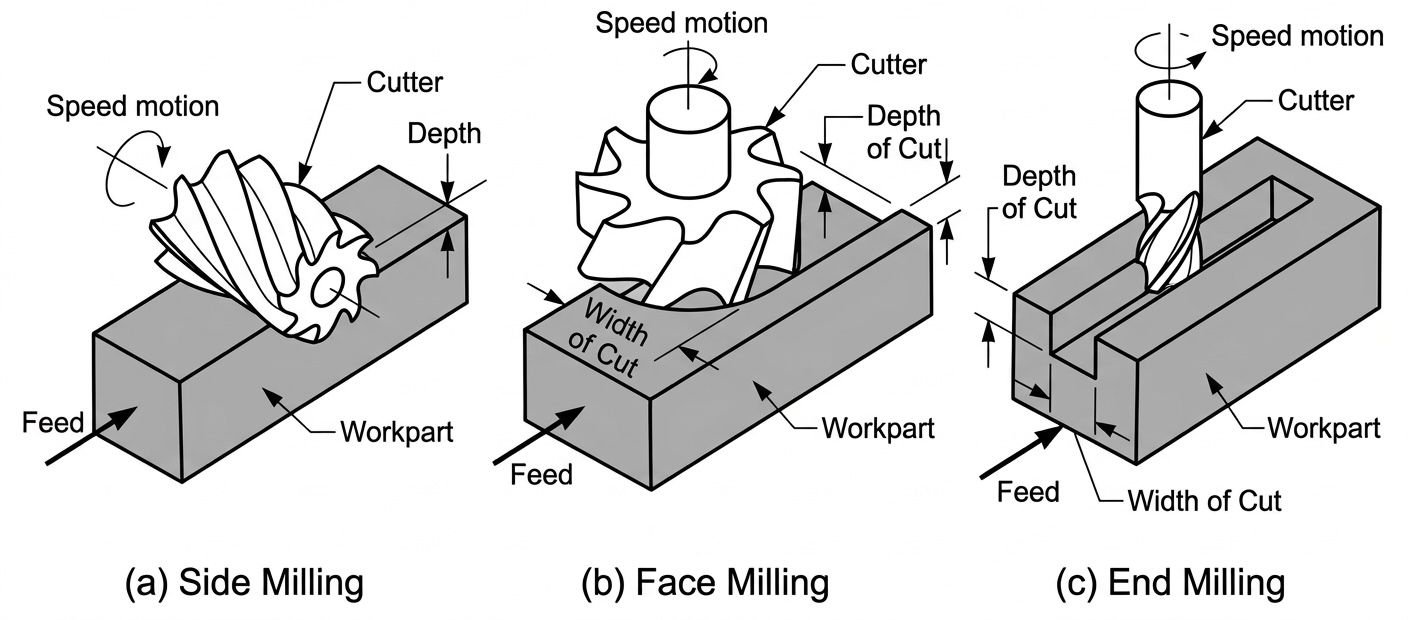
\includegraphics[keepaspectratio]{images-1/milling.jpg}}
\end{center}

\subsection{Shopfloor formulas}\label{shopfloor-formulas}

{\def\LTcaptype{none} % do not increment counter
\begin{longtable}[]{@{}
  >{\raggedright\arraybackslash}p{(\linewidth - 6\tabcolsep) * \real{0.2500}}
  >{\centering\arraybackslash}p{(\linewidth - 6\tabcolsep) * \real{0.2500}}
  >{\centering\arraybackslash}p{(\linewidth - 6\tabcolsep) * \real{0.2500}}
  >{\centering\arraybackslash}p{(\linewidth - 6\tabcolsep) * \real{0.2500}}@{}}
\toprule\noalign{}
\begin{minipage}[b]{\linewidth}\raggedright
Parameter
\end{minipage} & \begin{minipage}[b]{\linewidth}\centering
Turning
\end{minipage} & \begin{minipage}[b]{\linewidth}\centering
Milling
\end{minipage} & \begin{minipage}[b]{\linewidth}\centering
Drilling
\end{minipage} \\
\midrule\noalign{}
\endhead
\bottomrule\noalign{}
\endlastfoot
\(v\) (m/min) & \(v = \pi D_0 N\) & \(v = \pi D N\) & \(v = \pi D N\) \\
\(N\) (1/s) & \(N = \dfrac{v}{\pi D_0}\) & \(N = \dfrac{v}{\pi D}\) &
\(N = \dfrac{v}{\pi D}\) \\
\(f\) (mm/min) & \(f = f_r N\) & \(f = z f_z N\) & \(f = f_r N\) \\
\(f_{z,r}\) (mm) & \emph{Feed per tooth (zahn) or per revolution} & & \\
\(T\) (s) & \(T_m = L/f\) & \(T_m = (L + kA)/f\) & \(T_m = L/f\) \\
\(MRR\) (mm³/min) & \(MRR = d f_r v\) & \(MRR = w d f\) &
\(MRR = \dfrac{\pi D^2}{4} f\) \\
\(P\) (kW) & \(P = MRR\, p_s\) & \(P = MRR\, p_s\) &
\(P = MRR\, p_s\) \\
\(P_e\) (kW) & \(P_e = \dfrac{MRR\, p_s}{\eta}\) &
\(P_e = \dfrac{MRR\, p_s}{\eta}\) & \(P_e = \dfrac{MRR\, p_s}{\eta}\) \\
\end{longtable}
}

\subsection{Example}\label{example}

We have to set up a milling process on Aluminum, which has
\(p_s = 12.56\) W min/cm³

The tool manufacturer suggests \(v = 1000\) m/min and \(f_z = 0.1\)
mm/tooth

The mill has a diameter of \(30\) mm and does face milling with
\textbf{full overlapping}, has \(3\) teeth and removes a layer of \(2\)
mm

\[
\begin{aligned}
N &= \frac{v}{\pi D} = \frac{1000\ \text{m/min}}{\pi\, 30\ \text{mm}} = 10610\ \text{rpm} \\
f &= f_z z N = 0.1\ \text{mm} \cdot 3 \cdot 10610\ \text{rpm} = 3183\ \text{mm/min} \\
MRR &= w d f = 30\ \text{mm} \cdot 2\ \text{mm} \cdot 3183\ \text{mm/min} = 190980\ \text{mm}^3/\text{min} \\
P &= MRR\, p_s = 190.98\ \text{cm}^3/\text{min} \cdot 12.56\ \text{W min/cm}^3 \simeq 2.4\ \text{kW}
\end{aligned}
\]

\begin{tcolorbox}[enhanced jigsaw, arc=.35mm, bottomrule=.15mm, bottomtitle=1mm, breakable, colback=white, colbacktitle=quarto-callout-note-color!10!white, colframe=quarto-callout-note-color-frame, coltitle=black, left=2mm, leftrule=.75mm, opacityback=0, opacitybacktitle=0.6, rightrule=.15mm, title=\textcolor{quarto-callout-note-color}{\faInfo}\hspace{0.5em}{Note}, titlerule=0mm, toprule=.15mm, toptitle=1mm]

The machinist must always ensure that the required maximum power does
not exceed that available at the spindle. If not, some of the machining
parameters must be reduced (usually \(d\) and or \(w\))

\end{tcolorbox}

\subsection{Cutting Economics}\label{cutting-economics}

The cost of machining depends on:

\begin{itemize}
\tightlist
\item
  \textbf{labor:} hourly cost of trained personnel
\item
  \textbf{machinery:} purchase cost / machine life
\item
  \textbf{raw material:} cost of initial workpiece
\item
  \textbf{consumables:} tools, cutting fluids, disposable fixtures
\end{itemize}

Some costs depend on process parameters (mainly cutting speed)

\subsection{Tool wear}\label{tool-wear}

\begin{center}
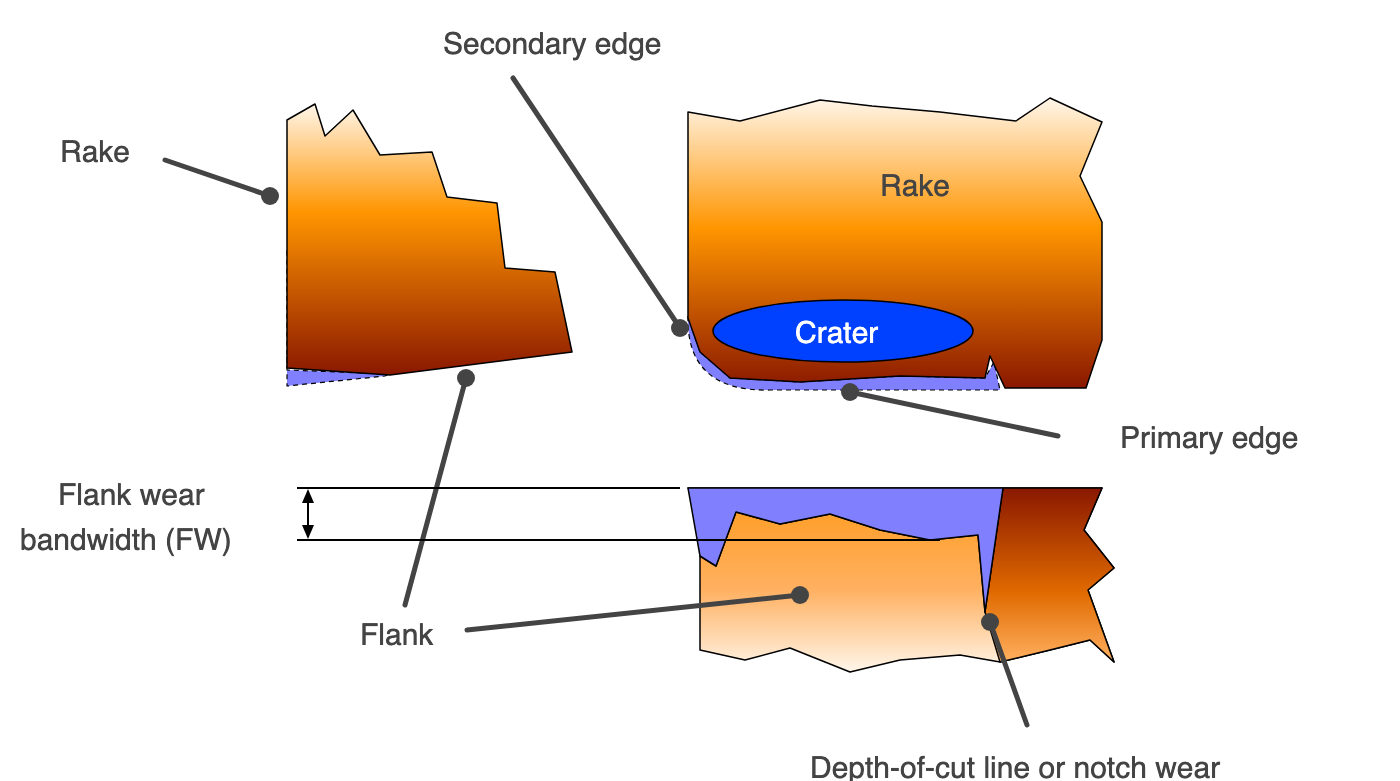
\includegraphics[width=\linewidth,height=5.20833in,keepaspectratio]{images-1/tool-wear.png}
\end{center}

\subsection{Tool wear}\label{tool-wear-1}

Tools are subject to \textbf{wear}. It can affect two parts of the tool:

\begin{itemize}
\tightlist
\item
  the {flank}: it changes the geometry of the tool where it contacts the
  workpiece, so it progressively affects surface quality and dimensional
  accuracy
\item
  the {rake face}: it changes the geometry where the tool contacts the
  chip: it has no effect on the workpiece, but in the long run it
  weakens the tool and causes it to break
\end{itemize}

If the tool and the cutting parameters are chosen correctly, flank wear
occurs before rake face wear

The wear law was formulated by Taylor: \(VT^n=K\), where:

\begin{itemize}
\tightlist
\item
  \(V\) is the cutting speed
\item
  \(T\) is the tool life
\item
  \(n\) and \(K\) are material constants; \(K\) also depends on the
  \textbf{end-of-life criterion} (application specific)
\end{itemize}

\subsection{Taylor's law}\label{taylors-law}

\(VT^n=K \rightarrow \log(V) - n\log(T) = \log(K) \rightarrow \log(T) = \frac{1}{n}\log(V) - \frac{1}{n}\log(K)\)

\subsection{Productivity optimization}\label{productivity-optimization}

The costs of machining production are related to:

\begin{itemize}
\tightlist
\item
  investments and \emph{overhead} ({fixed})
\item
  labor and raw materials ({variable})
\item
  cost per piece ({variable})
\end{itemize}

Costs are dependent variables. The process parameters are
\textbf{independent parameters}

\begin{tcolorbox}[enhanced jigsaw, arc=.35mm, bottomrule=.15mm, bottomtitle=1mm, breakable, colback=white, colbacktitle=quarto-callout-important-color!10!white, colframe=quarto-callout-important-color-frame, coltitle=black, left=2mm, leftrule=.75mm, opacityback=0, opacitybacktitle=0.6, rightrule=.15mm, title=\textcolor{quarto-callout-important-color}{\faExclamation}\hspace{0.5em}{Important}, titlerule=0mm, toprule=.15mm, toptitle=1mm]

We can ask whether there are process conditions that {maximize}
productivity and/or {minimize} costs

\end{tcolorbox}

\subsection{Productivity optimization ---
Turning}\label{productivity-optimization-turning}

{\def\LTcaptype{none} % do not increment counter
\begin{longtable}[]{@{}ll@{}}
\toprule\noalign{}
Symbol & Meaning \\
\midrule\noalign{}
\endhead
\bottomrule\noalign{}
\endlastfoot
\(C_p\) & Cost per piece \\
\(C_m\) & Machining cost \\
\(C_s\) & Setup cost \\
\(C_l\) & Loading cost \\
\(C_t\) & Tooling cost \\
\(L\) & Labor cost \\
\(O\) & Overhead \\
\end{longtable}
}

In \textbf{turning}: \[
T_m = \frac{L}{fN}=\frac{\pi LD}{fV} \\
N_p = \frac{T}{T_m} = \frac{fK^{1/n}}{\pi LDV^{1/n-1}}
\]

\begin{align}
C_p &= C_m + C_s + C_l + C_t \\
C_m &= T_m(L_m + O_m) \\
C_l &= T_l(L_m + O_m) \\
C_t &= \frac{1}{N_p}\left[T_c(L_m+O_m) + T_g(L_g+O_g) + D_c\right] = \frac{C_{t0}}{N_p} \\
T_p &= T_{s,l} + T_m + \frac{C_{t0}}{N_p}
\end{align}

\begin{tcolorbox}[enhanced jigsaw, arc=.35mm, bottomrule=.15mm, bottomtitle=1mm, breakable, colback=white, colbacktitle=quarto-callout-note-color!10!white, colframe=quarto-callout-note-color-frame, coltitle=black, left=2mm, leftrule=.75mm, opacityback=0, opacitybacktitle=0.6, rightrule=.15mm, title=\textcolor{quarto-callout-note-color}{\faInfo}\hspace{0.5em}{Note}, titlerule=0mm, toprule=.15mm, toptitle=1mm]

We have \(C_p=C_p(V)\) and \(T_p = T_p(V)\), so we can differentiate
both to identify an optimal condition

\end{tcolorbox}

\subsection{Productivity optimization ---
Turning}\label{productivity-optimization-turning-1}

\textbf{Costs}: \begin{align}
\frac{\partial C_p}{\partial V} &= 0 \\
V_{o,c} &= \frac{K(L_m+O_m)^n}{[(1/n-1)C_{t0}]^n} \\
T_{o,c} &= (1/n -1)\frac{C_{t0}}{L_m+O_m}
\end{align}

\textbf{Times}: \begin{align}
\frac{\partial T_p}{\partial V} &= 0 \\
V_{o,t} &= \frac{K}{[(1/n-1)T_c]^n} \\
T_{0,t} &= (1/n -1)T_c
\end{align}

\begin{tcolorbox}[enhanced jigsaw, arc=.35mm, bottomrule=.15mm, bottomtitle=1mm, breakable, colback=white, colbacktitle=quarto-callout-note-color!10!white, colframe=quarto-callout-note-color-frame, coltitle=black, left=2mm, leftrule=.75mm, opacityback=0, opacitybacktitle=0.6, rightrule=.15mm, title=\textcolor{quarto-callout-note-color}{\faInfo}\hspace{0.5em}{Note}, titlerule=0mm, toprule=.15mm, toptitle=1mm]

What do we optimize? Costs or times?

\end{tcolorbox}

\subsection{Productivity optimization ---
Turning}\label{productivity-optimization-turning-2}

\begin{itemize}
\tightlist
\item
  The optimal cutting speed \(V_{o,c}\) corresponds to maximum economic
  efficiency
\item
  However, when there are \textbf{penalties for delays} it may be worth
  producing at \(V_{o,t}\), because it is the speed that
  \textbf{maximizes productivity}
\item
  So, \(V\) shall be normally set to \(V_{o,c}\), increasing it up to
  (but not above) \(V_{o,t}\) if there are penalties for delays
\end{itemize}

\subsection{Limits of analytical process
models}\label{limits-of-analytical-process-models}

\subsubsection{Orthogonal cutting}\label{orthogonal-cutting}

\begin{itemize}
\tightlist
\item
  Orthogonal cutting \textbf{rarely applies}. In most real machining
  operations chip formation is inherently 3-D
\item
  The chip formation model is idealized. In reality:

  \begin{itemize}
  \tightlist
  \item
    the cutting edge is never perfectly sharp
  \item
    the shear plane does not have zero thickness
  \item
    deformation does not occur only on the shear plane, but also on the
    machined surface in contact with the cutting edge and between chip
    and tool
  \end{itemize}
\item
  The stress and strain field cannot be computed analytically
\item
  There is no reliable \textbf{thermal model} that accounts for friction
  and plastic deformation as heat sources
\item
  The strain rates involved \(\dot\gamma\) are extreme: this makes it
  very difficult to identify the plastic properties of the material
  under similar conditions
\end{itemize}

\subsection{Limits of analytical process
models}\label{limits-of-analytical-process-models-1}

\subsubsection{Taylor's law}\label{taylors-law-1}

\begin{itemize}
\tightlist
\item
  It is an \textbf{empirical model}, i.e., it has no physical basis but
  rests on observation alone, so it cannot be calibrated from
  measurements of material properties
\item
  It is an approximate law: more complete empirical laws exist in the
  form \(VT^nd^xf^y=K\), which account for other process parameters that
  have a much smaller influence than \(V\) but still affect tool life
\item
  It is \textbf{expensive} to calibrate:

  \begin{itemize}
  \tightlist
  \item
    the experimental procedure is necessarily slow and costly
  \item
    \(n\) depends on the workpiece material and on the tool material
  \item
    \(K\) depends on the \textbf{end-of-life criterion}, so it is
    user-specific (i.e., it cannot be found in tables)
  \end{itemize}
\item
  Even the more complete laws do not account for factors such as
  \textbf{lubrication and cooling}
\end{itemize}

\subsection{Economic optimization}\label{economic-optimization}

\begin{itemize}
\tightlist
\item
  The analysis above depends on being able to \textbf{express \(T_m(V)\)
  analytically}

  \begin{itemize}
  \tightlist
  \item
    This is possible \textbf{only for elementary operations} (e.g.,
    cylindrical turning). For more complex operations the relation can
    only be computed point by point by simulating the process (via CAM
    or CNC functions, which entails \textbf{considerable time and cost})
  \item
    It relies on the availability of a validated and reliable wear law
  \item
    It is worthwhile only for large and very large batches (economy of
    scale)
  \end{itemize}
\end{itemize}

\section{Machine tools}\label{machine-tools}

\begin{figure}[H]

{\centering 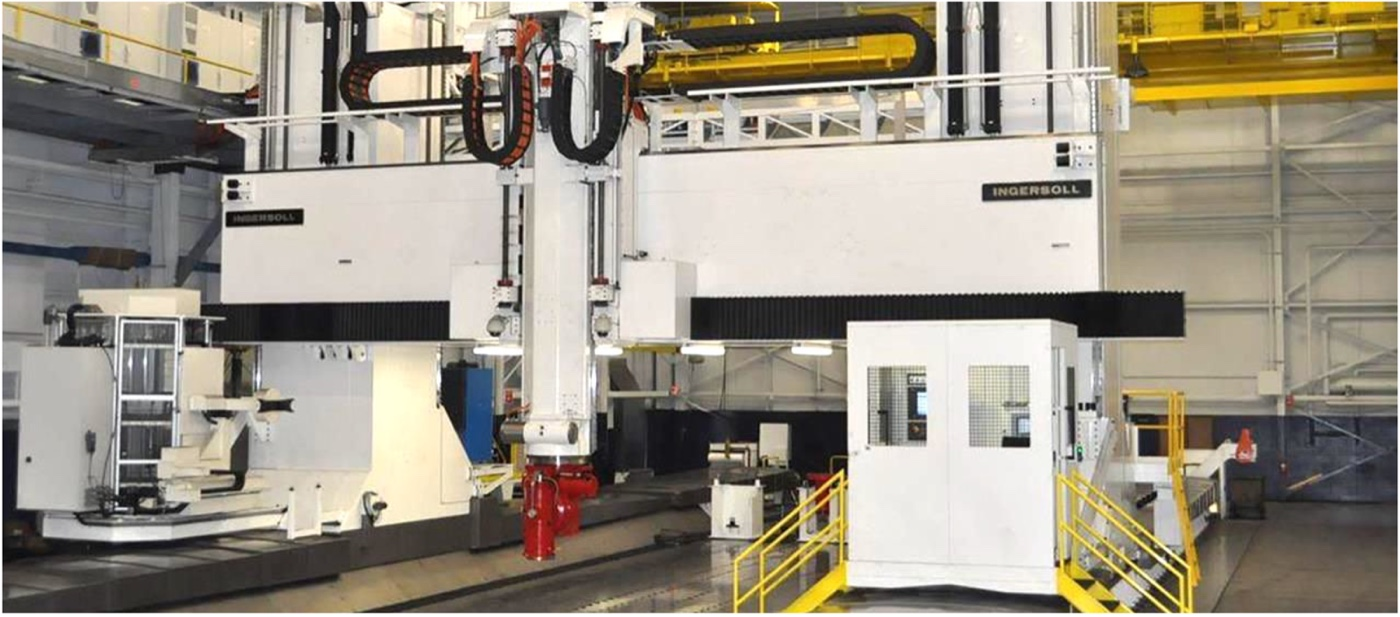
\includegraphics[width=\linewidth,height=3.33333in,keepaspectratio]{images/gantry-mill.jpg}

}

\caption{A gantry-type, large milling center}

\end{figure}%

\subsection{Types of Lathes}\label{types-of-lathes}

\begin{itemize}
\tightlist
\item
  Parallel or engine lathe
\item
  CNC lathe

  \begin{itemize}
  \tightlist
  \item
    Horizontal spindle

    \begin{itemize}
    \tightlist
    \item
      single spindle
    \item
      multiple spindle
    \end{itemize}
  \item
    Vertical spindle
  \item
    Sliding headstock (\emph{fantina mobile})
  \end{itemize}
\end{itemize}

\begin{center}
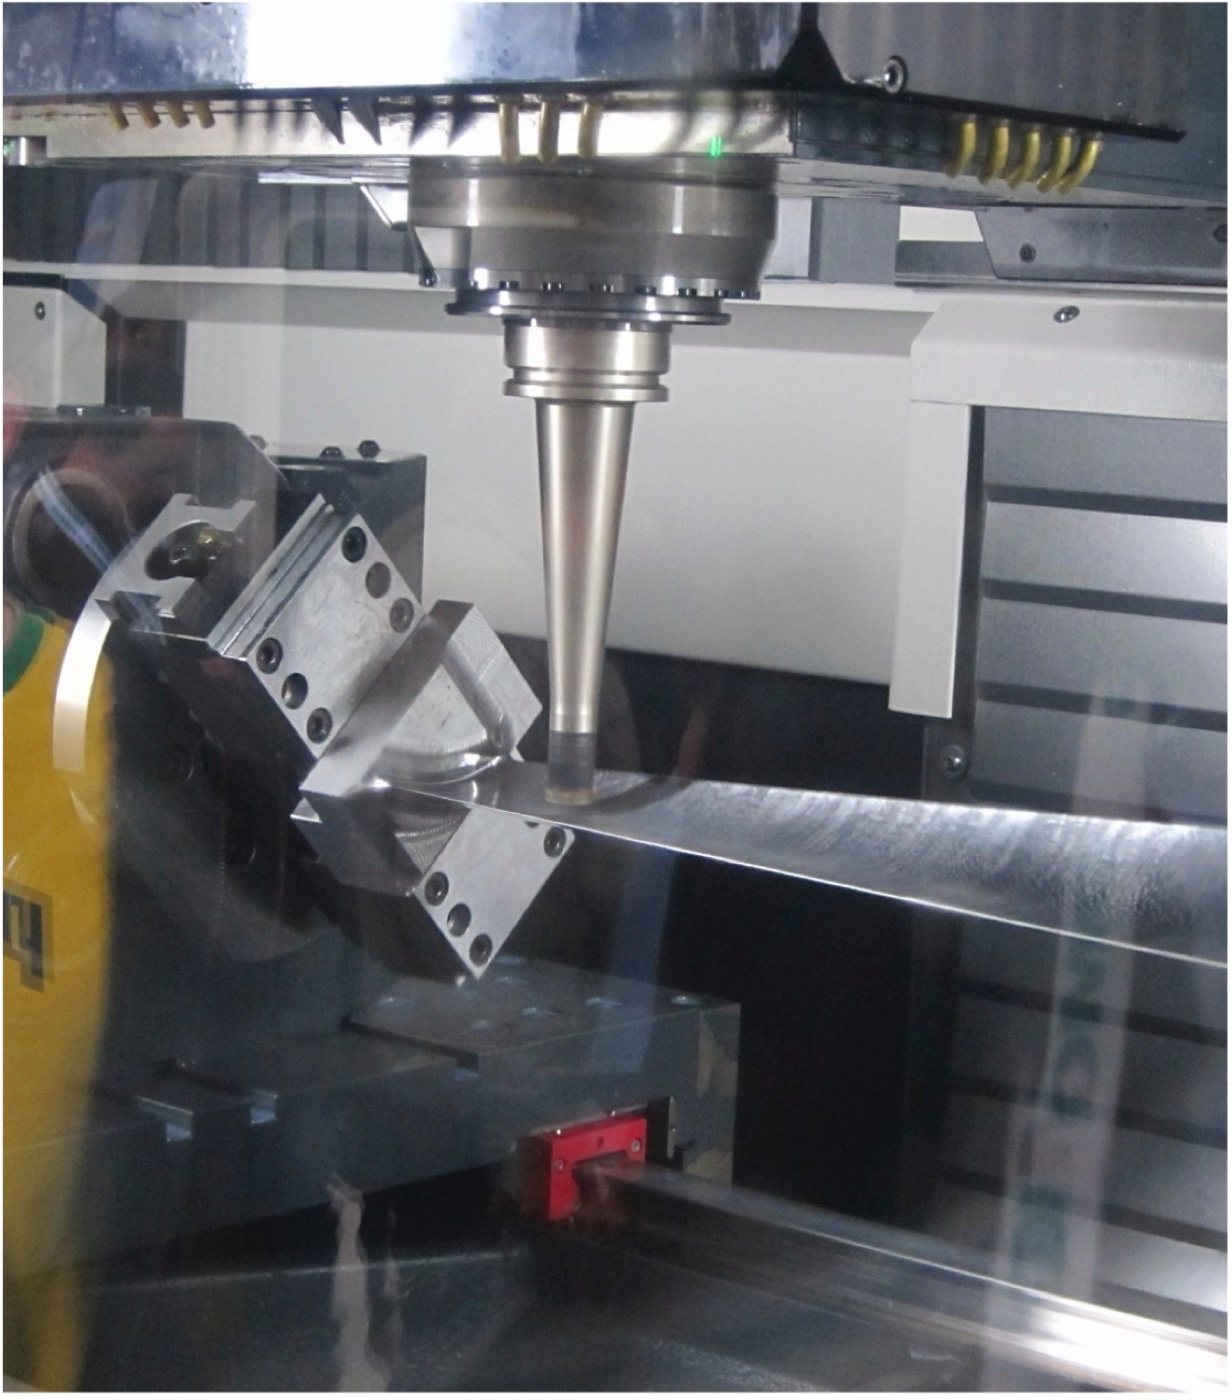
\includegraphics[width=\linewidth,height=4.47917in,keepaspectratio]{images/lathes-photo.jpg}
\end{center}

\subsection{Parallel (engine) lathe}\label{parallel-engine-lathe}

\begin{center}
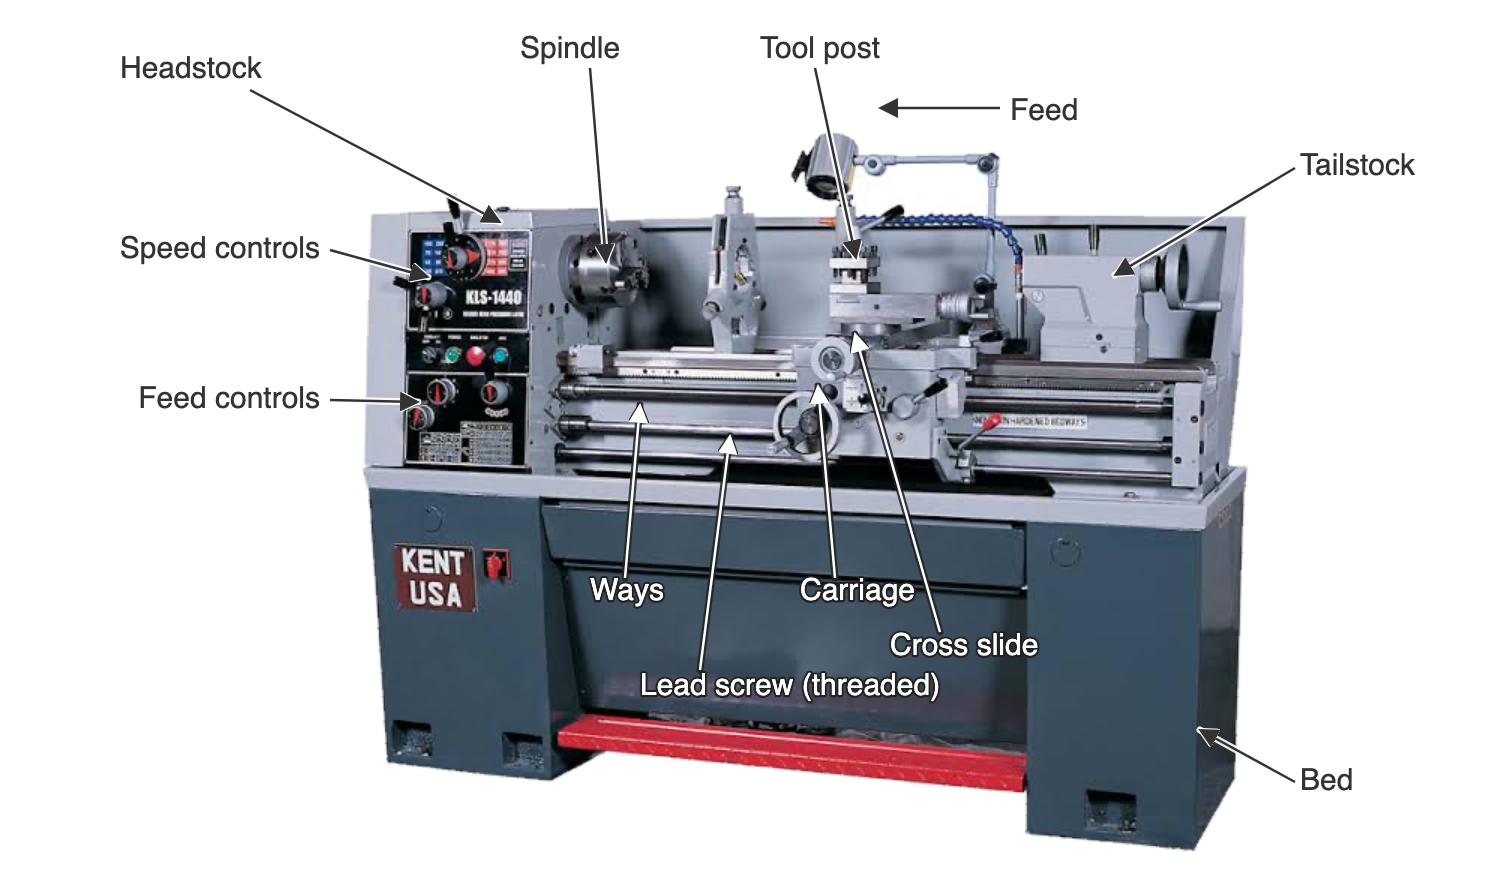
\includegraphics[width=\linewidth,height=4.89583in,keepaspectratio]{images-1/engine-lathe-labeled.png}
\end{center}

\subsection{Parallel (engine) lathe}\label{parallel-engine-lathe-1}

\begin{itemize}
\tightlist
\item
  Programmable engine lathe
\item
  Same architecture as an engine lathe
\item
  Simple controller for programming simple motions (cylinder, cone,
  sphere, plane)
\end{itemize}

\begin{center}
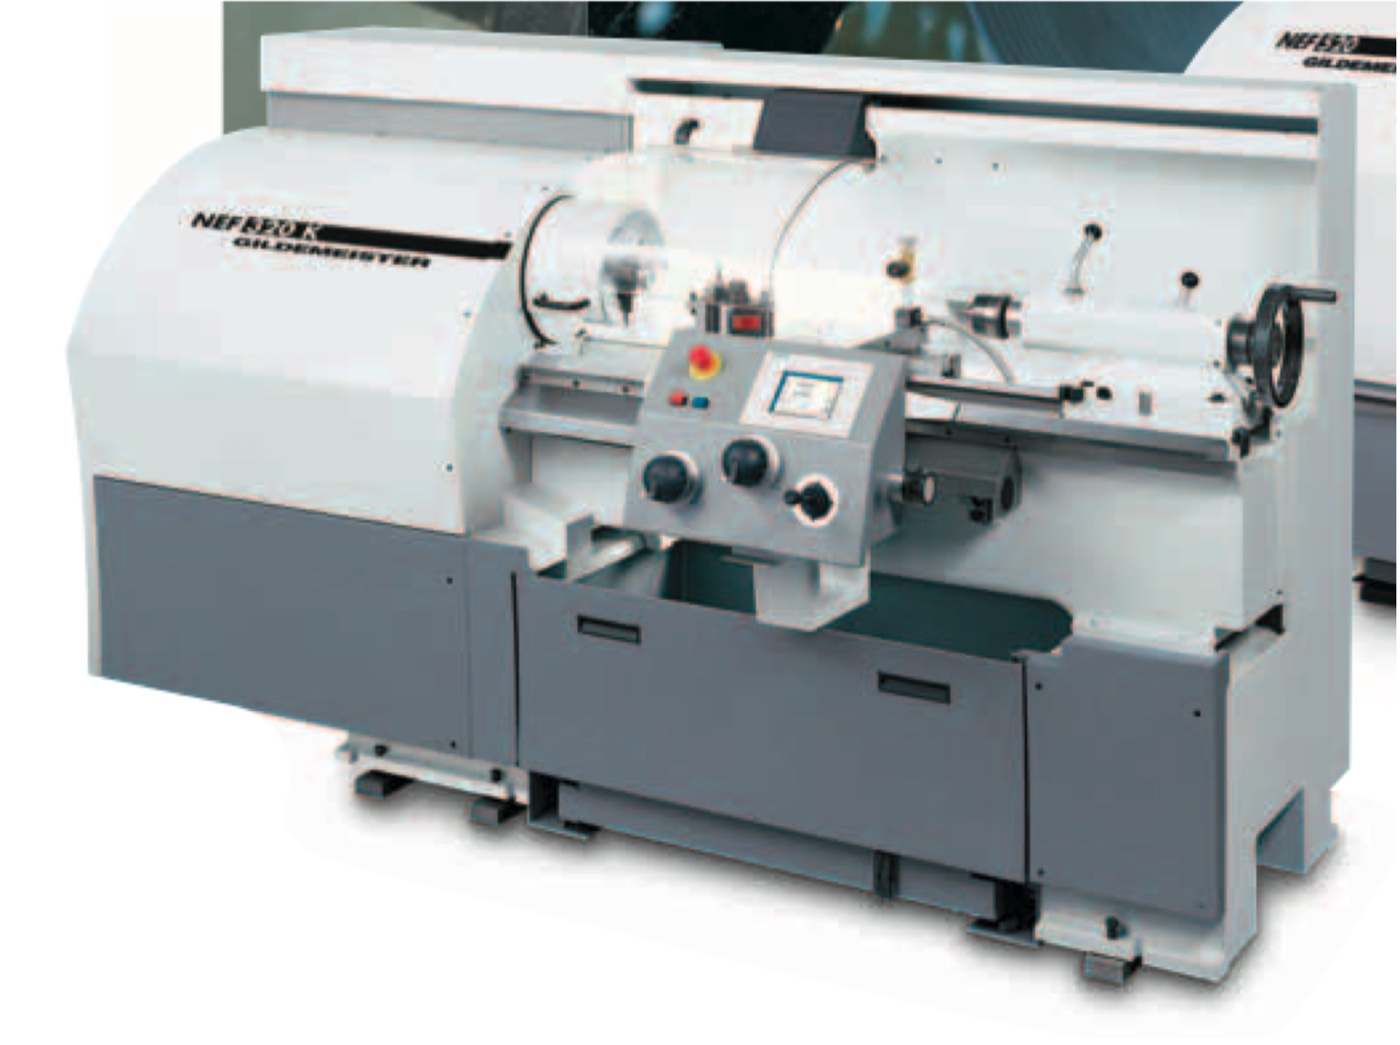
\includegraphics[width=\linewidth,height=3.64583in,keepaspectratio]{images/programmable-lathe.jpg}
\end{center}

\subsection{CNC lathe}\label{cnc-lathe}

\begin{itemize}
\tightlist
\item
  A lathe with enhanced motion controller
  (\textbf{Computer-Numerical-Controller}, CNC)
\item
  Mechanical layout is arranged in order to allow automated chip
  evacuation
\item
  3 controlled axes + spindle, or more
\item
  The spindle can be a controlled axis itself
\item
  It can have rotary tools, too (hybrid turning-milling)
\end{itemize}

\subsection{CNC lathe}\label{cnc-lathe-1}

\begin{itemize}
\tightlist
\item
  Direct-drive spindle
\item
  Roller-turner (revolving) turret
\item
  Counterstock (hydraulics)
\item
  Inclined bed
\item
  Lead screw
\end{itemize}

\begin{center}
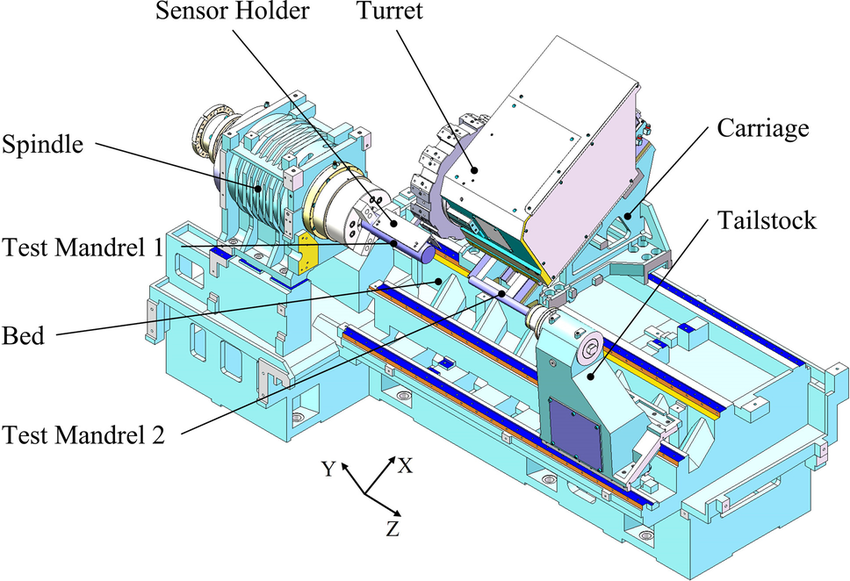
\includegraphics[width=\linewidth,height=4.47917in,keepaspectratio]{images-1/cnc-lathe.png}
\end{center}

\subsection{Moveable rest}\label{moveable-rest}

\begin{center}
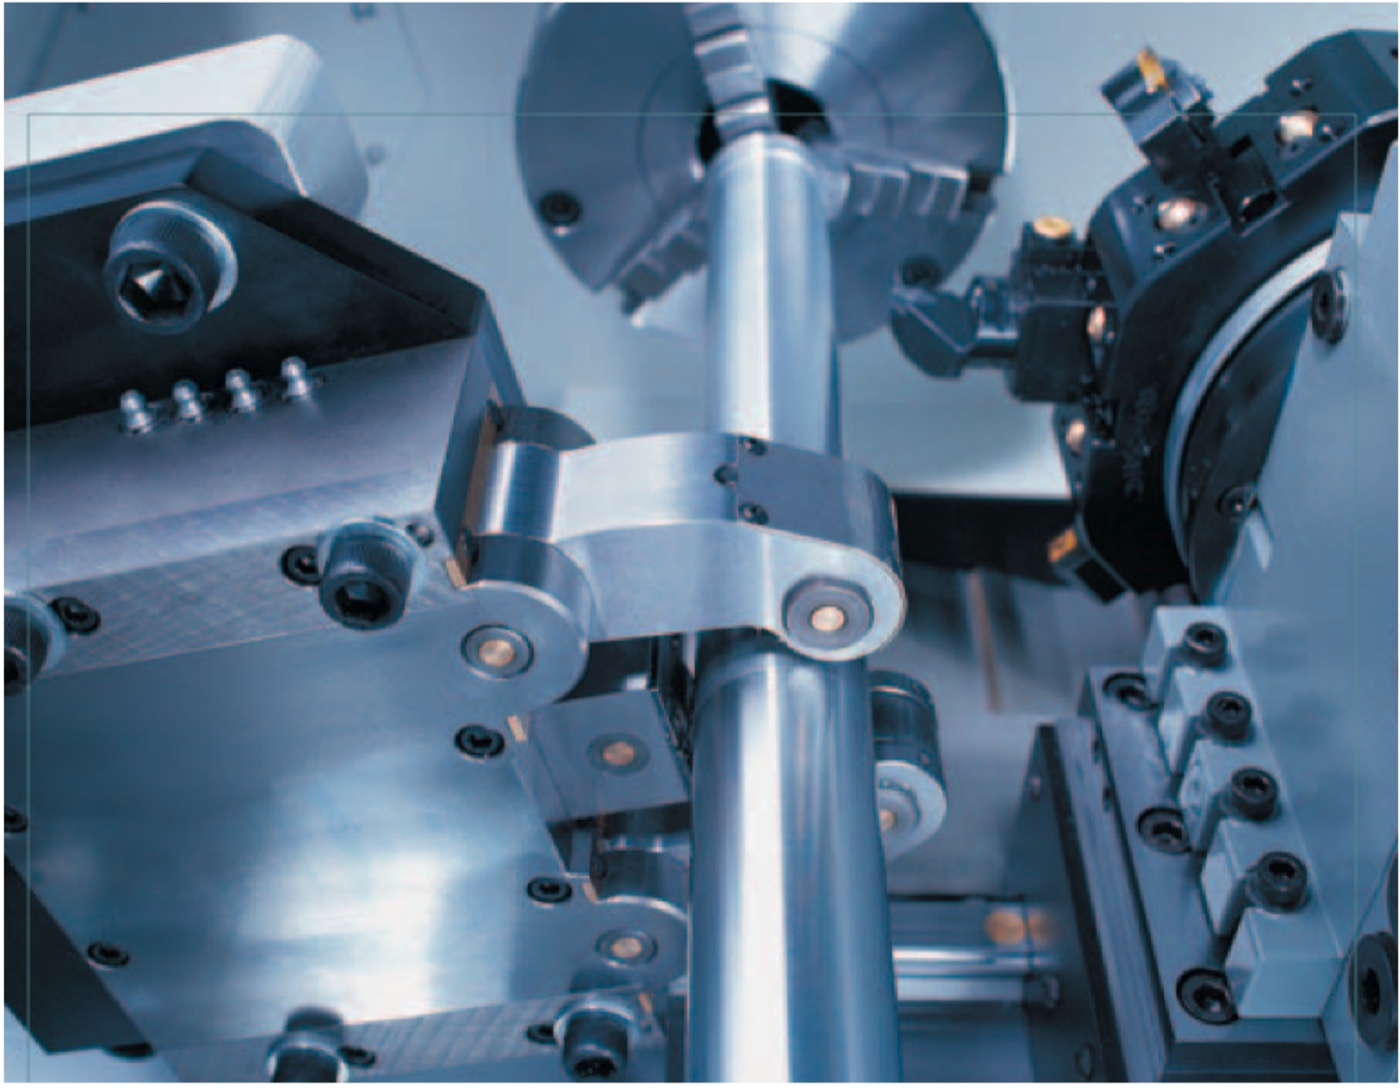
\includegraphics[width=\linewidth,height=4.89583in,keepaspectratio]{images-1/moveable-rest.jpg}
\end{center}

\subsection{Moveable rest}\label{moveable-rest-1}

\subsection{Two-spindle, two turrets
lathe}\label{two-spindle-two-turrets-lathe}

\begin{center}
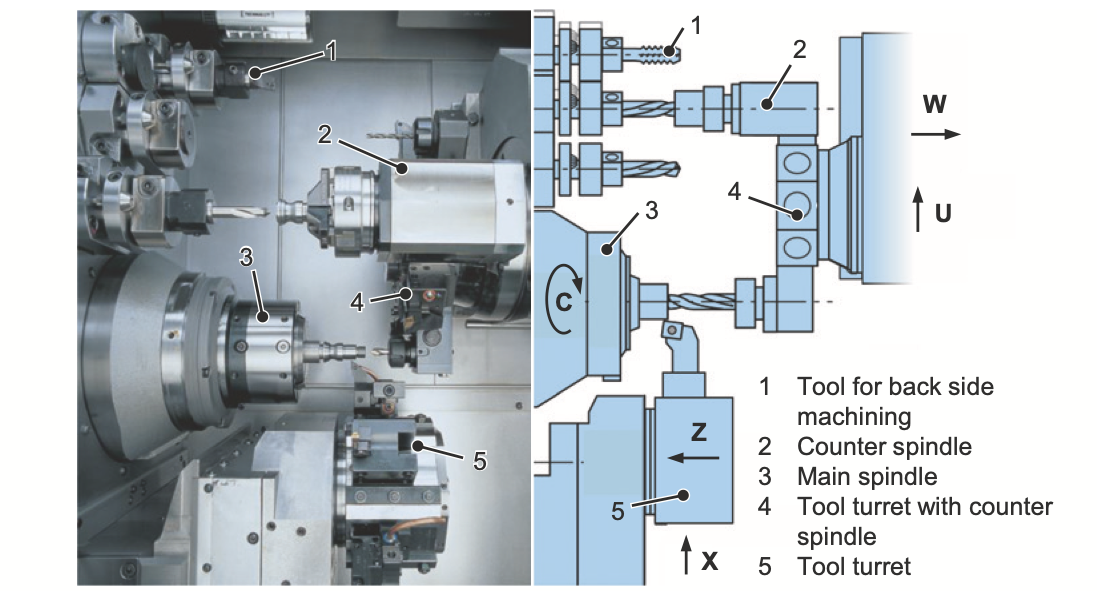
\includegraphics[width=\linewidth,height=4.89583in,keepaspectratio]{images-1/multiple-lathe.png}
\end{center}

\subsection{Multiple spindle lathe}\label{multiple-spindle-lathe}

\begin{center}
\pandocbounded{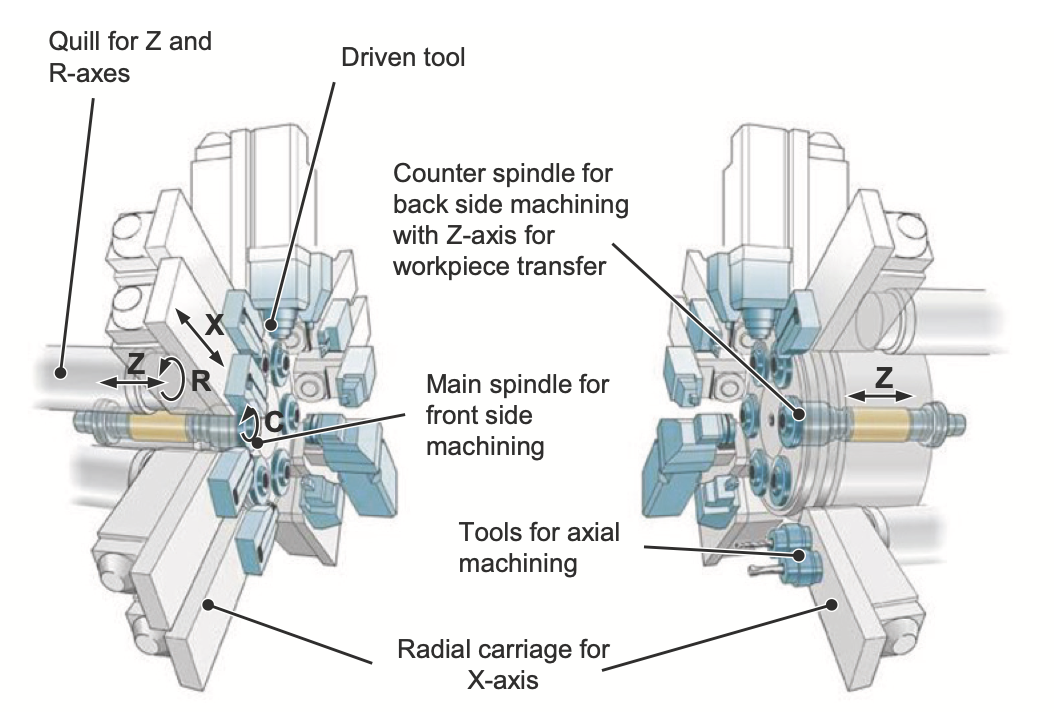
\includegraphics[keepaspectratio]{images-1/multiple-spindle-1.png}}
\end{center}

\subsection{Multiple spindle lathe}\label{multiple-spindle-lathe-1}

\begin{center}
\pandocbounded{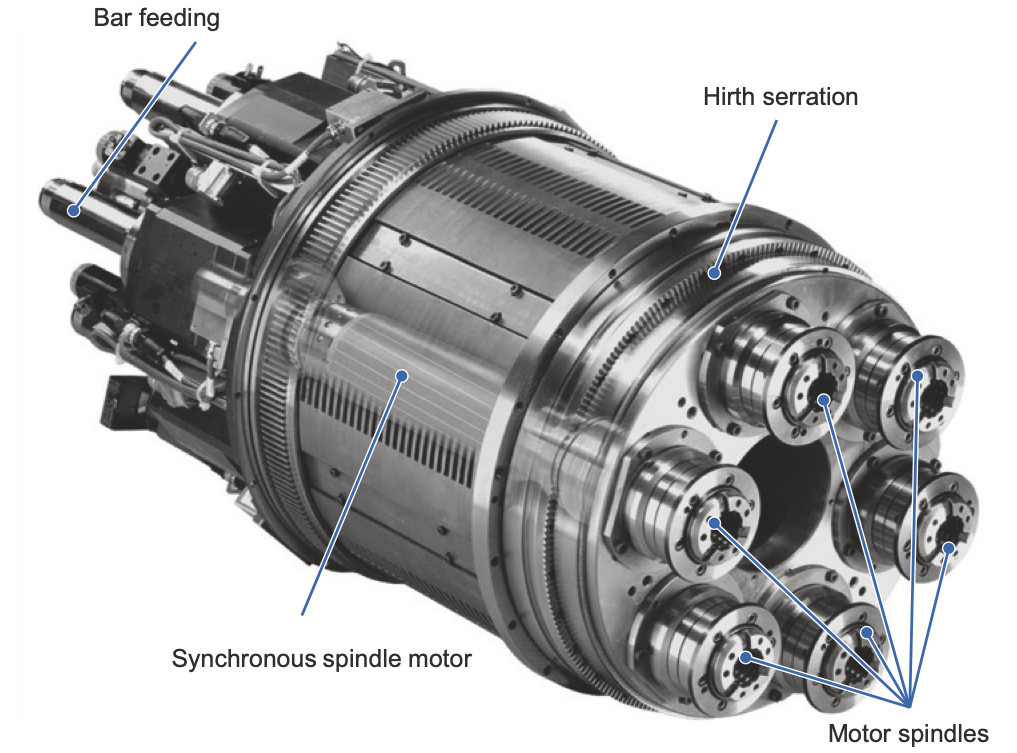
\includegraphics[keepaspectratio]{images-1/multiple-spindle-2.png}}
\end{center}

\subsection{Multiple spindle lathe}\label{multiple-spindle-lathe-2}

\subsection{Vertical spindle lathe}\label{vertical-spindle-lathe}

\begin{figure}[H]

{\centering 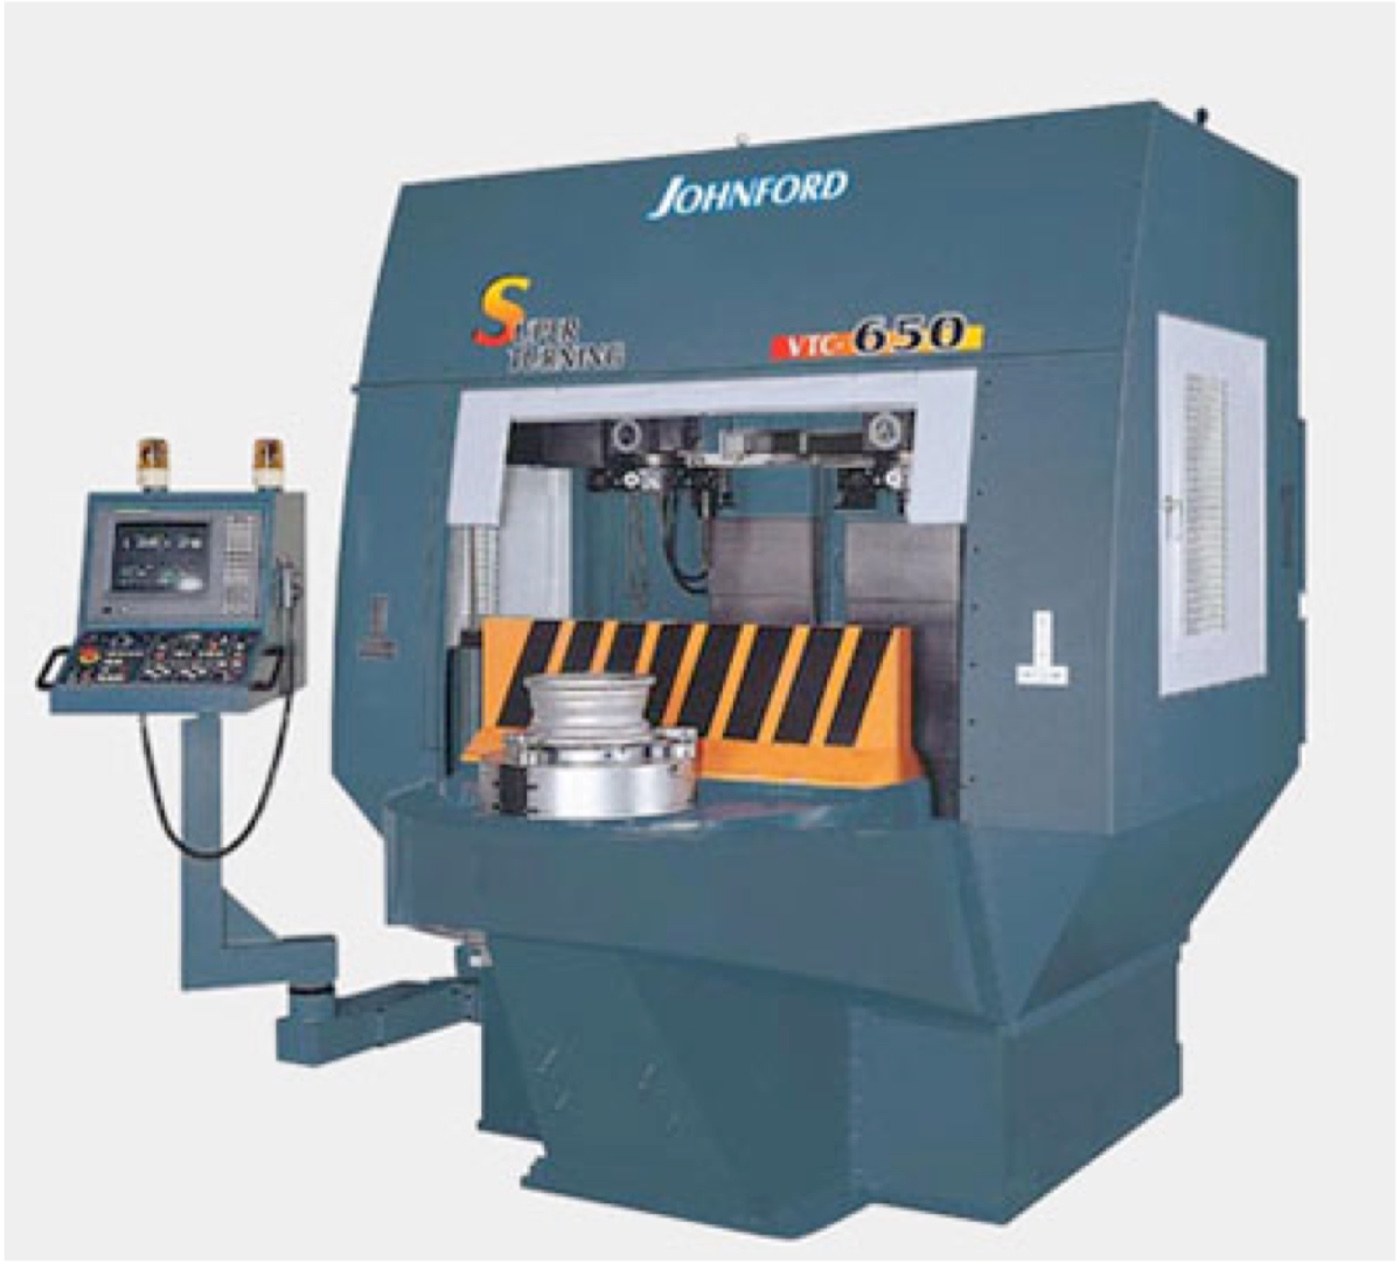
\includegraphics[width=\linewidth,height=5in,keepaspectratio]{images/vertical-normal.jpg}

}

\caption{Normal}

\end{figure}%

\begin{figure}[H]

{\centering 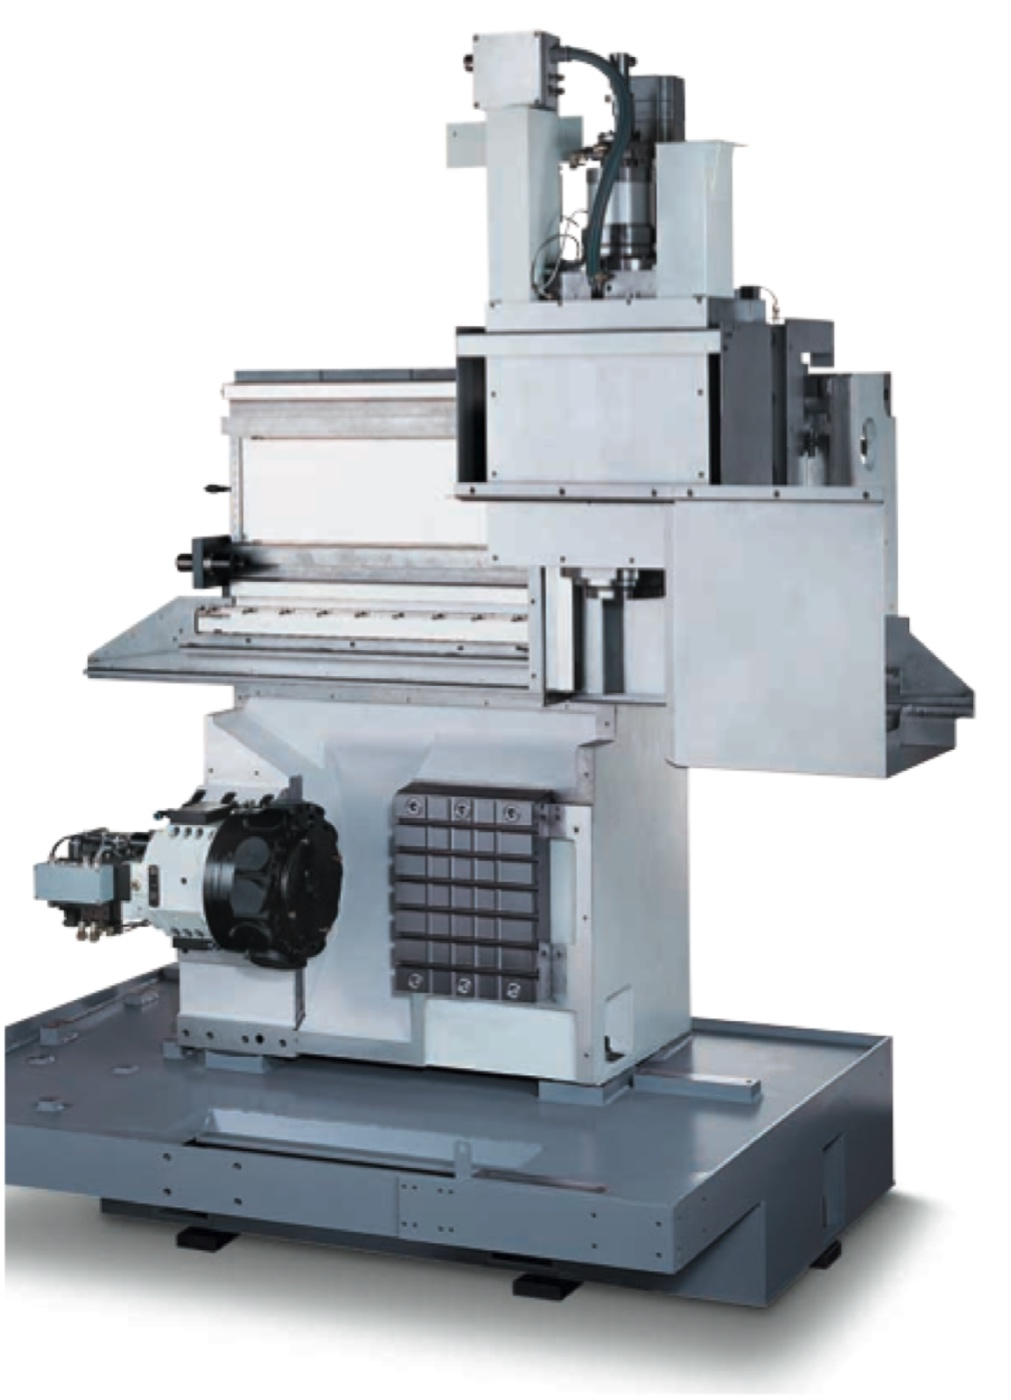
\includegraphics[width=\linewidth,height=5in,keepaspectratio]{images/vertical-inverted.jpg}

}

\caption{Inverted spindle}

\end{figure}%

\subsection{Vertical spindle lathe}\label{vertical-spindle-lathe-1}

\subsection{Sliding headstock}\label{sliding-headstock}

\begin{center}
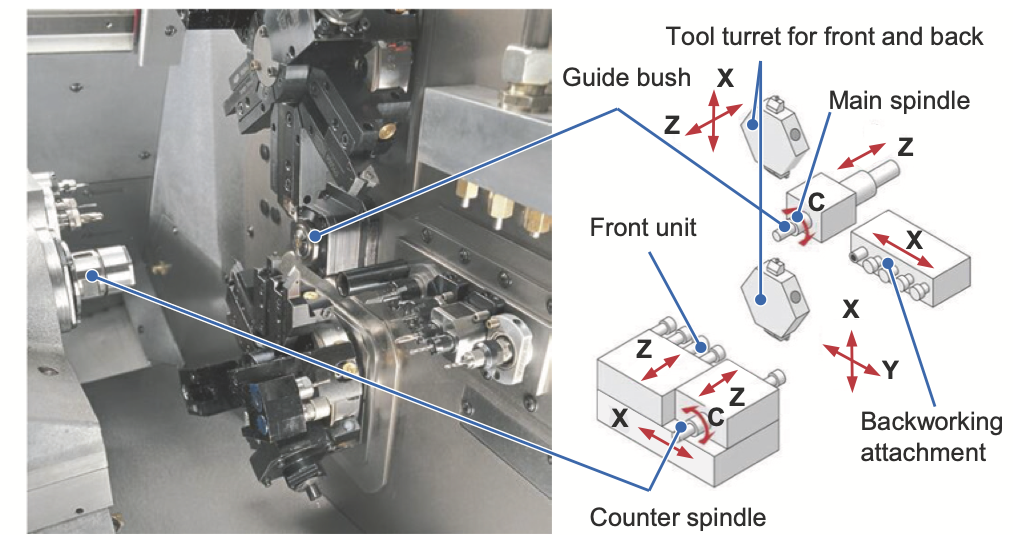
\includegraphics[width=\linewidth,height=5in,keepaspectratio]{images-1/sliding-headstock.png}
\end{center}

\subsection{Sliding headstock}\label{sliding-headstock-1}

\subsection{Parameters}\label{parameters}

\begin{itemize}
\tightlist
\item
  Slewing (\emph{Brandeggio})
\item
  Turning diameter
\item
  Turning length
\item
  X and Z travels (and possibly other axes)
\item
  Spindle speed
\item
  Rapid speeds
\item
  Spindle torque and power
\end{itemize}

\begin{figure}[H]

{\centering 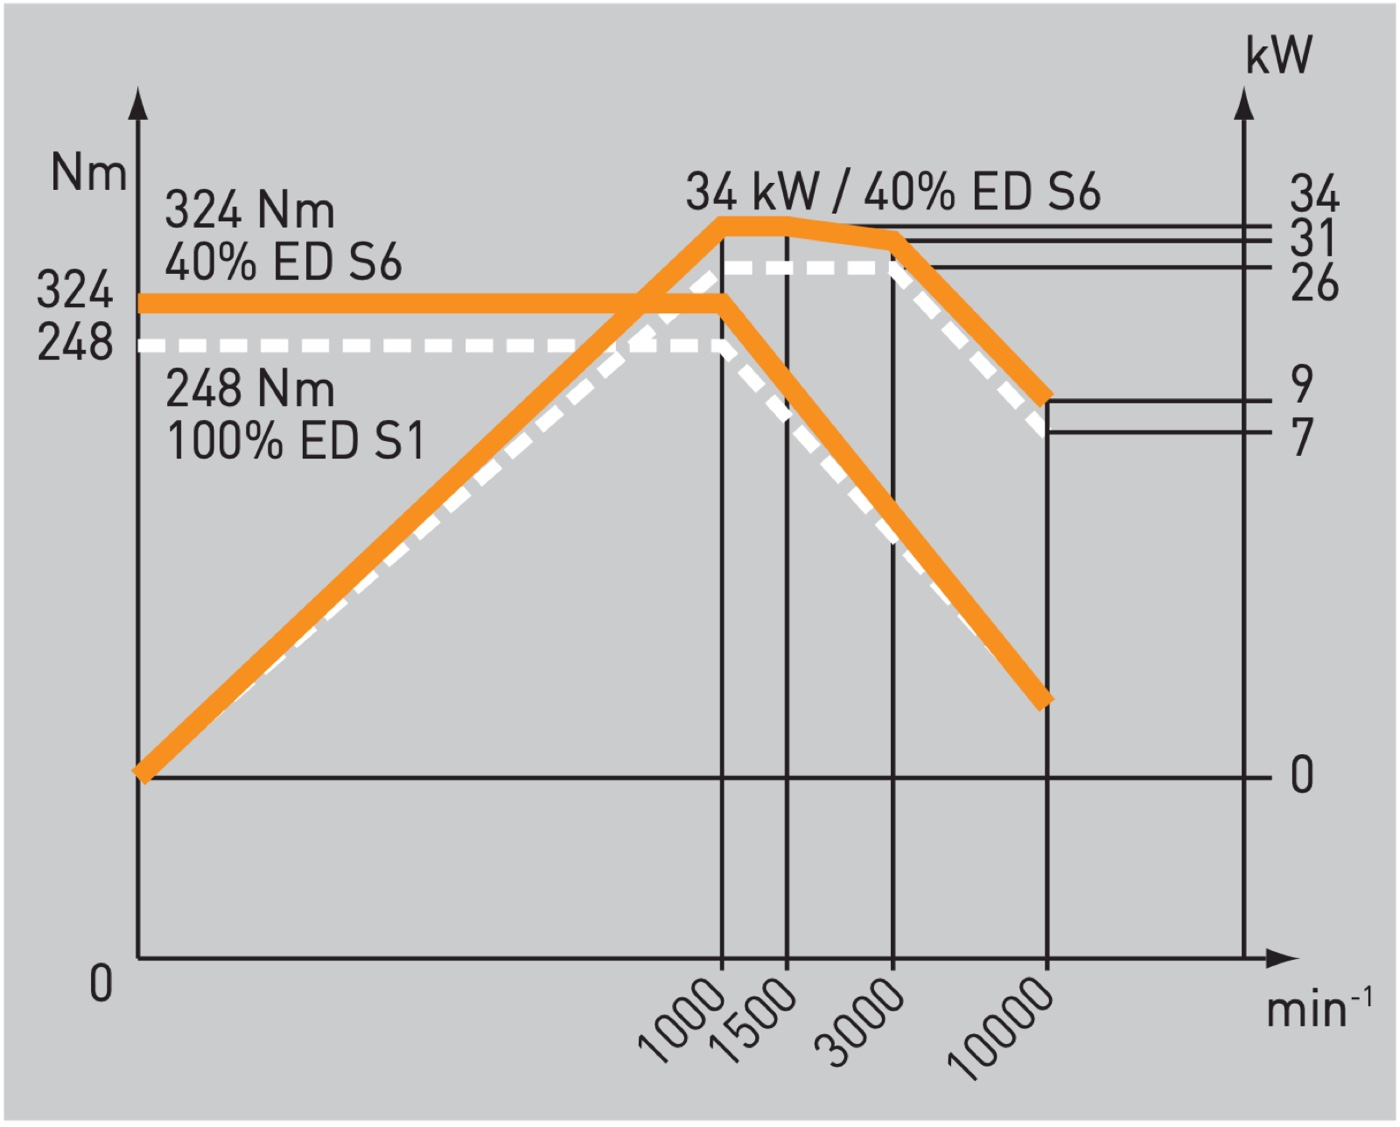
\includegraphics[width=0.8\linewidth,height=\textheight,keepaspectratio]{images/spindle-power.jpg}

}

\caption{ED = \emph{Einschaltdauer} (operating time)}

\end{figure}%

ED= Duty Cycle=moving time / total cycle time. S6 = ED 40\%

\subsection{Milling machines}\label{milling-machines}

\begin{itemize}
\tightlist
\item
  Huge variety of architectures
\item
  Common denominator: rotary tool
\item
  From desktop size to 200 m\(^3\) footprint
\item
  Some have rotary table and can do turning (hybrid mill-turn)
\end{itemize}

\begin{center}
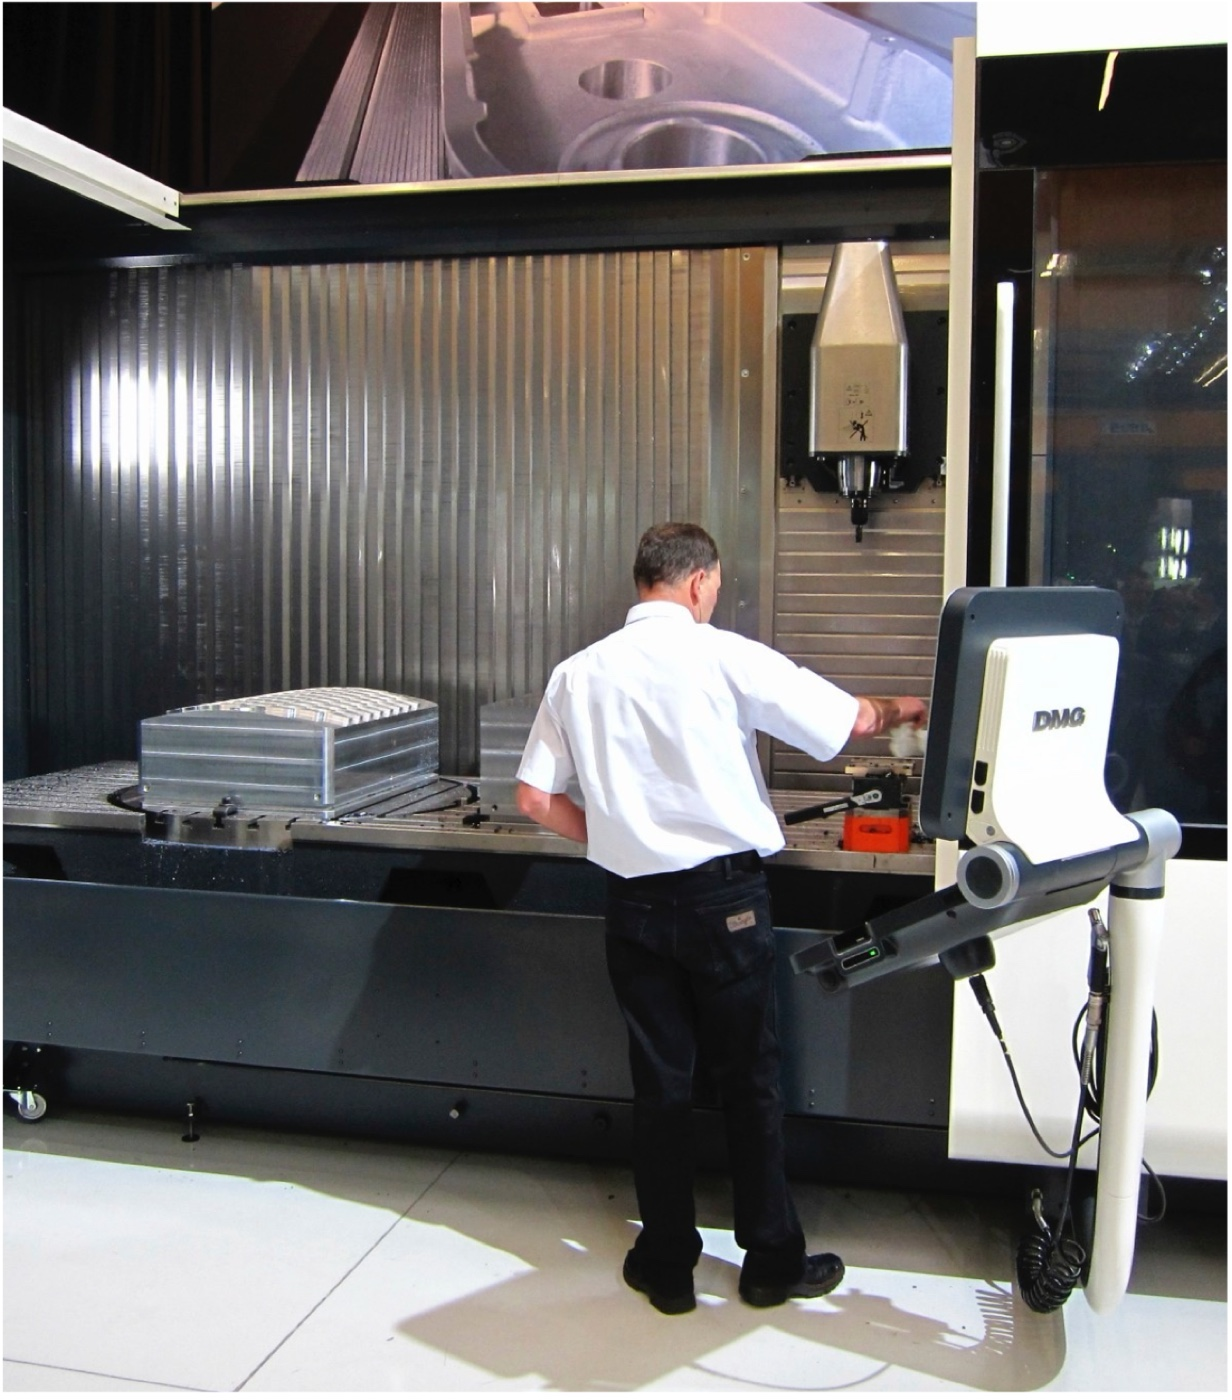
\includegraphics[width=\linewidth,height=4.16667in,keepaspectratio]{images/milling-machine.jpg}
\end{center}

\subsection{Types of Milling Machines}\label{types-of-milling-machines}

\begin{itemize}
\tightlist
\item
  CNC Milling Machines

  \begin{itemize}
  \tightlist
  \item
    Horizontal spindle
  \item
    Vertical spindle
  \end{itemize}
\item
  Milling centers

  \begin{itemize}
  \tightlist
  \item
    Universal
  \item
    Pallet changer
  \item
    Traveling column
  \end{itemize}
\item
  Architectures

  \begin{itemize}
  \tightlist
  \item
    Cantilever
  \item
    Traveling column
  \item
    Gantry
  \item
    Parallel kinematics
  \end{itemize}
\end{itemize}

\begin{figure}[H]

{\centering 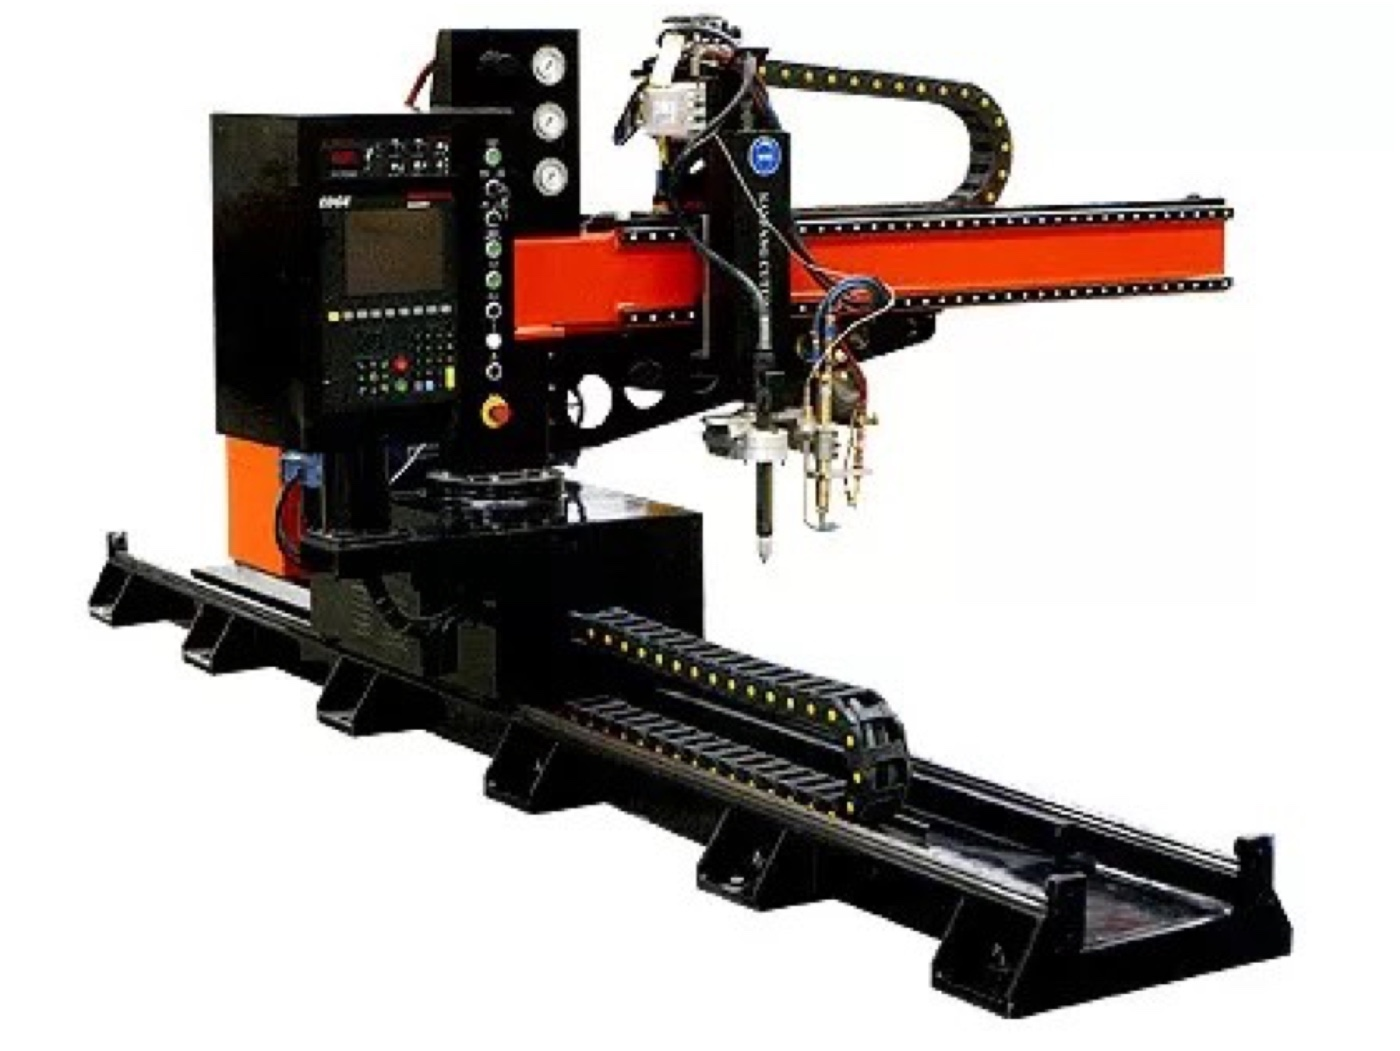
\includegraphics[width=\linewidth,height=2.5in,keepaspectratio]{images-1/cantilever.jpg}

}

\caption{Cantilever}

\end{figure}%

\begin{figure}[H]

{\centering 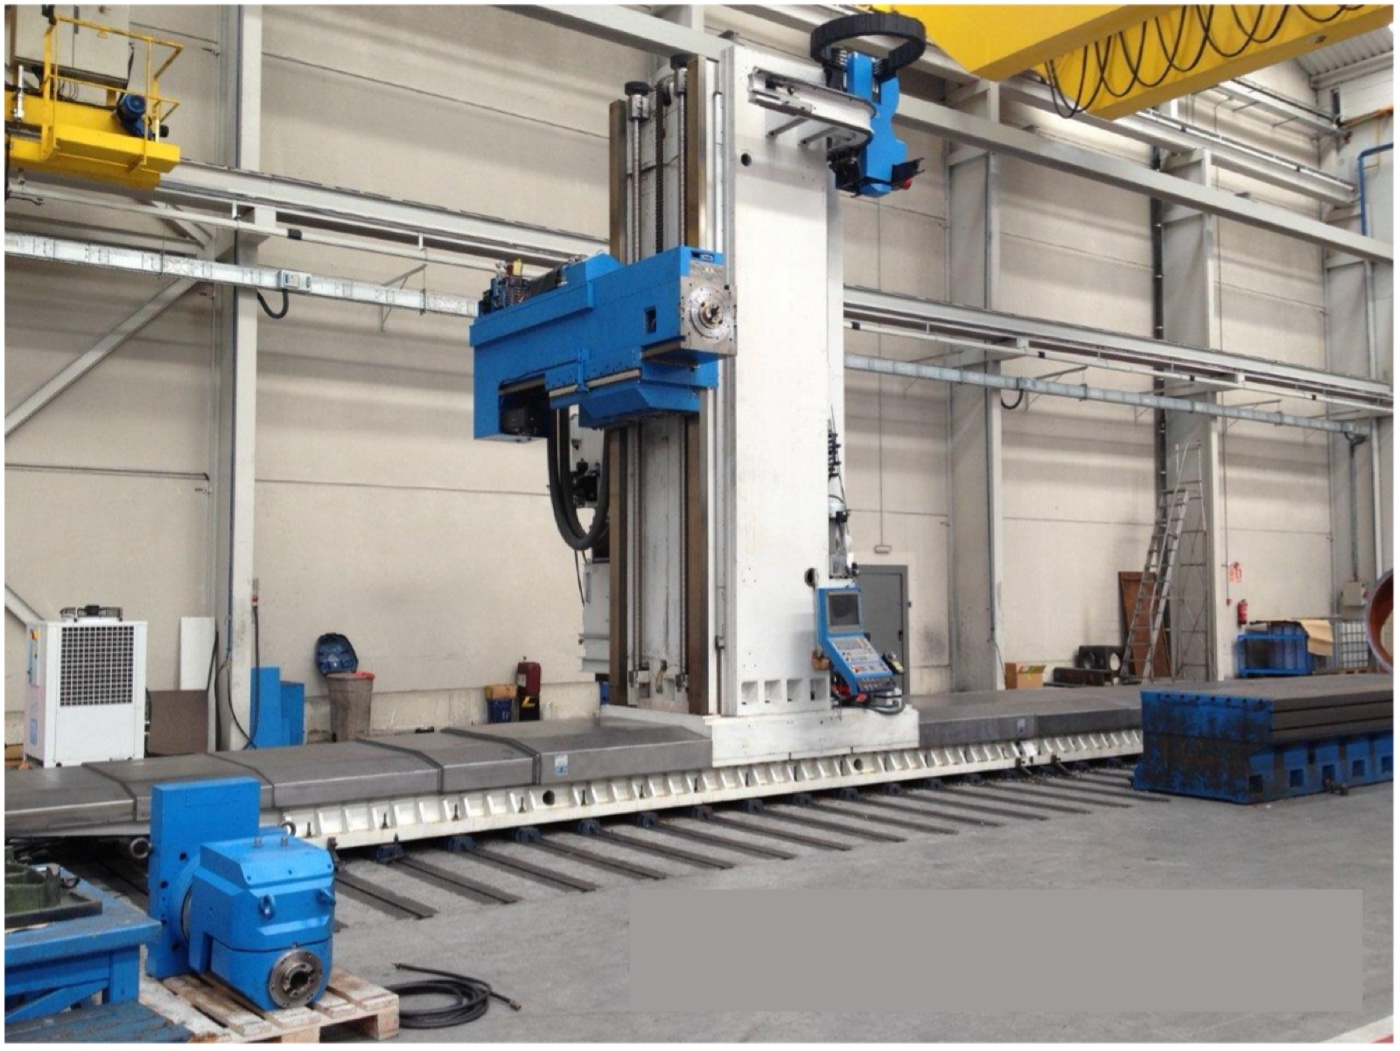
\includegraphics[width=\linewidth,height=2.5in,keepaspectratio]{images-1/travelling-column.jpg}

}

\caption{Travelling column}

\end{figure}%

\begin{figure}[H]

{\centering 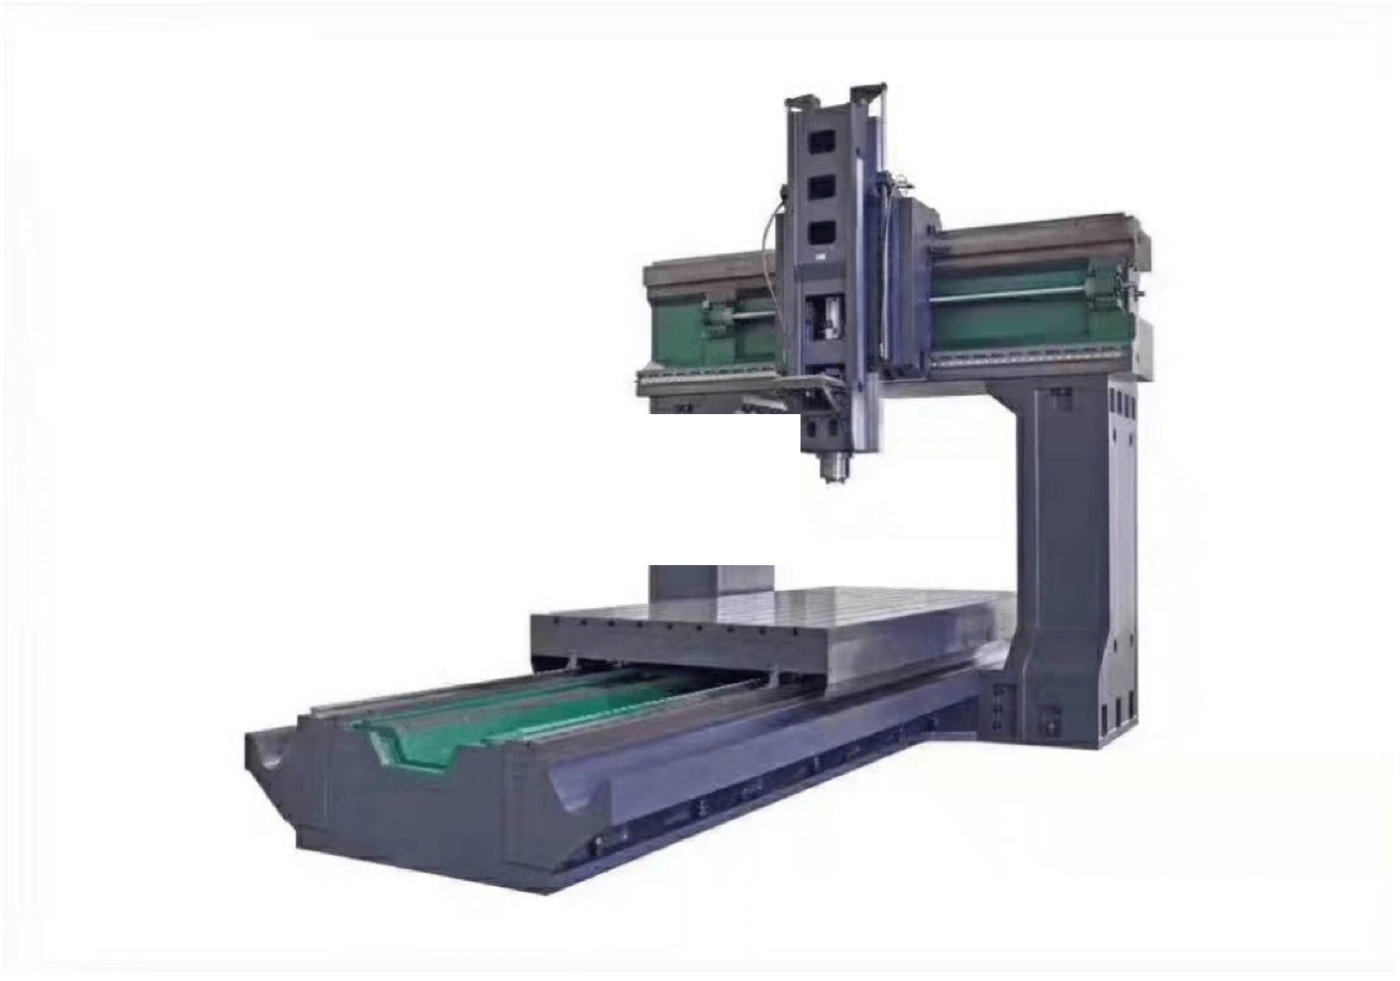
\includegraphics[width=\linewidth,height=2.5in,keepaspectratio]{images-1/gantry.jpg}

}

\caption{Gantry}

\end{figure}%

\begin{figure}[H]

{\centering 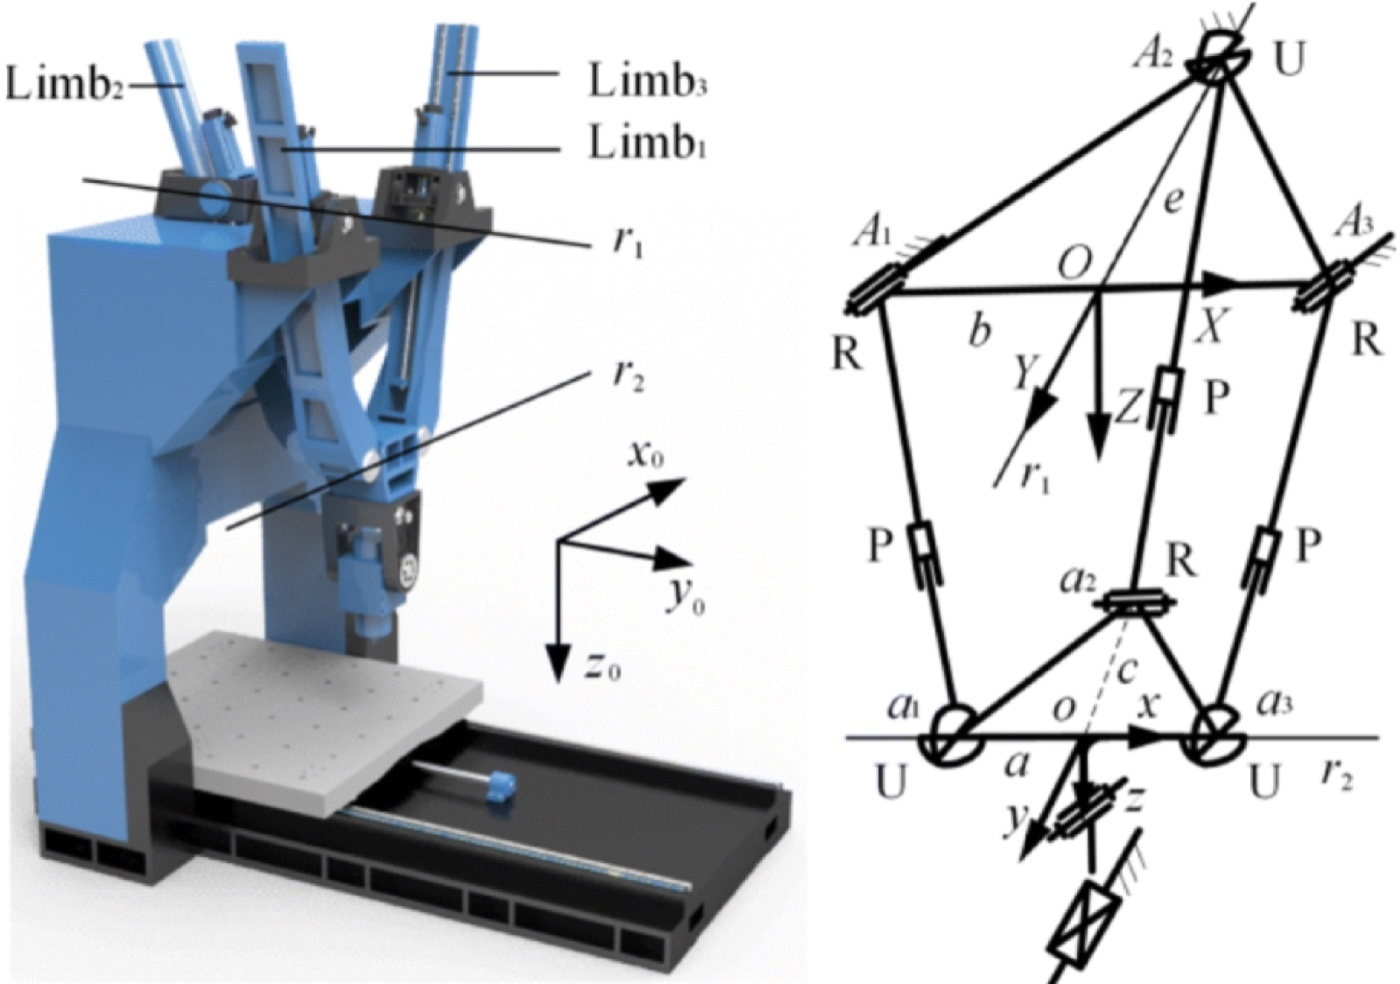
\includegraphics[width=\linewidth,height=2.5in,keepaspectratio]{images-1/parallel-kinematics.jpg}

}

\caption{Parallel kinematics}

\end{figure}%

\subsection{Universal milling center}\label{universal-milling-center}

\begin{itemize}
\tightlist
\item
  Universal milling centers have a \textbf{rotary table} and a
  \textbf{universal milling head} that can be tilted and swiveled to
  machine any surface of the workpiece
\item
  By rotating the axis at 45° from Z, the spindle axis can be changed
  from vertical to horizontal (\emph{universal})
\end{itemize}

\begin{figure}[H]

{\centering 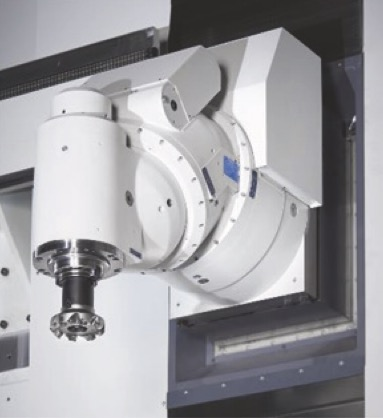
\includegraphics[width=\linewidth,height=4.16667in,keepaspectratio]{images-1/universal-head.jpg}

}

\caption{Universal milling head}

\end{figure}%

\subsection{Architectures}\label{architectures}

\begin{itemize}
\tightlist
\item
  \textbf{Cantilever:} simplest and cheapest
\item
  \textbf{Traveling column:} suitable when one axis is much longer
\item
  \textbf{Gantry:} much more stiff and stable, but more complex (twin
  axes)
\item
  \textbf{Parallel-K:} much stiffer and faster, but complex to control
  and limited in travels
\end{itemize}

\begin{center}
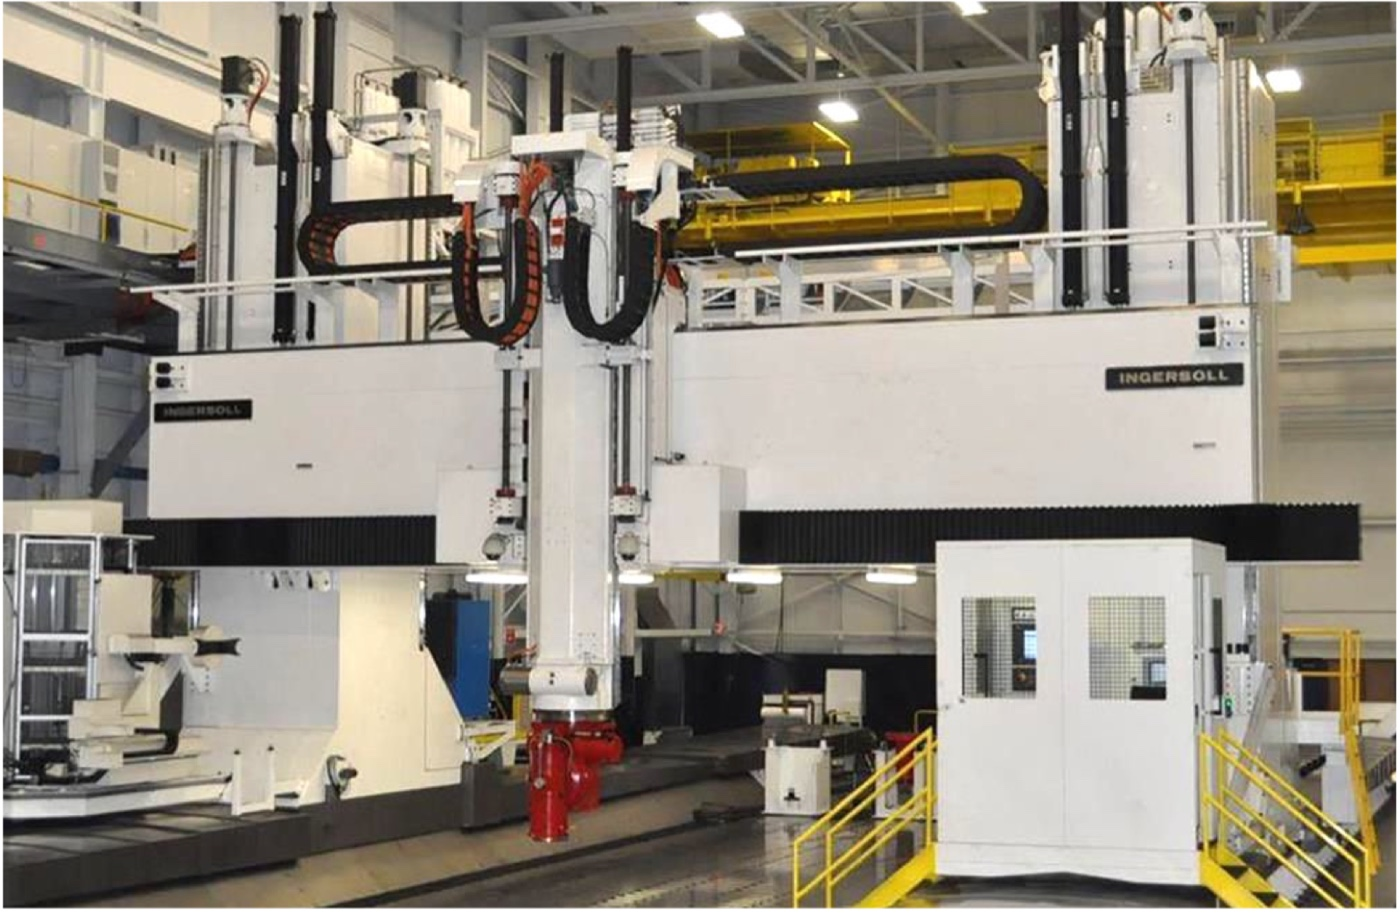
\includegraphics[width=\linewidth,height=3.4375in,keepaspectratio]{images/architectures.jpg}
\end{center}

\subsection{Vertical spindle}\label{vertical-spindle}

{Pros}:

\begin{itemize}
\tightlist
\item
  Easy fixturing
\item
  Reduced moveable mass
\end{itemize}

\textbf{Cons}:

\begin{itemize}
\tightlist
\item
  Chip disposal is more difficult
\item
  Not suitable for machining dies/cavities
\end{itemize}

\begin{figure}[H]

{\centering \pandocbounded{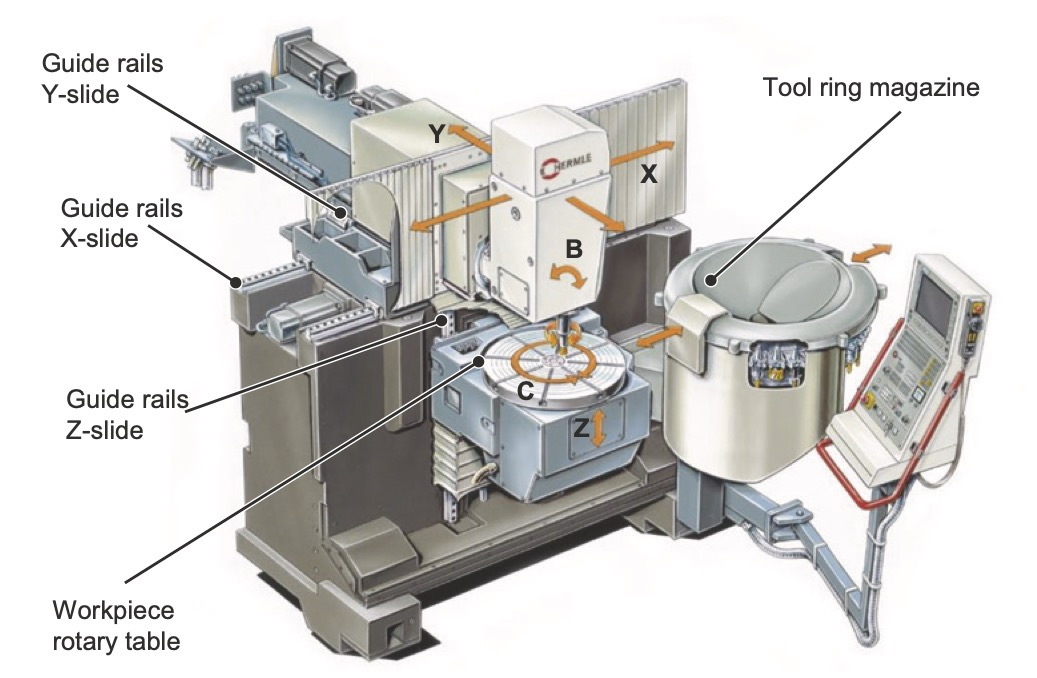
\includegraphics[keepaspectratio]{images-1/vertical-spindle.jpg}}

}

\caption{Vertical spindle machine}

\end{figure}%

\subsection{Horizontal spindle}\label{horizontal-spindle}

{Pros}:

\begin{itemize}
\tightlist
\item
  Better chip/liquids disposal
\item
  Large travels
\end{itemize}

\textbf{Cons}:

\begin{itemize}
\tightlist
\item
  More difficult fixturing
\item
  More moveable mass (slower)
\item
  more difficult to fixture
\end{itemize}

\begin{figure}[H]

{\centering \pandocbounded{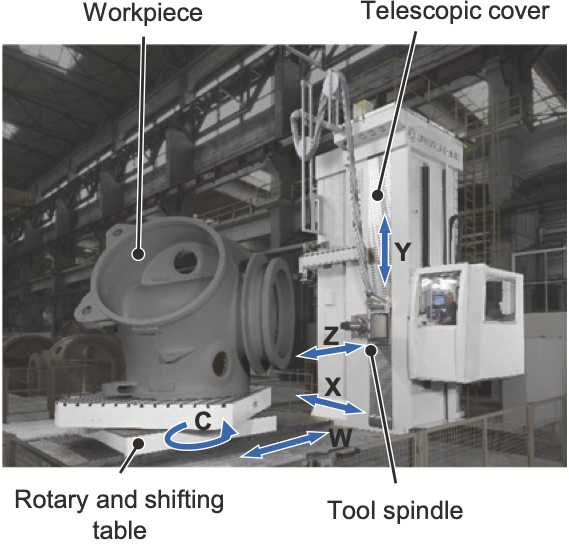
\includegraphics[keepaspectratio]{images-1/horizontal-spindle.png}}

}

\caption{Horizontal spindle machine}

\end{figure}%

\subsection{Pallet changer}\label{pallet-changer}

\begin{itemize}
\tightlist
\item
  Stocky WPs
\item
  High productivity
\item
  can be integrated in automated lines
\end{itemize}

\begin{figure}[H]

{\centering \pandocbounded{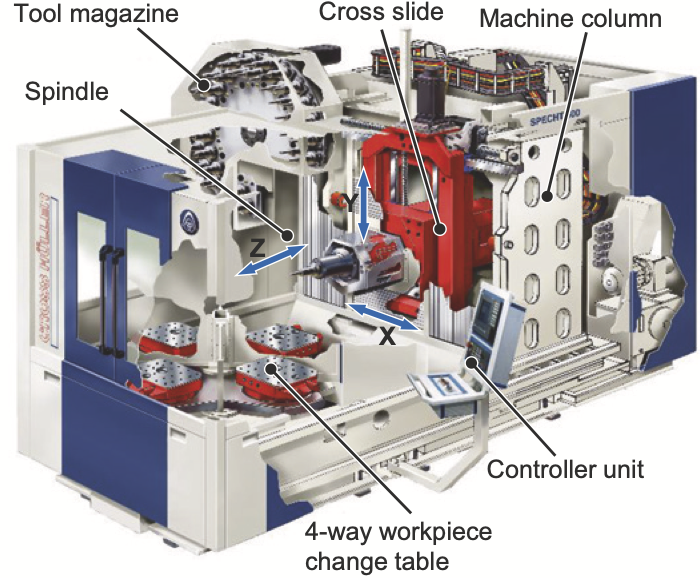
\includegraphics[keepaspectratio]{images-1/pallet-changer-machine.png}}

}

\caption{Pallet changer}

\end{figure}%

\subsection{Traveling column}\label{traveling-column}

Suitable for:

\begin{itemize}
\tightlist
\item
  slender WP
\item
  stocky WP but with two alternating fixturing zones (higher
  productivity)
\end{itemize}

\begin{tcolorbox}[enhanced jigsaw, arc=.35mm, bottomrule=.15mm, bottomtitle=1mm, breakable, colback=white, colbacktitle=quarto-callout-important-color!10!white, colframe=quarto-callout-important-color-frame, coltitle=black, left=2mm, leftrule=.75mm, opacityback=0, opacitybacktitle=0.6, rightrule=.15mm, title=\textcolor{quarto-callout-important-color}{\faExclamation}\hspace{0.5em}{Masked time}, titlerule=0mm, toprule=.15mm, toptitle=1mm]

Any operation that can be performed in parallel to machining is said to
happen in \emph{masked time}. Its cost is absorbed in the machining cost

Other operations happen in \emph{exposed time}, which is added to the
machining cost

\end{tcolorbox}

\begin{figure}[H]

{\centering \pandocbounded{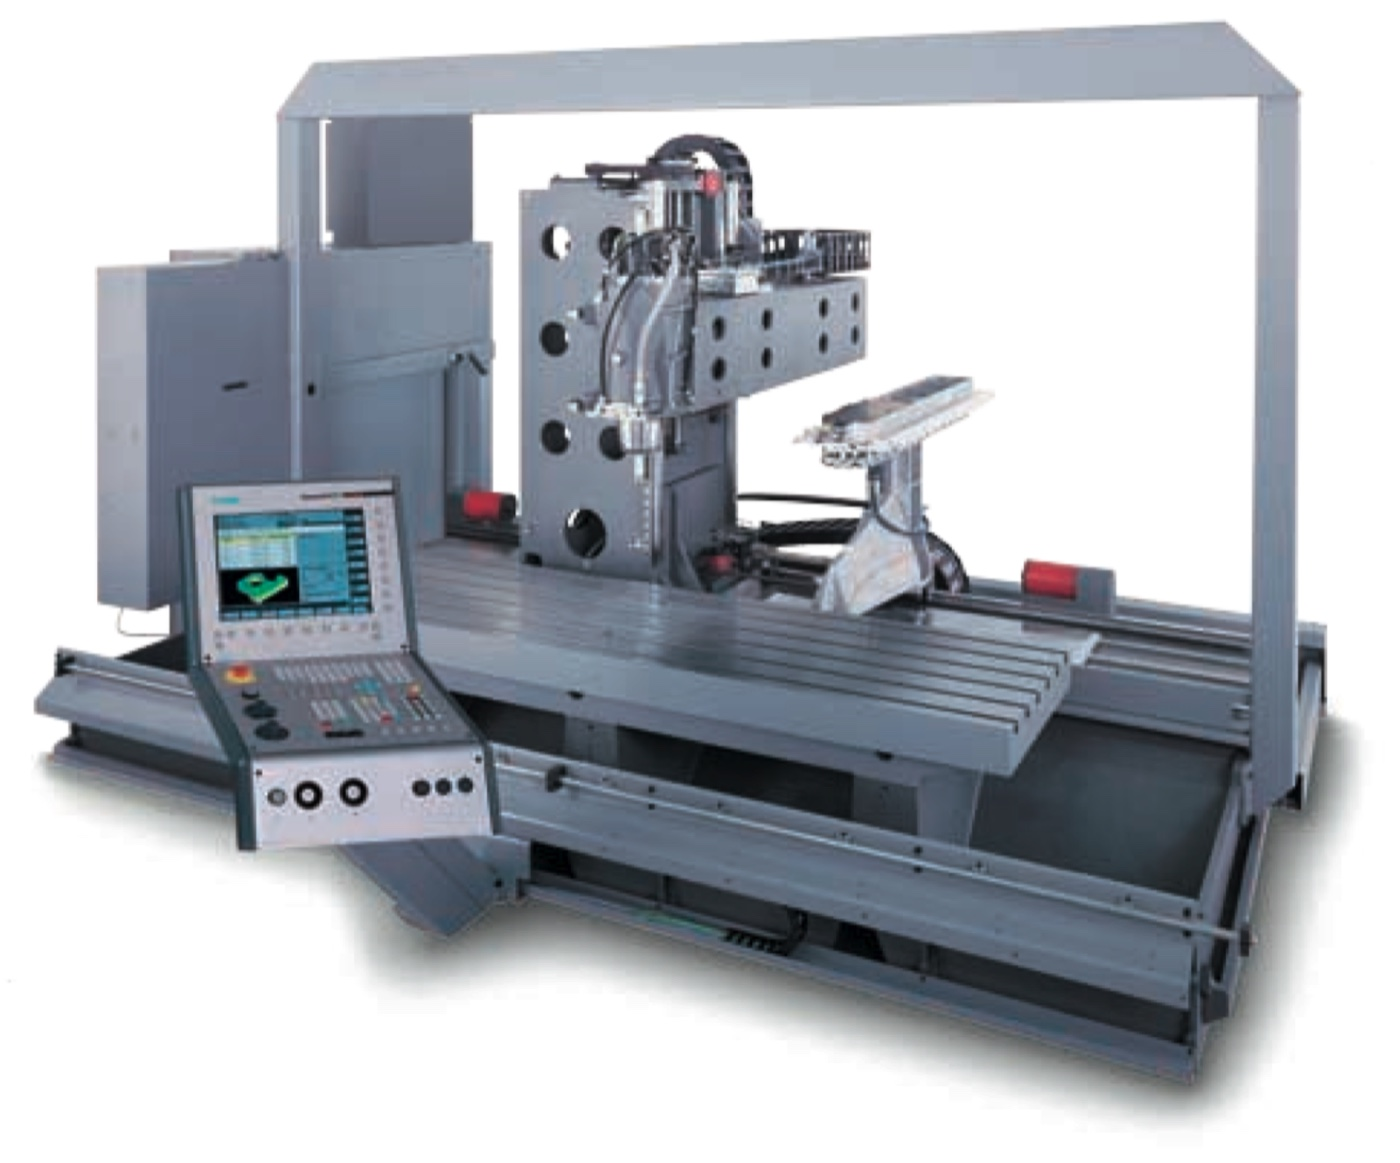
\includegraphics[keepaspectratio]{images-1/traveling-column.jpg}}

}

\caption{Travelling column machine}

\end{figure}%

\subsection{Milling centers}\label{milling-centers}

\begin{figure}[H]

{\centering 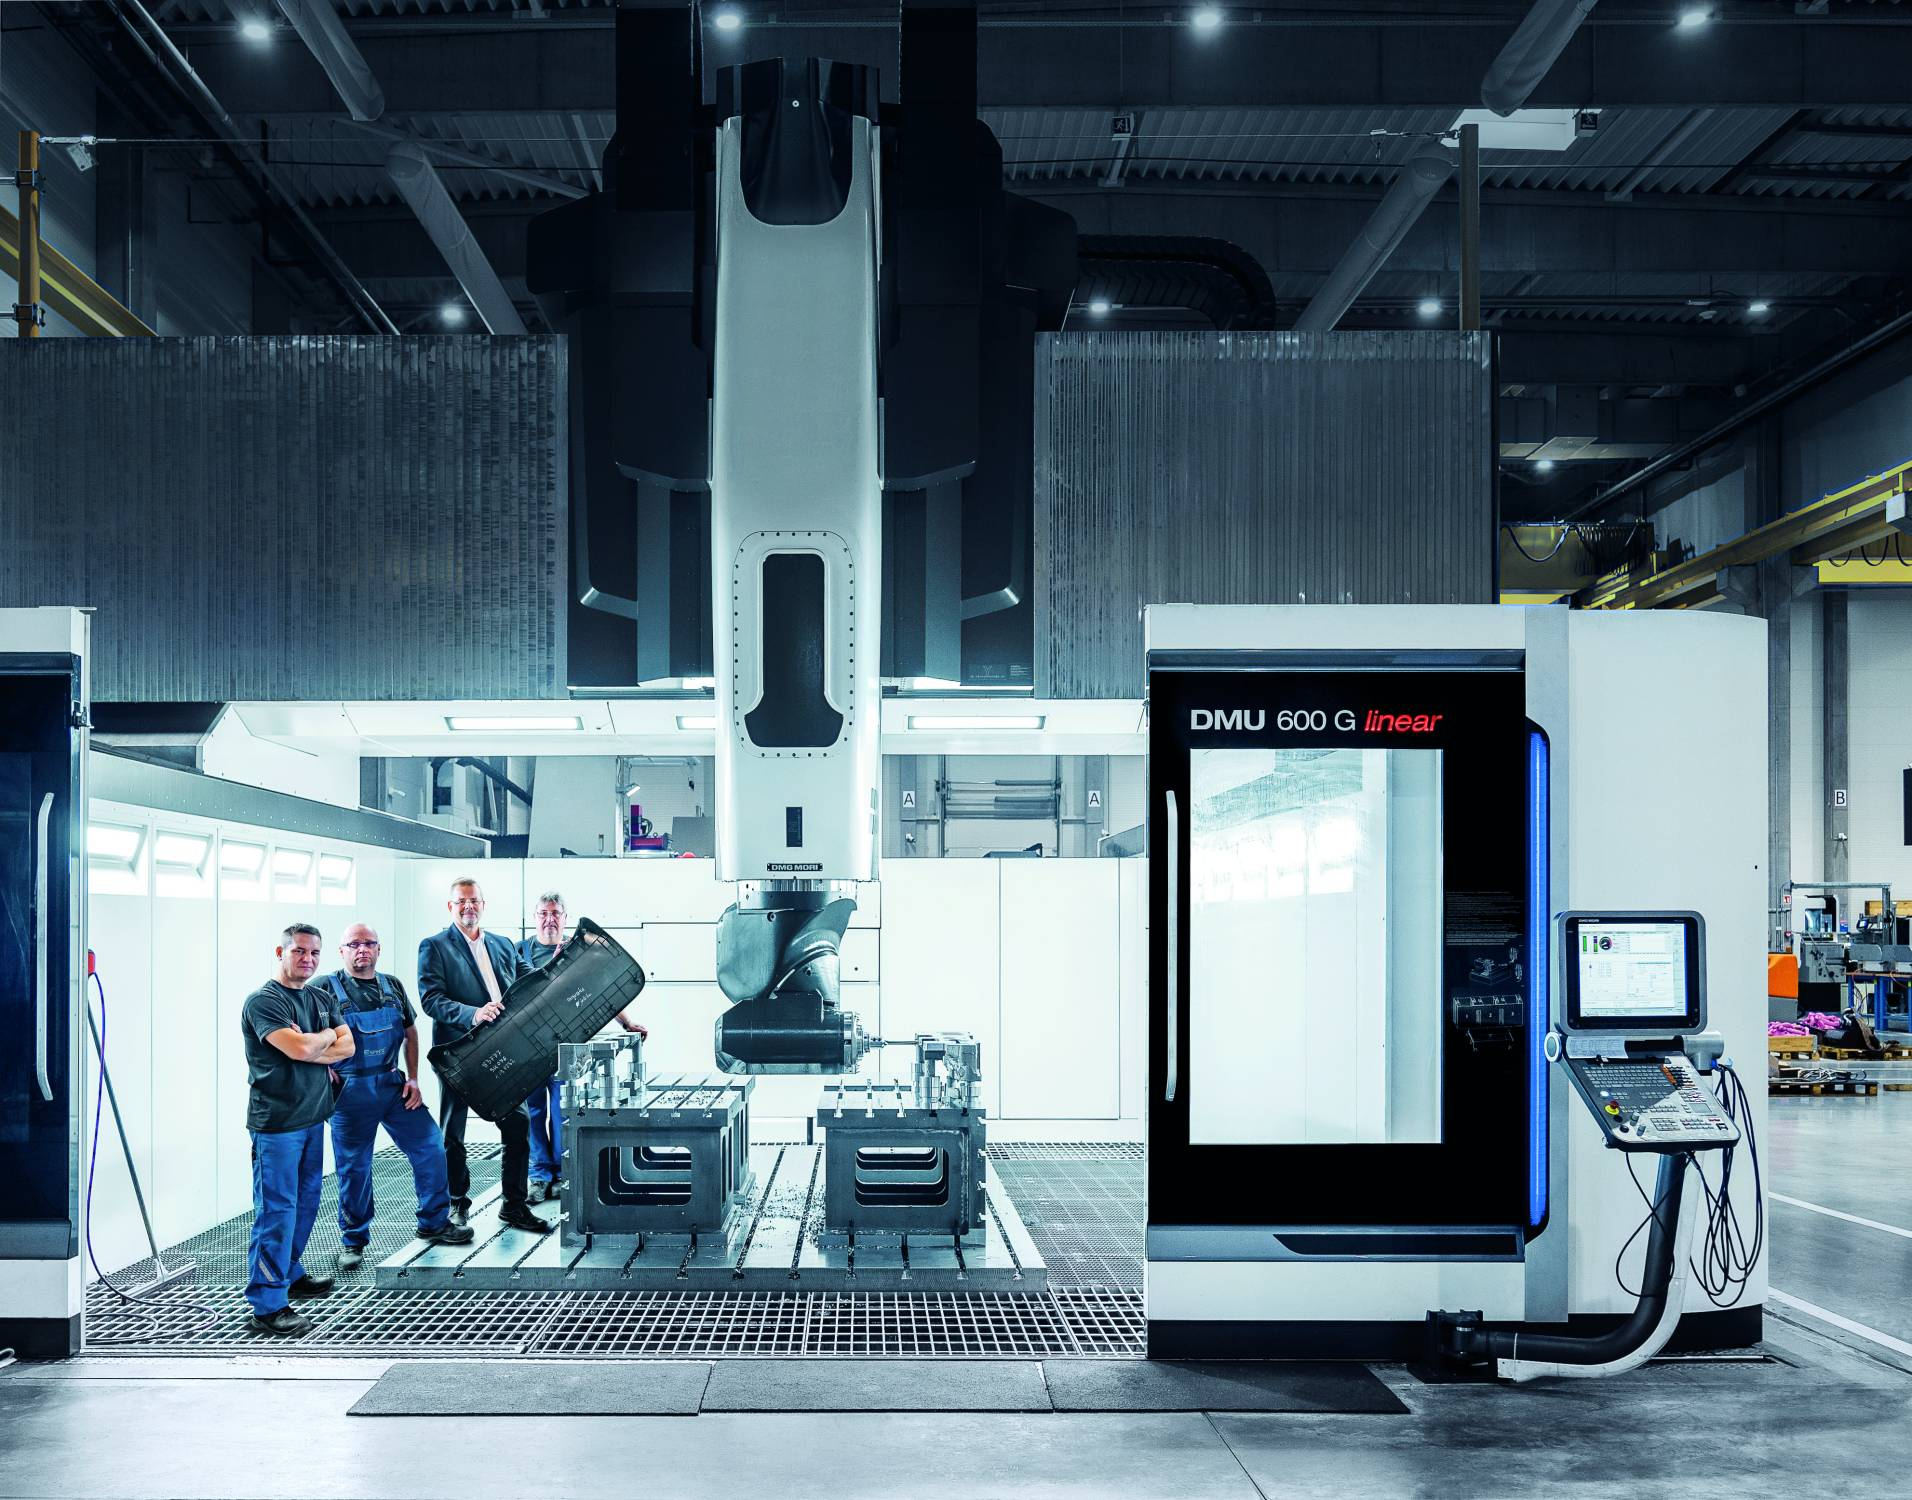
\includegraphics[width=\linewidth,height=5.20833in,keepaspectratio]{images-1/dmu600p.jpg}

}

\caption{DMG Mori DMU600p linear}

\end{figure}%

\subsection{Parameters}\label{parameters-1}

\begin{itemize}
\tightlist
\item
  Axes configuration
\item
  Axes travels
\item
  Spindle speed
\item
  Rapid speed
\item
  Spindle torque and power
\end{itemize}

\begin{figure}[H]

{\centering 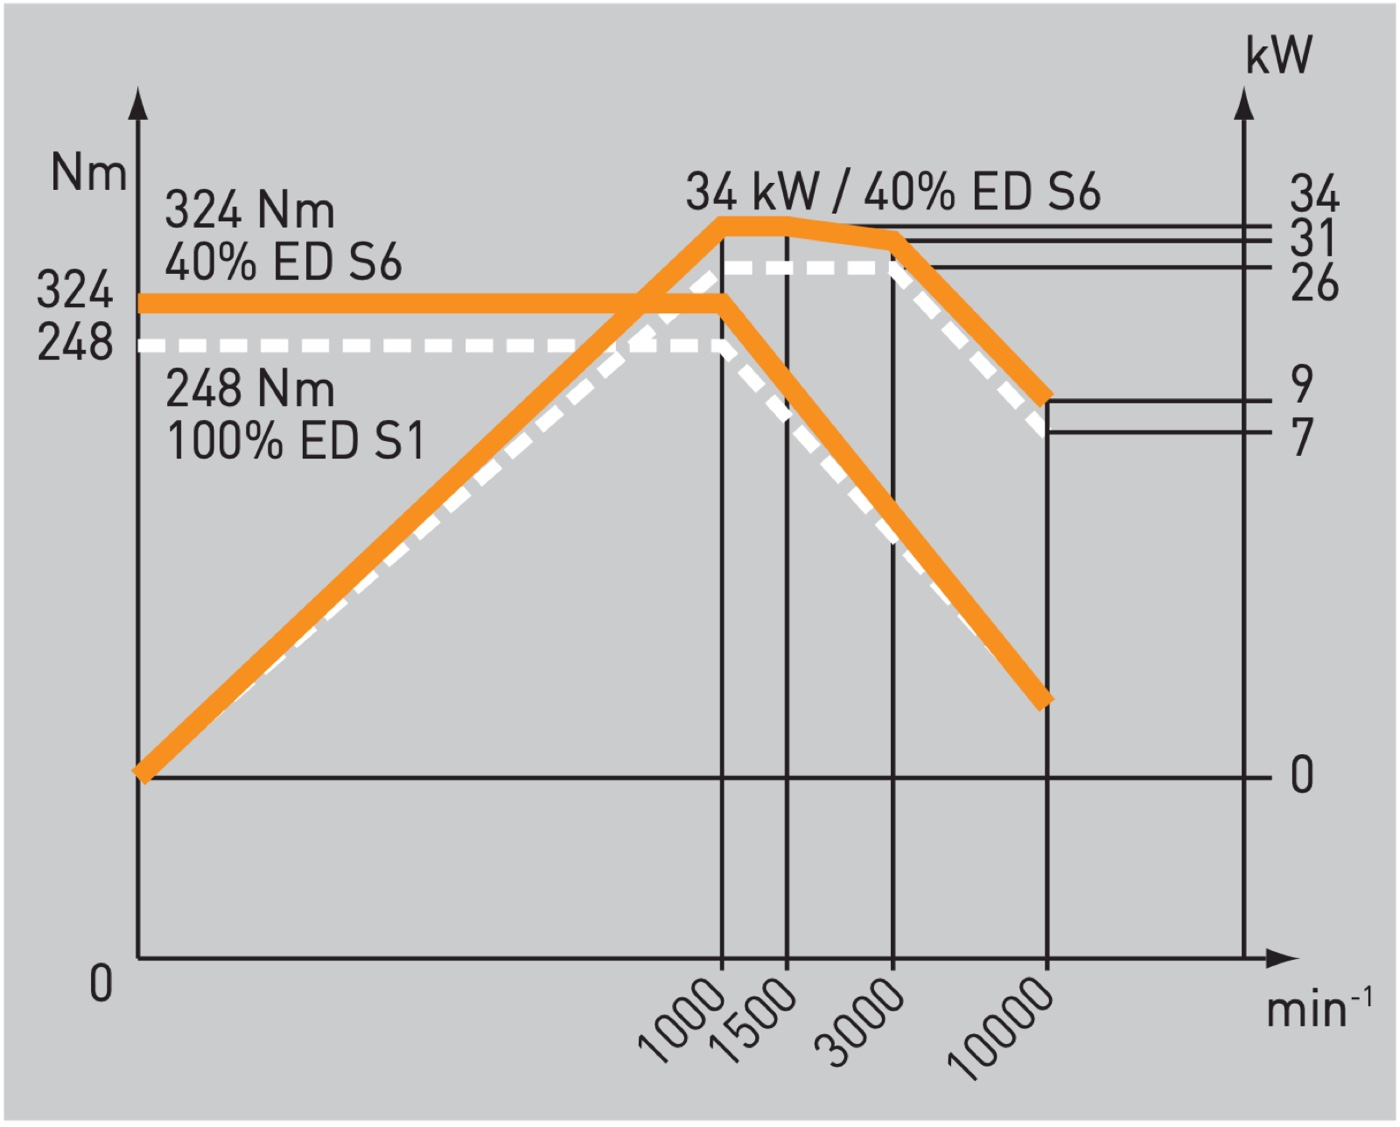
\includegraphics[width=0.8\linewidth,height=\textheight,keepaspectratio]{images/spindle-power.jpg}

}

\caption{ED = \emph{Einschaltdauer} (operating time)}

\end{figure}%

\section{Automation}\label{automation}

\emph{It is mainly a matter of synchronizing motion}

\begin{center}
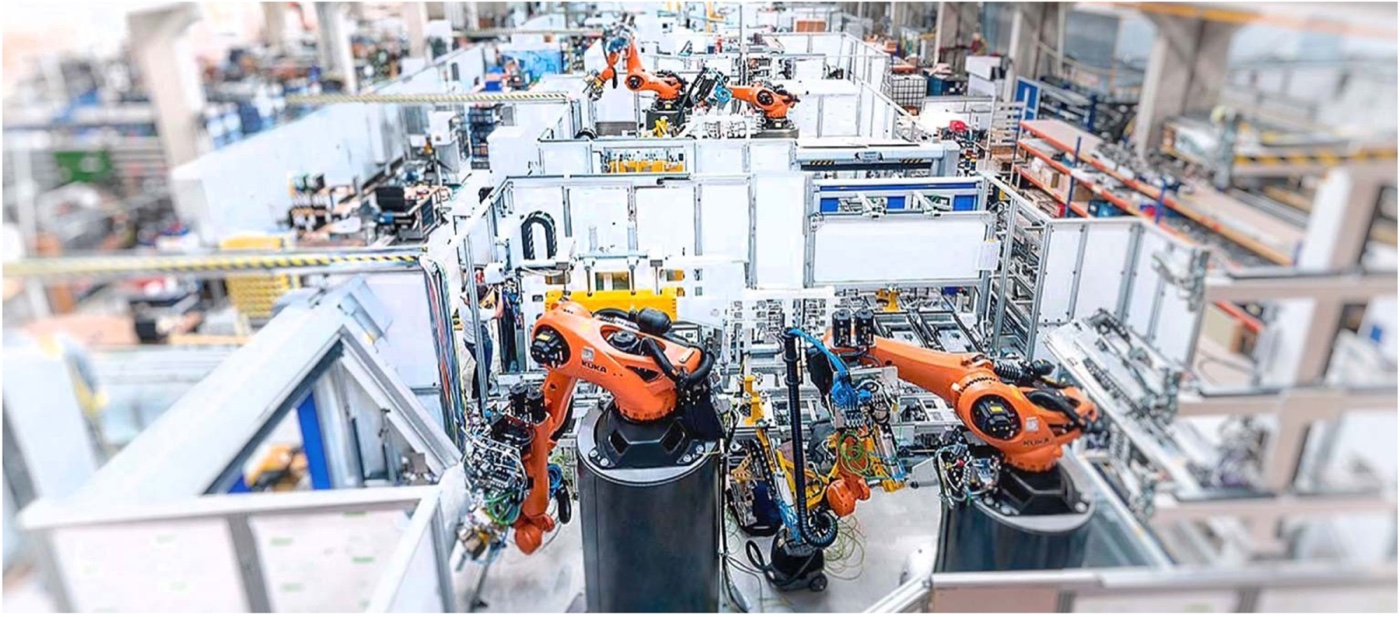
\includegraphics[width=\linewidth,height=3.33333in,keepaspectratio]{images/automation-photo.jpg}
\end{center}

\subsection{Amber \& Amber}\label{amber-amber}

\emph{The Yardstick of Automation} (1962)

{\def\LTcaptype{none} % do not increment counter
\begin{longtable}[]{@{}
  >{\centering\arraybackslash}p{(\linewidth - 4\tabcolsep) * \real{0.3333}}
  >{\centering\arraybackslash}p{(\linewidth - 4\tabcolsep) * \real{0.3333}}
  >{\raggedright\arraybackslash}p{(\linewidth - 4\tabcolsep) * \real{0.3333}}@{}}
\toprule\noalign{}
\begin{minipage}[b]{\linewidth}\centering
Order
\end{minipage} & \begin{minipage}[b]{\linewidth}\centering
Human attribute
\end{minipage} & \begin{minipage}[b]{\linewidth}\raggedright
Example
\end{minipage} \\
\midrule\noalign{}
\endhead
\bottomrule\noalign{}
\endlastfoot
0 & None & Utensili manuali \\
1 & Energy & Powered machines and tools \\
2 & Dexterity & Single-cycle automatics (\emph{dexterity =
self-feeding}) \\
3 & Diligence & Repeats cycle; open-loop control \\
4 & Judgment & Closed loop; numerical control; self-measuring \\
5 & Evaluation & Computer control; model of process required for
automation \\
6 & Learning & Limited self-programming; some artificial intelligence \\
7 & Reasoning & Inductive reasoning (cause-effects) \\
8 & Creativity & Performs (original) design unaided \\
9 & Dominance & Machine is master (HAL 9000) \\
\end{longtable}
}

\subsection{Current level: A(4)}\label{current-level-a4}

\begin{itemize}
\tightlist
\item
  CNC machine tools

  \begin{itemize}
  \tightlist
  \item
    Convert a machining description in machining movements
  \item
    Run machining commands with \emph{judgement} (A4)
  \end{itemize}
\end{itemize}

\begin{center}
\includegraphics[width=\linewidth,height=4.47917in,keepaspectratio]{1-machine_tools_files/mediabag/images-1/cnc-block-diagram.pdf}
\end{center}

\subsection{Machine tool elements}\label{machine-tool-elements}

\begin{center}
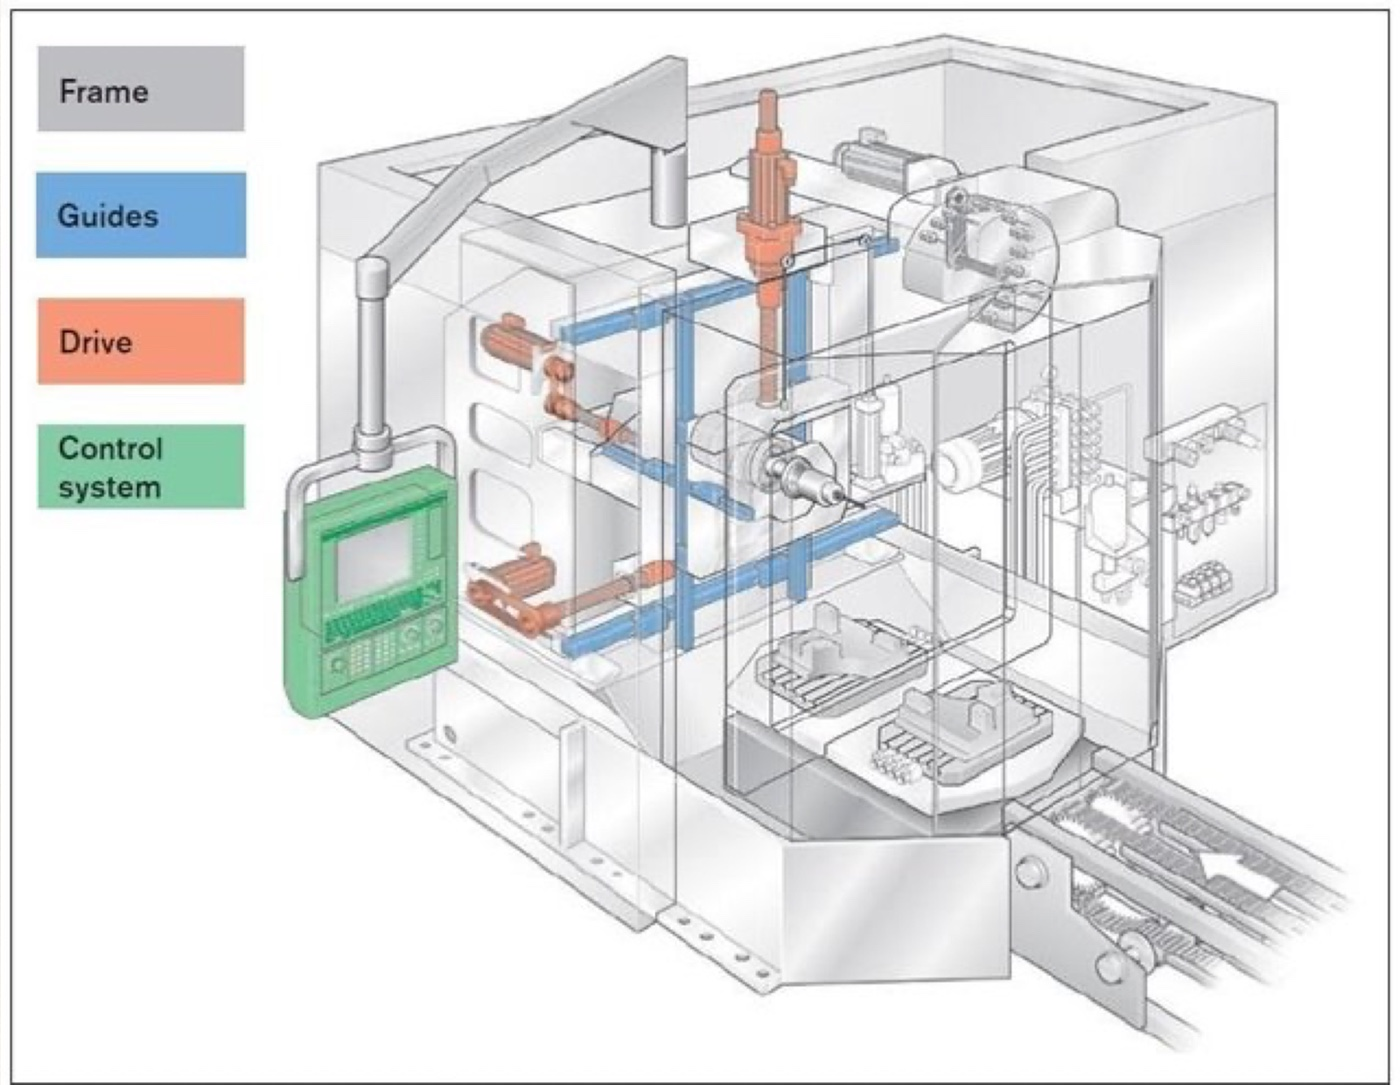
\includegraphics[width=\linewidth,height=4.89583in,keepaspectratio]{images/mt-elements.jpg}
\end{center}

\subsection{}\label{section}

\subsection{Drivers}\label{drivers}

\begin{center}
\includegraphics[width=\linewidth,height=1.45833in,keepaspectratio]{1-machine_tools_files/mediabag/images-1/driver-loop.pdf}
\end{center}

Requirements:

\begin{itemize}
\tightlist
\item
  Fast response (acceleration)
\item
  Quick stabilization (minimum number of oscillations)
\item
  \textbf{No overshoot} (or risk of damages)
\end{itemize}

\subsection{Feedback}\label{feedback}

\begin{figure}[H]

{\centering \includegraphics[width=\linewidth,height=4.89583in,keepaspectratio]{1-machine_tools_files/mediabag/images-1/feedback-loops.pdf}

}

\caption{Open loop (A3); closed loop on motor, on lead screw, on axis
(A4)}

\end{figure}%

\subsection{Errors}\label{errors}

\begin{center}
\includegraphics[width=\linewidth,height=2.60417in,keepaspectratio]{1-machine_tools_files/mediabag/images-1/errors-diagram.pdf}
\end{center}

\begin{center}
\includegraphics[width=\linewidth,height=2.08333in,keepaspectratio]{1-machine_tools_files/mediabag/images-1/drive-1.pdf}
\end{center}

\begin{center}
\includegraphics[width=\linewidth,height=2.08333in,keepaspectratio]{1-machine_tools_files/mediabag/images-1/drive-2.pdf}
\end{center}

\subsection{Linear axis control}\label{linear-axis-control}

\begin{center}
\includegraphics[width=\linewidth,height=4.47917in,keepaspectratio]{1-machine_tools_files/mediabag/images-1/linear-axis.pdf}
\end{center}

Encoder gain: pulses/rev --- Axis gain: screw pitch × encoder gain
(mm/pulse)

\subsection{}\label{section-1}

\subsection{Linear guide-rail}\label{linear-guide-rail}

\begin{center}
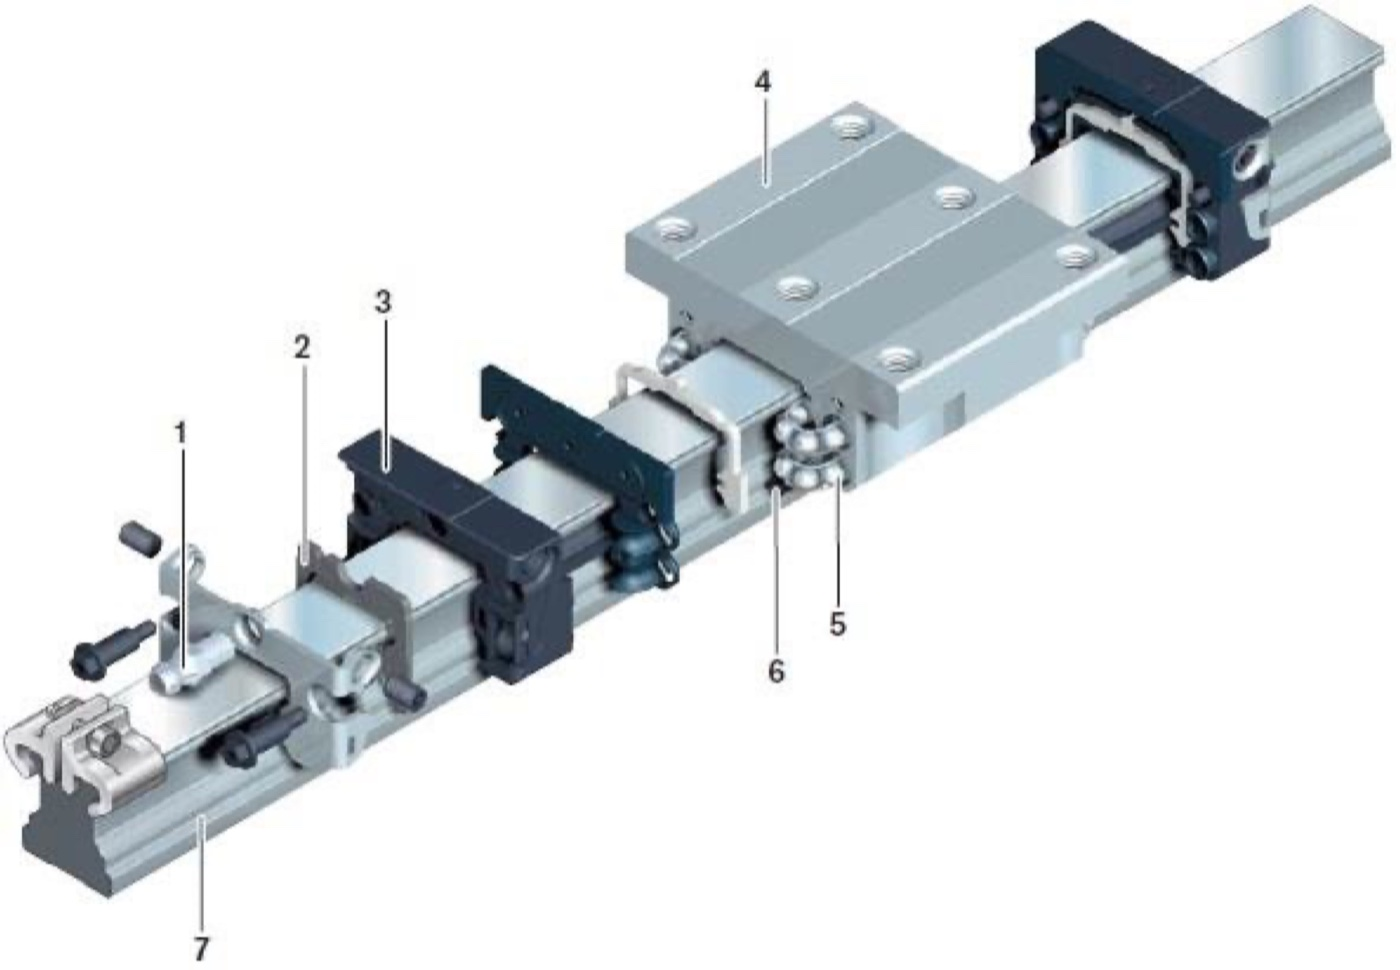
\includegraphics[width=\linewidth,height=3.95833in,keepaspectratio]{images/guide-rail.jpg}
\end{center}

\begin{enumerate}
\def\labelenumi{\arabic{enumi}.}
\tightlist
\item
  Lube port
\item
  end wiper seal
\item
  end cap
\item
  runner block body
\item
  rolling element
\item
  side seal
\item
  guide rail
\end{enumerate}

\subsection{Encoder}\label{encoder}

\begin{itemize}
\tightlist
\item
  \textbf{Types}

  \begin{itemize}
  \tightlist
  \item
    Rotary encoders
  \item
    Linear encoders
  \end{itemize}
\item
  \textbf{Quality}

  \begin{itemize}
  \tightlist
  \item
    Incremental
  \item
    Absolute (Gray code)
  \end{itemize}
\end{itemize}

\subsection{PID controllers}\label{pid-controllers}

\begin{center}
\includegraphics[width=\linewidth,height=2.60417in,keepaspectratio]{1-machine_tools_files/mediabag/images-1/pid-diagram.pdf}
\end{center}

{\def\LTcaptype{none} % do not increment counter
\begin{longtable}[]{@{}
  >{\centering\arraybackslash}p{(\linewidth - 10\tabcolsep) * \real{0.1667}}
  >{\centering\arraybackslash}p{(\linewidth - 10\tabcolsep) * \real{0.1667}}
  >{\centering\arraybackslash}p{(\linewidth - 10\tabcolsep) * \real{0.1667}}
  >{\centering\arraybackslash}p{(\linewidth - 10\tabcolsep) * \real{0.1667}}
  >{\centering\arraybackslash}p{(\linewidth - 10\tabcolsep) * \real{0.1667}}
  >{\centering\arraybackslash}p{(\linewidth - 10\tabcolsep) * \real{0.1667}}@{}}
\toprule\noalign{}
\begin{minipage}[b]{\linewidth}\centering
Parameter
\end{minipage} & \begin{minipage}[b]{\linewidth}\centering
Rise time
\end{minipage} & \begin{minipage}[b]{\linewidth}\centering
Overshoot
\end{minipage} & \begin{minipage}[b]{\linewidth}\centering
Settling time
\end{minipage} & \begin{minipage}[b]{\linewidth}\centering
Steady-state error
\end{minipage} & \begin{minipage}[b]{\linewidth}\centering
Stability
\end{minipage} \\
\midrule\noalign{}
\endhead
\bottomrule\noalign{}
\endlastfoot
\textbf{Kp} & Decrease & Increase & Small change & Decrease & Degrade \\
\textbf{Ki} & Decrease & Increase & Increase & Decrease significantly &
Degrade \\
\textbf{Kd} & Minor decrease & Minor decrease & Minor decrease & No
effect & Improve if Kd small \\
\end{longtable}
}

\subsection{Actual control schemes}\label{actual-control-schemes}

\begin{center}
\includegraphics[width=\linewidth,height=2.91667in,keepaspectratio]{1-machine_tools_files/mediabag/images-1/control-schemes-a.pdf}
\end{center}

\begin{center}
\includegraphics[width=\linewidth,height=2.5in,keepaspectratio]{1-machine_tools_files/mediabag/images-1/control-schemes-b.pdf}
\end{center}

\subsection{PLC: Programmable Logic
Controller}\label{plc-programmable-logic-controller}

PLC is a controller that implements logic relationships between inputs
and outputs. It provides a range of interfaces and registers:

\begin{itemize}
\tightlist
\item
  Analog and digital I/O (\textgreater{} 2048)
\item
  Relay (1000)
\item
  Memories (200)
\item
  Timers (200)
\item
  Counters (200)
\end{itemize}

\begin{center}
\includegraphics[width=\linewidth,height=4.47917in,keepaspectratio]{1-machine_tools_files/mediabag/images-1/cnc-block-diagram.pdf}
\end{center}

\begin{tcolorbox}[enhanced jigsaw, arc=.35mm, bottomrule=.15mm, bottomtitle=1mm, breakable, colback=white, colbacktitle=quarto-callout-note-color!10!white, colframe=quarto-callout-note-color-frame, coltitle=black, left=2mm, leftrule=.75mm, opacityback=0, opacitybacktitle=0.6, rightrule=.15mm, title=\textcolor{quarto-callout-note-color}{\faInfo}\hspace{0.5em}{Note}, titlerule=0mm, toprule=.15mm, toptitle=1mm]

Can be either a separate hardware, or a software process running on the
same computer that runs the CNC

\end{tcolorbox}

\subsection{PLC}\label{plc}

\begin{itemize}
\tightlist
\item
  Beside GPIO, PLC can also have advanced I/O and communication
  capabilities:

  \begin{itemize}
  \tightlist
  \item
    General purpose communication: RS232, RS422, Ethernet
  \item
    Deterministic communication: Profibus, DeviceNet, Modbus, Industrial
    EtherNET, CAN-BUS
  \item
    Special I/O: counters, virtual cams, PIDs and controllers
  \end{itemize}
\item
  PLC programming languages have been designed to facilitate the
  transition from \textbf{wired logics} to \textbf{software logics}: the
  languages had to be intuitive and immediately productive for
  technicians with different backgrounds: \textbf{electrical
  engineering}, control engineering, firmware programming
\end{itemize}

\subsection{PLC}\label{plc-1}

The programming standard \textbf{IEC 61131-3} provided this transition:

{\def\LTcaptype{none} % do not increment counter
\begin{longtable}[]{@{}
  >{\raggedright\arraybackslash}p{(\linewidth - 4\tabcolsep) * \real{0.2941}}
  >{\centering\arraybackslash}p{(\linewidth - 4\tabcolsep) * \real{0.1765}}
  >{\raggedright\arraybackslash}p{(\linewidth - 4\tabcolsep) * \real{0.5294}}@{}}
\toprule\noalign{}
\begin{minipage}[b]{\linewidth}\raggedright
Language
\end{minipage} & \begin{minipage}[b]{\linewidth}\centering
Type
\end{minipage} & \begin{minipage}[b]{\linewidth}\raggedright
Description
\end{minipage} \\
\midrule\noalign{}
\endhead
\bottomrule\noalign{}
\endlastfoot
Ladder Logic & Graphical & Resembles relay logic diagrams, intuitive for
electricians \\
Function Block Diagram & Graphical & Resembles block diagrams, intuitive
for control engineers \\
Sequential Function Chart & Graphical & Resembles flow charts and
\href{https://en.wikipedia.org/wiki/Finite-state_machine}{finite state
machines}, intuitive for process engineers \\
Structured Text & Textual & Resembles Pascal, intuitive for software
engineers \\
Instruction List & Textual & Resembles assembly, intuitive for firmware
engineers \\
\end{longtable}
}

\begin{tcolorbox}[enhanced jigsaw, arc=.35mm, bottomrule=.15mm, bottomtitle=1mm, breakable, colback=white, colbacktitle=quarto-callout-note-color!10!white, colframe=quarto-callout-note-color-frame, coltitle=black, left=2mm, leftrule=.75mm, opacityback=0, opacitybacktitle=0.6, rightrule=.15mm, title=\textcolor{quarto-callout-note-color}{\faInfo}\hspace{0.5em}{Note}, titlerule=0mm, toprule=.15mm, toptitle=1mm]

The standard states that languages must be interchangeable, i.e., the
same program can be written in any language and must have the same
behavior, different parts of a program can be written in different
languages, and the program can be converted from one language to another

\end{tcolorbox}

\subsection{PLC: Ladder diagram}\label{plc-ladder-diagram}

\begin{tcolorbox}[enhanced jigsaw, arc=.35mm, bottomrule=.15mm, bottomtitle=1mm, breakable, colback=white, colbacktitle=quarto-callout-note-color!10!white, colframe=quarto-callout-note-color-frame, coltitle=black, left=2mm, leftrule=.75mm, opacityback=0, opacitybacktitle=0.6, rightrule=.15mm, title=\textcolor{quarto-callout-note-color}{\faInfo}\hspace{0.5em}{Note}, titlerule=0mm, toprule=.15mm, toptitle=1mm]

\begin{itemize}
\tightlist
\item
  On the left side there are \textbf{contactors} (inputs), on the right
  side there are \textbf{coils} (outputs).
\item
  parallel branches represent \textbf{OR} logic, series branches
  represent \textbf{AND} logic; contactors can be \textbf{normally open}
  or \textbf{normally closed} (\textbf{NOT}).
\item
  The program is read from left to right, top to bottom. The program is
  executed in a \textbf{cyclic scan}: all inputs are read, the logic is
  evaluated, and the outputs are updated.
\end{itemize}

\end{tcolorbox}

\begin{center}
\includegraphics[width=\linewidth,height=4.89583in,keepaspectratio]{1-machine_tools_files/mediabag/images-1/plc-ladder.pdf}
\end{center}

\subsection{PLC: Function Block
Diagram}\label{plc-function-block-diagram}

\begin{tcolorbox}[enhanced jigsaw, arc=.35mm, bottomrule=.15mm, bottomtitle=1mm, breakable, colback=white, colbacktitle=quarto-callout-note-color!10!white, colframe=quarto-callout-note-color-frame, coltitle=black, left=2mm, leftrule=.75mm, opacityback=0, opacitybacktitle=0.6, rightrule=.15mm, title=\textcolor{quarto-callout-note-color}{\faInfo}\hspace{0.5em}{Note}, titlerule=0mm, toprule=.15mm, toptitle=1mm]

\begin{itemize}
\tightlist
\item
  Each block implements a function, which can be a logic function, a
  timer, a counter, or even a more complicated one as a PID controller
\item
  Appeals to control engineers, being quite similar to
  \href{https://www.mathworks.com/products/simulink.html}{Simulink} and
  other block-diagram-based control design software
\item
  Complex programs tend to become quite messy, so FBD is often used in
  combination with other languages and limited to implement specific
  functions related to control and signal processing
\end{itemize}

\end{tcolorbox}

\begin{center}
\includegraphics[width=\linewidth,height=4.89583in,keepaspectratio]{1-machine_tools_files/mediabag/images-1/plc-fbd.pdf}
\end{center}

\subsection{PLC: Sequential Function
Chart}\label{plc-sequential-function-chart}

\begin{tcolorbox}[enhanced jigsaw, arc=.35mm, bottomrule=.15mm, bottomtitle=1mm, breakable, colback=white, colbacktitle=quarto-callout-note-color!10!white, colframe=quarto-callout-note-color-frame, coltitle=black, left=2mm, leftrule=.75mm, opacityback=0, opacitybacktitle=0.6, rightrule=.15mm, title=\textcolor{quarto-callout-note-color}{\faInfo}\hspace{0.5em}{Note}, titlerule=0mm, toprule=.15mm, toptitle=1mm]

\begin{itemize}
\tightlist
\item
  SFC is a graphical language that implements a \textbf{finite state
  machine}
\item
  Each block is a \textbf{state}, each line a transition with its
  activation condition
\item
  It is very intuitive for process engineers, and it is often used in
  combination with other languages to implement the \textbf{overall
  logic} of a process, while the other languages are used to implement
  the \textbf{details} of each state
\end{itemize}

\end{tcolorbox}

\begin{center}
\includegraphics[width=\linewidth,height=4.89583in,keepaspectratio]{1-machine_tools_files/mediabag/images-1/plc-sfc.pdf}
\end{center}

\subsection{PLC: Textual languages}\label{plc-textual-languages}

\begin{codelisting}

\caption{\texttt{Structured Text (ST)}}

\begin{Shaded}
\begin{Highlighting}[]
\CommentTok{(* motor start/stop with seal{-}in *)}
\NormalTok{Motor := (Start\_PB }\KeywordTok{OR}\NormalTok{ Motor)}
         \KeywordTok{AND} \KeywordTok{NOT}\NormalTok{ Stop\_PB}
         \KeywordTok{AND} \KeywordTok{NOT}\NormalTok{ Overload;}
\NormalTok{Inlet\_Valve := Motor }\KeywordTok{AND} \KeywordTok{NOT}\NormalTok{ Level\_Hi;}
\NormalTok{T1(}\KeywordTok{IN}\NormalTok{ := Motor, PT := T}\StringTok{\#10s)}\NormalTok{;}
\KeywordTok{IF}\NormalTok{ T1.Q }\KeywordTok{THEN}
\NormalTok{  Run\_Lamp := }\KeywordTok{TRUE}\NormalTok{;}
\NormalTok{END\_IF;}
\end{Highlighting}
\end{Shaded}

\end{codelisting}

\begin{codelisting}

\caption{\texttt{Instruction List (IL)}}

\begin{Shaded}
\begin{Highlighting}[]
\NormalTok{LD   Start\_PB}
\BuiltInTok{OR}\NormalTok{   Motor}
\BuiltInTok{ANDN}\NormalTok{ Stop\_PB}
\BuiltInTok{ANDN}\NormalTok{ Overload}
\NormalTok{ST   Motor}
\NormalTok{LD   Motor}
\BuiltInTok{ANDN}\NormalTok{ Level\_Hi}
\NormalTok{ST   Inlet\_Valve}
\NormalTok{CAL  T1}\OperatorTok{(}\NormalTok{IN }\OperatorTok{:=}\NormalTok{ Motor}\OperatorTok{,}\NormalTok{ PT }\OperatorTok{:=}\NormalTok{ T}\OperatorTok{\#}\DecValTok{10}\ErrorTok{s}\OperatorTok{)}
\NormalTok{LD   T1}\OperatorTok{.}\NormalTok{Q}
\NormalTok{S    Run\_Lamp}
\end{Highlighting}
\end{Shaded}

\end{codelisting}

\begin{tcolorbox}[enhanced jigsaw, arc=.35mm, bottomrule=.15mm, bottomtitle=1mm, breakable, colback=white, colbacktitle=quarto-callout-note-color!10!white, colframe=quarto-callout-note-color-frame, coltitle=black, left=2mm, leftrule=.75mm, opacityback=0, opacitybacktitle=0.6, rightrule=.15mm, title=\textcolor{quarto-callout-note-color}{\faInfo}\hspace{0.5em}{Note}, titlerule=0mm, toprule=.15mm, toptitle=1mm]

Textual languages are the most easy to implement and always available
even on low-cost PLC and PLC IDEs

\end{tcolorbox}

\subsection{(Computer) Numerical
Control}\label{computer-numerical-control}

The CNC controller is the \textbf{brain} of the machine tool. It
implements the \textbf{judgement} (A4) of Amber's scale, and it is
responsible for:

\begin{itemize}
\tightlist
\item
  parsing the \textbf{part-program}
\item
  converting it into \textbf{motion commands} for the machine tool
  actuators
\item
  providing action inputs to the \textbf{PLC controller} for auxiliary
  functions (coolant, tool change routines, etc.)
\end{itemize}

CNC controllers are characterized by:

\begin{itemize}
\tightlist
\item
  Types of \textbf{motion interpolation}
\item
  Number of \textbf{controlled axes}
\end{itemize}

\subsection{Types of motion
interpolation}\label{types-of-motion-interpolation}

CNC can control axes with increasing levels of sophistication:

\begin{itemize}
\tightlist
\item
  \textbf{Point to point}: only the start and end points are controlled,
  the path is not controlled (drilling, pick-and-place)
\item
  \textbf{Paraxial}: one axis at a time can be \textbf{controlled in
  feed} (semi-automatic machines, machines that don't need axes
  interpolation as sawing machines, presses)
\item
  {Continuous}: all axes can be controlled simultaneously, and the path
  is controlled in position and velocity
\end{itemize}

\subsection{Number of controlled axes}\label{number-of-controlled-axes}

\begin{itemize}
\tightlist
\item
  2 Axes: third axis is manually adjusted (manual lathes, manual mills)
\item
  2 Axes and 1/2: only two axes at a time can be controlled, the third
  is for positioning
\item
  3 Axes: full 3-D trajectory control of TCP
\item
  5 Axes: full trajectory control of TCP and tool orientation
\end{itemize}

\subsection{Coordinate systems}\label{coordinate-systems}

\begin{itemize}
\tightlist
\item
  Axes references combine to give machine origin
\item
  Axes references are used to reset encoders (\emph{homing})
\item
  Machine controller works in \textbf{machine coordinates}
\item
  Workpiece origin is \textbf{set up by the operator}
\item
  Registration point is the reference to measure tool length and
  diameter
\item
  Support point is the reference to mount the tool on the spindle (when
  mounted, \emph{reference = support})
\end{itemize}

{\def\LTcaptype{none} % do not increment counter
\begin{longtable}[]{@{}
  >{\raggedright\arraybackslash}p{(\linewidth - 2\tabcolsep) * \real{0.7500}}
  >{\centering\arraybackslash}p{(\linewidth - 2\tabcolsep) * \real{0.2500}}@{}}
\toprule\noalign{}
\begin{minipage}[b]{\linewidth}\raggedright
Reference
\end{minipage} & \begin{minipage}[b]{\linewidth}\centering
Symbol
\end{minipage} \\
\midrule\noalign{}
\endhead
\bottomrule\noalign{}
\endlastfoot
Axis reference & \begin{center}

\includegraphics[width=\linewidth,height=0.3125in,keepaspectratio]{images-1/axis-reference.png}
\end{center}
 \\
Machine origin & \begin{center}
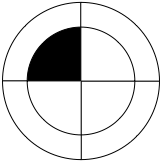
\includegraphics[width=\linewidth,height=0.3125in,keepaspectratio]{images-1/machine-origin.png}
\end{center}
 \\
Workpiece origin & \begin{center}
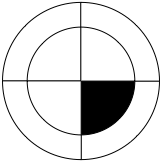
\includegraphics[width=\linewidth,height=0.3125in,keepaspectratio]{images-1/wp-origin.png}
\end{center}
 \\
Registration point & \begin{center}
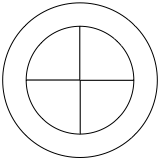
\includegraphics[width=\linewidth,height=0.3125in,keepaspectratio]{images-1/registration-point.png}
\end{center}
 \\
Support point & \begin{center}

\includegraphics[width=\linewidth,height=0.3125in,keepaspectratio]{images-1/support-point.png}
\end{center}
 \\
\end{longtable}
}

\subsection{Tool reference}\label{tool-reference}

\begin{itemize}
\tightlist
\item
  \textbf{Support point:}

  \begin{itemize}
  \tightlist
  \item
    Abutment plane (lathes)
  \item
    Spindle nose (mills)
  \end{itemize}
\item
  \textbf{Registration point:}

  \begin{itemize}
  \tightlist
  \item
    on the tool, the point that matches the SP when mounted
  \end{itemize}
\item
  \textbf{To be measured:}

  \begin{itemize}
  \tightlist
  \item
    Length and offset (lathes)
  \item
    Length, diameter, and toric radius (mills)
  \end{itemize}
\end{itemize}

\begin{center}
\includegraphics[width=\linewidth,height=4.6875in,keepaspectratio]{1-machine_tools_files/mediabag/images-1/tool-ref.pdf}
\end{center}

\subsection{WP coordinates}\label{wp-coordinates}

\begin{itemize}
\tightlist
\item
  Selected by operator/programmer
\item
  Part program can use WP coordinates and/or machine coordinates
\item
  After fixturing, WP origin has to be set up wrt machine origin

  \begin{itemize}
  \tightlist
  \item
    by touching with tool and compensating for tool radius
  \item
    By 3-D touch probe
  \end{itemize}
\end{itemize}

\subsection{Coordinate
transformations}\label{coordinate-transformations}

\begin{itemize}
\tightlist
\item
  The part program defines the toolpath as the trajectory of the
  \textbf{tool center position} (TCP) in the workpiece reference frame
\item
  The CNC controller converts the TCP coordinates into \textbf{machine
  coordinates} by applying a roto-translation transformation that
  accounts for:

  \begin{itemize}
  \tightlist
  \item
    the workpiece origin
  \item
    the tool length
  \end{itemize}
\item
  Tool diameter is accounted for by the \textbf{tool radius
  compensation} function, which offsets the toolpath by the tool radius
  in a direction perpendicular to the toolpath
\end{itemize}

\begin{tcolorbox}[enhanced jigsaw, arc=.35mm, bottomrule=.15mm, bottomtitle=1mm, breakable, colback=white, colbacktitle=quarto-callout-note-color!10!white, colframe=quarto-callout-note-color-frame, coltitle=black, left=2mm, leftrule=.75mm, opacityback=0, opacitybacktitle=0.6, rightrule=.15mm, title=\textcolor{quarto-callout-note-color}{\faInfo}\hspace{0.5em}{Note}, titlerule=0mm, toprule=.15mm, toptitle=1mm]

In turning, there is no tool radius compensation; rather, tool is
measured by \textbf{length} and \textbf{abutment}, the latter being the
offset w.r.t. the registration point

\end{tcolorbox}

\subsection{Coordinate
transformations}\label{coordinate-transformations-1}

Any coordinate \(P_{wp}\) given in the workpiece reference frame
\(O_{wp}\) is converted in machine coordinates \(P_m\), including tool
length offset

\[
P_m = T_{wp \to m} P_{wp}; \qquad
T_{wp \to m} = \begin{bmatrix} r_{11} & r_{12} & r_{13} & d_x \\ r_{21} & r_{22} & r_{23} & d_y \\ r_{31} & r_{32} & r_{33} & d_z + l_t \\ 0 & 0 & 0 & 1 \end{bmatrix}
\]

\(d_{x-z}\) are coordinates of \(O_{wp}\) in \(O_m\)

\begin{center}
\includegraphics[width=\linewidth,height=3.4375in,keepaspectratio]{1-machine_tools_files/mediabag/images-1/transform-3d.pdf}
\end{center}

\subsection{Coordinate
transformations}\label{coordinate-transformations-2}

Remember that the roto-translation matrix is:

\[
T = \begin{bmatrix}
\cos\alpha\cos\beta & \cos\alpha\sin\beta\sin\gamma - \sin\alpha\cos\beta & \cos\alpha\sin\beta\cos\gamma + \sin\alpha\sin\gamma & d_x \\
\sin\alpha\cos\beta & \sin\alpha\sin\beta\sin\gamma + \cos\alpha\cos\beta & \sin\alpha\sin\beta\cos\gamma - \cos\alpha\sin\gamma & d_y \\
-\sin\beta & \cos\beta\sin\gamma & \cos\beta\cos\gamma & d_z \\
0 & 0 & 0 & 1
\end{bmatrix}
\]

The \textbf{order of transformations} is:

\begin{enumerate}
\def\labelenumi{\arabic{enumi}.}
\tightlist
\item
  Roll by \(\gamma\)
\item
  Pitch by \(\beta\)
\item
  Yaw by \(\alpha\)
\item
  Translate by \((d_x, d_y, d_z)\)
\end{enumerate}

\begin{center}
\includegraphics[width=\linewidth,height=2.39583in,keepaspectratio]{1-machine_tools_files/mediabag/images-1/rpy.pdf}
\end{center}

\subsection{Coordinate transformations (3-axes
machines)}\label{coordinate-transformations-3-axes-machines}

Machines with 3 controlled axes (no tool alignment) typically implement
a simplified transformation that only accounts for the workpiece origin
translation and rotation \(\theta\) about \(z\) and tool length:

\[
\begin{bmatrix} x_m \\ y_m \\ z_m \\1 \end{bmatrix} =
\begin{bmatrix} \cos\theta & -\sin\theta & 0 & d_x \\
\sin\theta & \cos\theta & 0 & d_y \\
0 & 0 & 1 & d_z + l_t \\
0 & 0 & 0 & 1 \end{bmatrix}
\begin{bmatrix} x \\ y \\ z \\ 1 \end{bmatrix}
\]

\begin{tcolorbox}[enhanced jigsaw, arc=.35mm, bottomrule=.15mm, bottomtitle=1mm, breakable, colback=white, colbacktitle=quarto-callout-tip-color!10!white, colframe=quarto-callout-tip-color-frame, coltitle=black, left=2mm, leftrule=.75mm, opacityback=0, opacitybacktitle=0.6, rightrule=.15mm, title=\textcolor{quarto-callout-tip-color}{\faLightbulb}\hspace{0.5em}{Workplane tilt compensation}, titlerule=0mm, toprule=.15mm, toptitle=1mm]

Even for 3 axes machines, it is customary to also include \textbf{small}
rotations about \(x\) and \(y\) in the transformation matrix, to account
for \textbf{misalignments} of the working plane and tool holder: this
comes especially handy for \textbf{3-D printers}

\end{tcolorbox}

\subsection{}\label{section-2}

\subsection{Measuring positions: touch
probe}\label{measuring-positions-touch-probe}

Reference positions (as \(O_{wp}\)can be measure in machine thanks to a
\textbf{touch probe}:

\begin{itemize}
\tightlist
\item
  a special non-rotating tool with a deflecting stylus and spherical tip
  that can be used to touch the workpiece and measure its position in
  machine coordinates
\item
  The 3 contact points provide a
  \href{https://en.wikipedia.org/wiki/Kinematic_coupling}{kinematic
  mount} are also electric switches
\item
  When a switch opens, the current coordinate plus the \textbf{sphere
  radius in the direction of motion} gives the touch point coordinate
\end{itemize}

\begin{center}
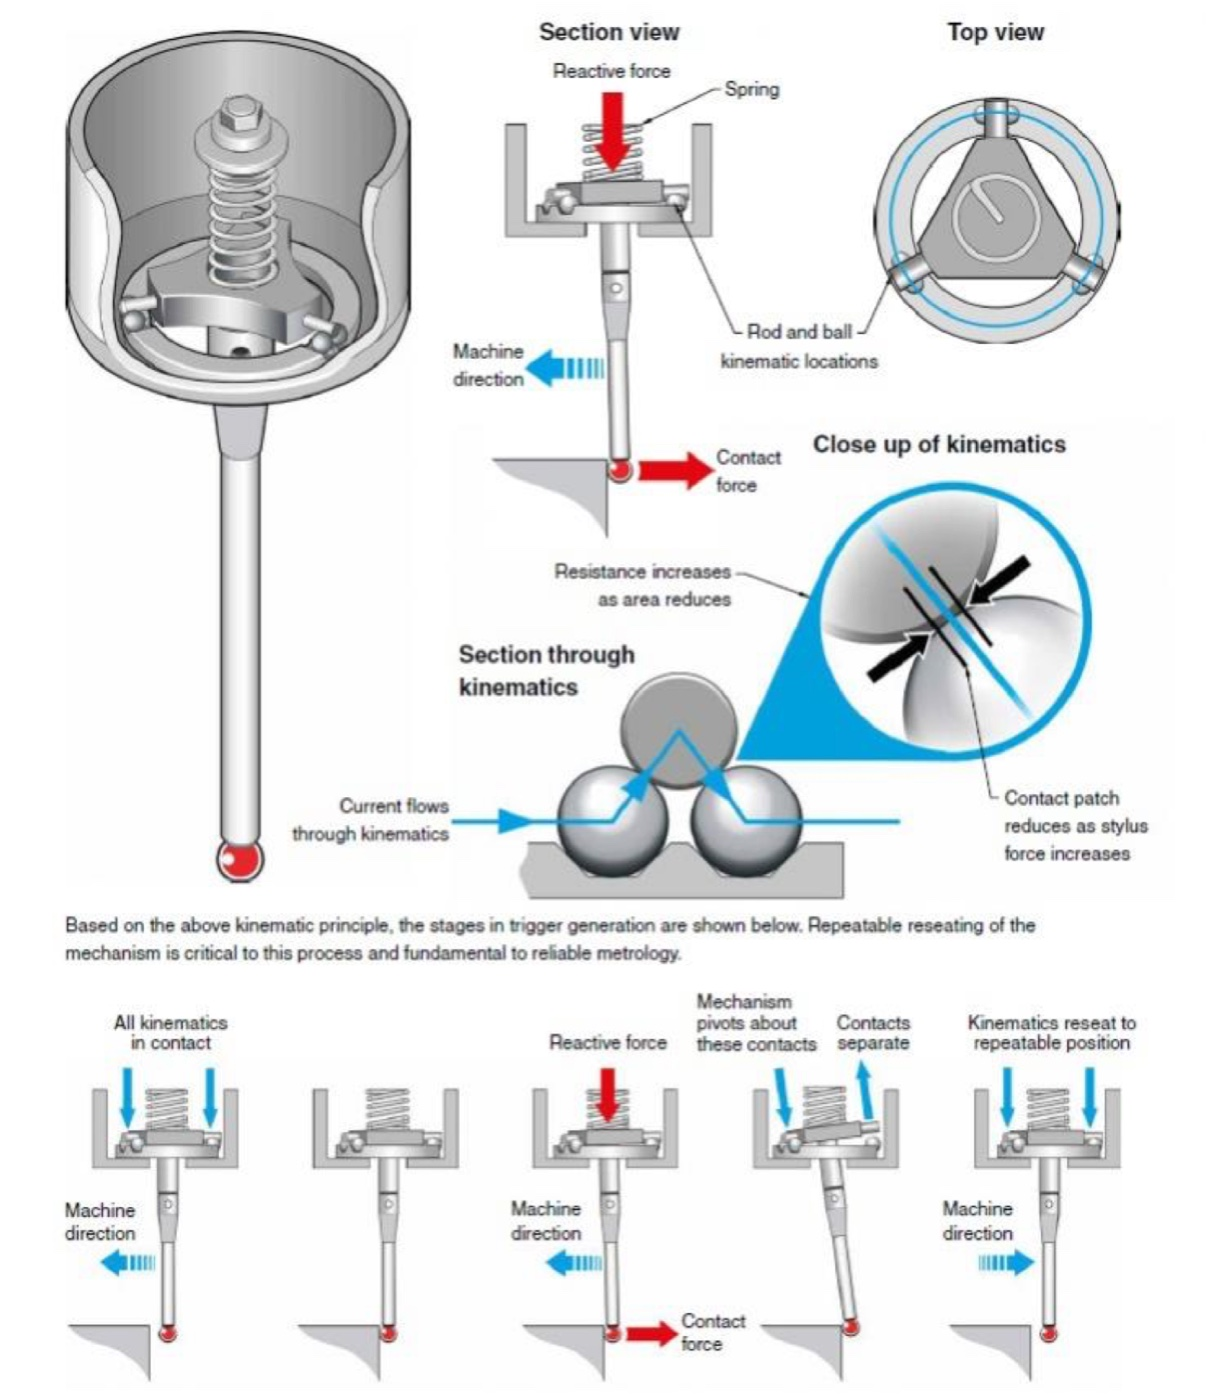
\includegraphics[width=\linewidth,height=4.58333in,keepaspectratio]{images/touch-probe.jpg}
\end{center}

\subsection{}\label{section-3}

\subsection{\texorpdfstring{Tool reference
(\emph{presetting})}{Tool reference (presetting)}}\label{tool-reference-presetting}

Tool geometry can be measured in machine (\textbf{exposed time}) or by a
\textbf{tool presetter} (\textbf{masked time}). The latter is preferred
because it is faster and more accurate, and it allows to measure the
tool geometry without having to mount it on the machine.

\begin{itemize}
\tightlist
\item
  On-board presetting uses a fixed stylus/switched contact point in
  known position reachable by the tool
\item
  Tool presetting systems have a dummy spindle mount, a camera and a
  shadow projector
\end{itemize}

\begin{center}
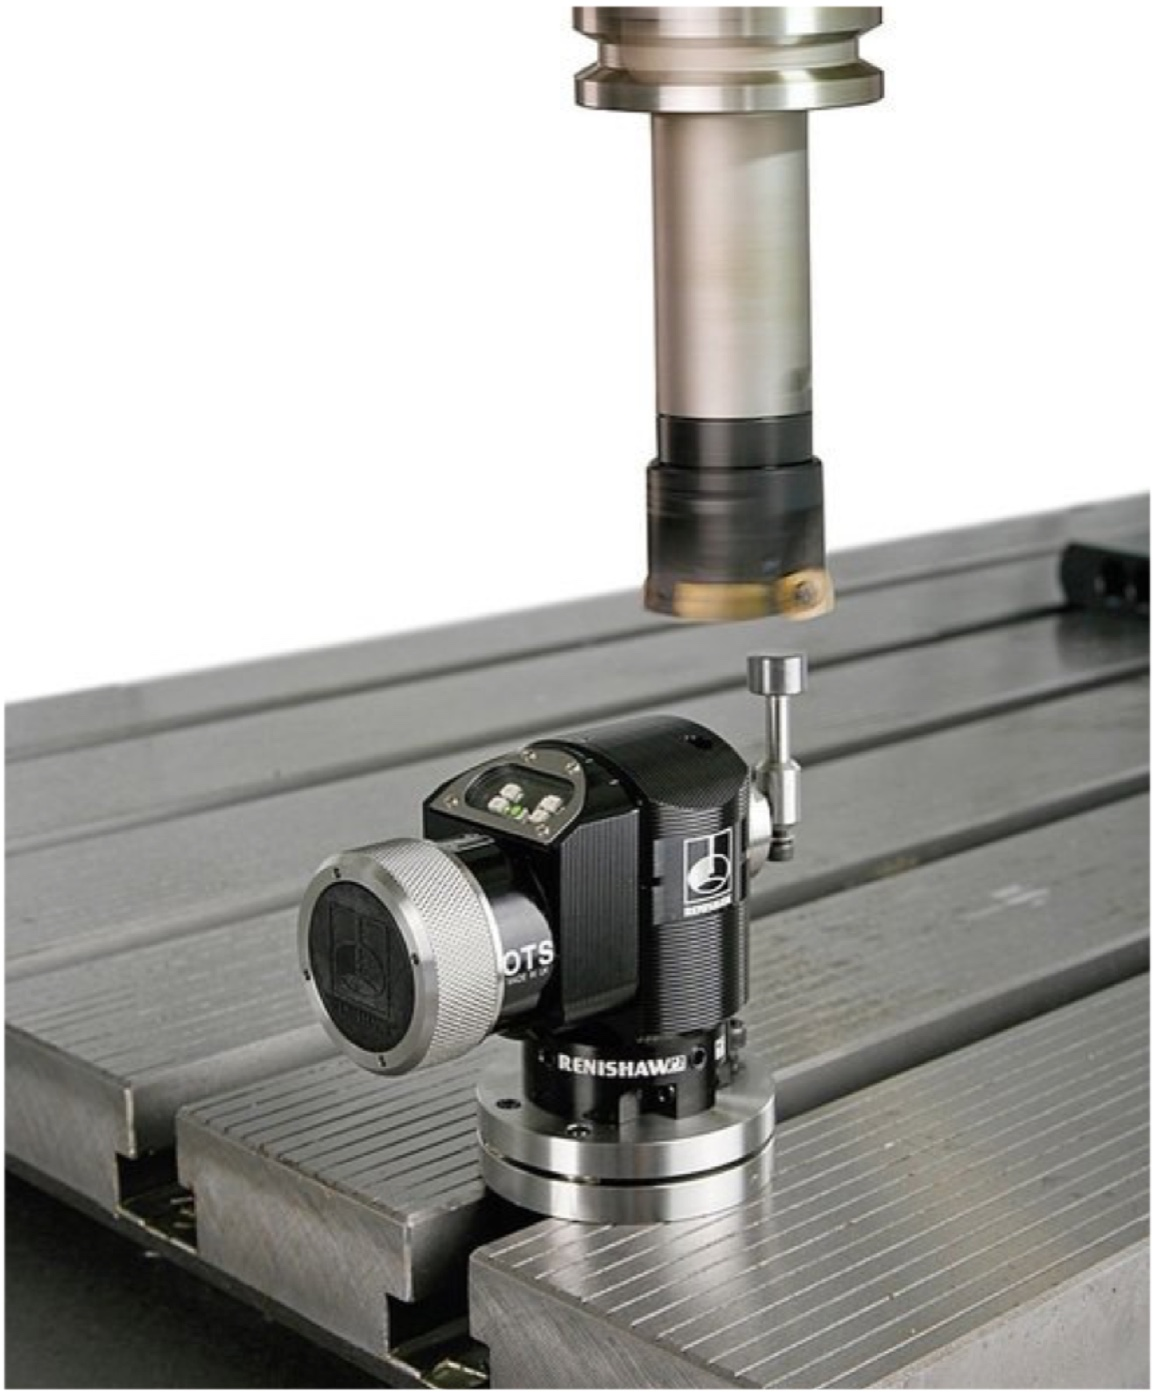
\includegraphics[width=\linewidth,height=2.60417in,keepaspectratio]{images/presetting-1.jpg}
\end{center}
\begin{center}
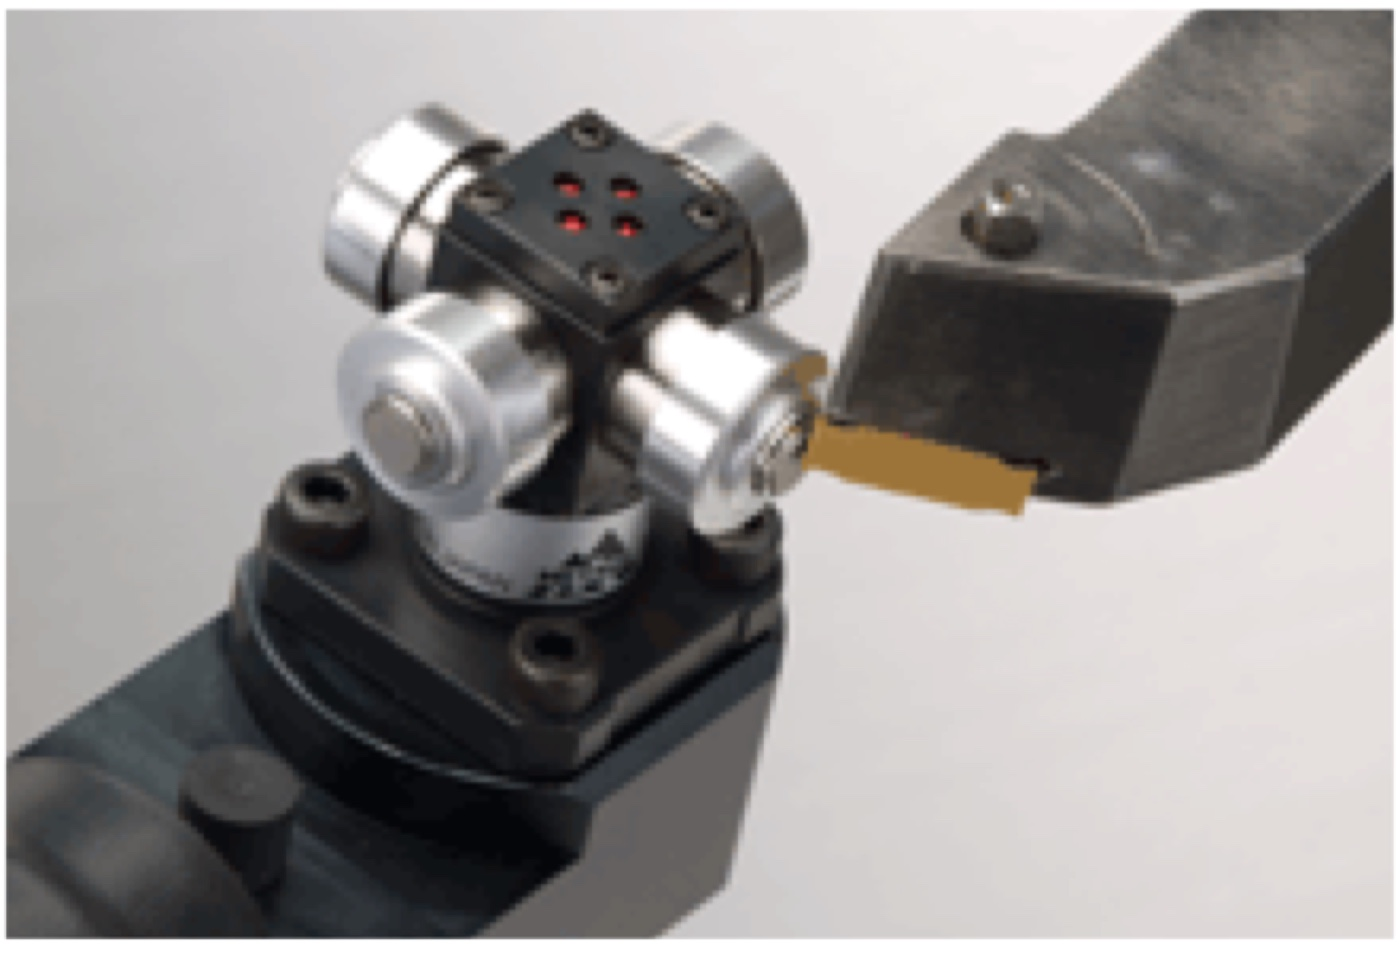
\includegraphics[width=\linewidth,height=2.60417in,keepaspectratio]{images/presetting-3.jpg}
\end{center}
\begin{center}
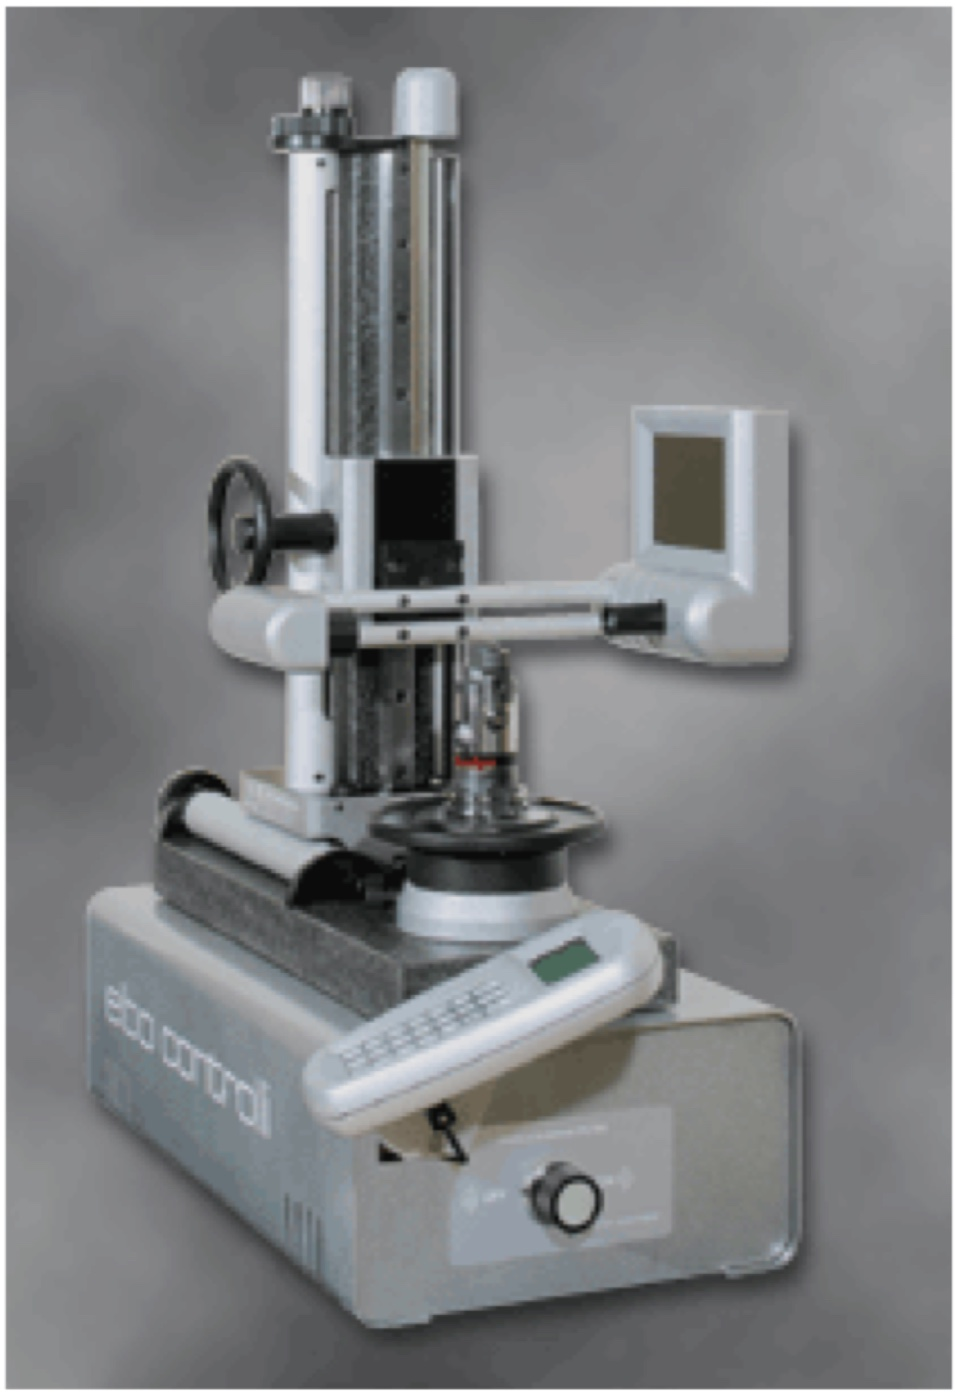
\includegraphics[width=\linewidth,height=2.60417in,keepaspectratio]{images/presetting-2.jpg}
\end{center}

\subsection{On-board presetting}\label{on-board-presetting}

\subsection{Tool presetter}\label{tool-presetter}

\subsection{Automation}\label{automation-1}

According to the Yardstick of Automation:

\begin{itemize}
\tightlist
\item
  most CNC machines are at Level A4
\item
  Level A5 requires post-machining automated inspection and feedback to
  the CNC controller and \textbf{to the part-program}
\end{itemize}

\begin{center}
\includegraphics[width=\linewidth,height=2.91667in,keepaspectratio]{1-machine_tools_files/mediabag/images-1/yardstick-loop.pdf}
\end{center}

\begin{itemize}
\tightlist
\item
  a validated \textbf{process model} can be required to implement A5,
  which is not necessarily available for most machining processes
\item
  empirical models (\emph{machine learning}) can be used to implement
  A5, but they require a lot of data and are not always reliable
\end{itemize}

\subsection{Machining cycle}\label{machining-cycle}

The general sequence for machining a part is:

\begin{center}
\includegraphics[width=\linewidth,height=2.70833in,keepaspectratio]{1-machine_tools_files/mediabag/images-1/machining-cycle.pdf}
\end{center}

The section within the red box is the \textbf{machining cycle}, i.e.~the
sequence of operations that can be cyclically repeated for each part

\subsection{Part-program structure}\label{part-program-structure}

The structure of a part program generally follows a common structure:

\begin{itemize}
\tightlist
\item
  \textbf{setups}
\item
  \textbf{roughing} section: removes the bulk of the material, usually
  with a large tool and high feedrate, leaving a small allowance for
  finishing
\item
  \textbf{finishing} section: removes the remaining material with a
  small tool and low feedrate (final geometry)
\item
  \textbf{reset} of the machine to a safe position and end of program
\end{itemize}

\begin{center}
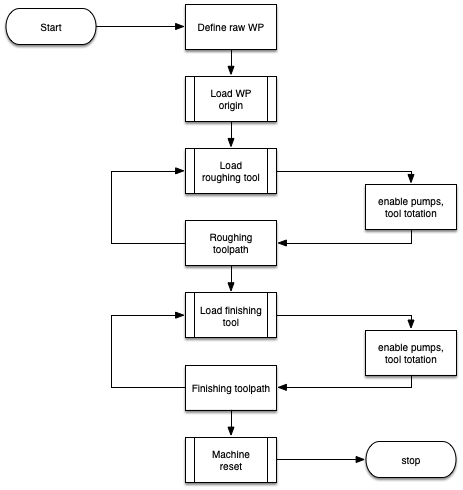
\includegraphics[width=\linewidth,height=5.10417in,keepaspectratio]{images-1/part-program.png}
\end{center}

\subsection{Toolpaths}\label{toolpaths}

\begin{center}
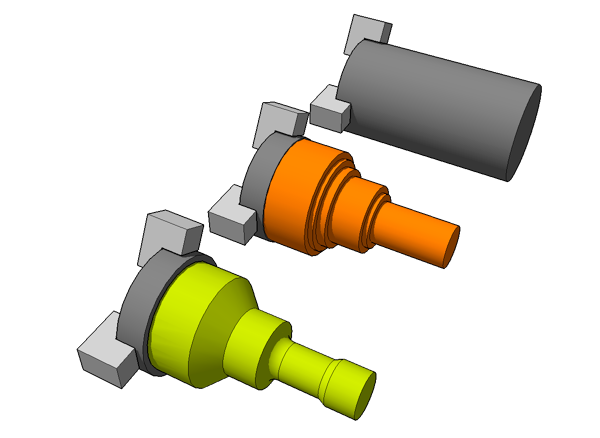
\includegraphics[width=\linewidth,height=5.10417in,keepaspectratio]{images-1/turning-process.png}
\end{center}

\begin{itemize}
\tightlist
\item
  Roughing and finishing may require different tools for different
  geometries
\item
  Roughing typically follows simple, stepped trajectories
\item
  Roughing allowance (excess material) is usually in the range of

  \begin{itemize}
  \tightlist
  \item
    0.5--1 mm for turning
  \item
    0.2--0.5 mm for milling
  \end{itemize}
\end{itemize}

\subsection{Workpiece Origin}\label{workpiece-origin}

In turning, X coordinates are in \textbf{diameters}. Two typical choices
for origin:

\begin{itemize}
\tightlist
\item
  rightmost axial point on finished workpiece
\item
  on the machine origin (fixtures must be taken into consideration)
\end{itemize}

Common choice for WP origin among machinists is the \textbf{rightmost
axial point on finished workpiece} (turning) and \textbf{topmost point
on the finished workpiece} (milling). This choice allows to quickly spot
in a program \textbf{safe} fast motions (positive \(z\)), from
\textbf{dangerous} fast motions (negative \(z\)) that can crash the tool
into the workpiece or fixture.

\subsection{G-Code}\label{g-code}

\textbf{ISO language} (ISO/DIN 6983): sequence of
\texttt{{[}C{]}{[}arg{]}} where \texttt{C} is a letter and \texttt{arg}
is a number. Valid commands are:

{\def\LTcaptype{none} % do not increment counter
\begin{longtable}[]{@{}ll@{}}
\toprule\noalign{}
Cod. & Command \\
\midrule\noalign{}
\endhead
\bottomrule\noalign{}
\endlastfoot
A & Rotation about X \\
B & Rotation about Y \\
C & Rotation about Z \\
D & Tool diameter compensation \\
E & Secondary feedrate \\
F & Feedrate \\
G & Preparatory function \\
H & --- \\
I & Circle center, X \\
\end{longtable}
}

{\def\LTcaptype{none} % do not increment counter
\begin{longtable}[]{@{}ll@{}}
\toprule\noalign{}
Cod. & Command \\
\midrule\noalign{}
\endhead
\bottomrule\noalign{}
\endlastfoot
J & Circle center, Y \\
K & Circle center, Z \\
L & --- \\
M & Machine function \\
N & Block number \\
O & --- \\
P & Third motion along X \\
Q & Third motion along Y \\
& \\
\end{longtable}
}

{\def\LTcaptype{none} % do not increment counter
\begin{longtable}[]{@{}ll@{}}
\toprule\noalign{}
Cod. & Command \\
\midrule\noalign{}
\endhead
\bottomrule\noalign{}
\endlastfoot
R & Third motion along Z \\
S & Spindle speed \\
T & Tool number \\
U & Second motion along X \\
V & Second motion along Y \\
W & Second motion along Z \\
X & Motion along X \\
Y & Motion along Y \\
Z & Motion along Z \\
\end{longtable}
}

\subsection{Punch tape}\label{punch-tape}

\begin{itemize}
\tightlist
\item
  \href{https://en.wikipedia.org/wiki/G-code}{G-Code} was developed
  during 1950s
\item
  Computers only had \textbf{punch tapes} as input devices
\item
  Language had to be concise
\end{itemize}

\begin{center}
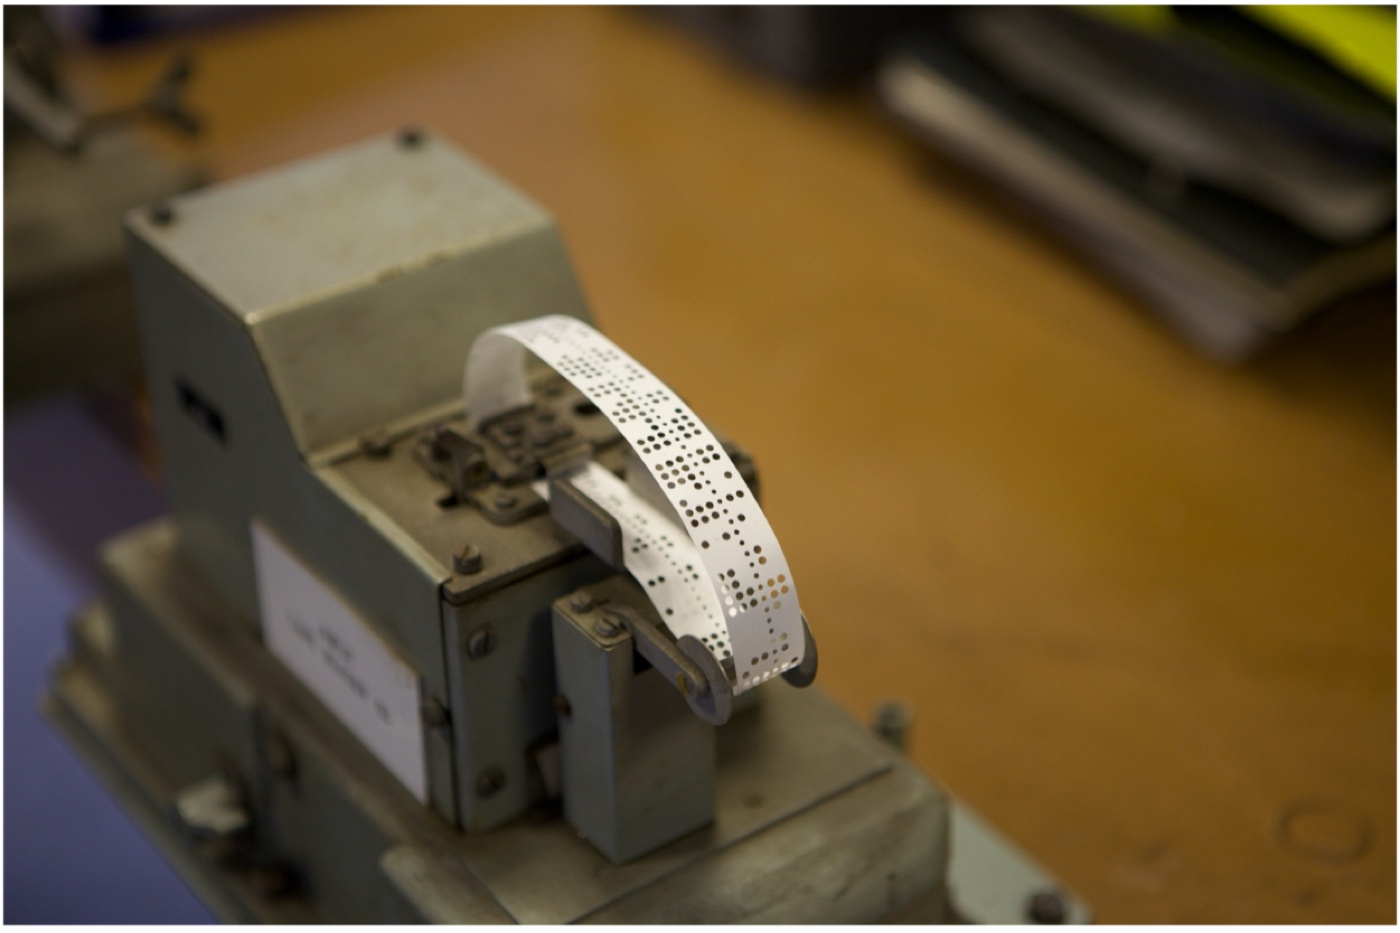
\includegraphics[width=\linewidth,height=2.91667in,keepaspectratio]{images/punch-tape-photo.jpg}
\end{center}

\begin{center}
\includegraphics[width=\linewidth,height=2.91667in,keepaspectratio]{1-machine_tools_files/mediabag/images-1/punch-tape.pdf}
\end{center}

\subsection{G-code functions}\label{g-code-functions}

Types of functions:

\begin{itemize}
\tightlist
\item
  Preparatory functions (\texttt{G}, \texttt{T})
\item
  Positioning functions (\texttt{X}, \texttt{Y}, \texttt{Z}, \texttt{A},
  \texttt{B}, \texttt{C})
\item
  Machine functions (\texttt{M})
\end{itemize}

\texttt{G} functions:

\begin{itemize}
\tightlist
\item
  \texttt{G00}: \textbf{rapid positioning}
\item
  \texttt{G01}: \textbf{linear interpolation}
\item
  \texttt{G02/G03}: \textbf{circular interpolation} (CW/CCW)
\end{itemize}

\begin{Shaded}
\begin{Highlighting}[]
\NormalTok{N1 T1 S500.0 M3                             ; tool n°1, CW rotation, 500 rpm}
\NormalTok{N2 M8;                                      ; fluid jets ON}
\NormalTok{N3 G00 X60.0 Z0.0;                          ; rapid positioning}
\NormalTok{N4 G01 X{-}0.5 Z0.0 F1000.0                   ; facing}
\NormalTok{N5 G01 X20.0 F1000.0}
\NormalTok{N6 G03 X40.0 Z{-}5.0 I30.0 K{-}10.0 F1000.0     ; arc R=10.0}
\NormalTok{...}
\NormalTok{N128 M30                                    ; fine programma}
\end{Highlighting}
\end{Shaded}

\subsection{Example: turning}\label{example-turning}

\begin{center}
\includegraphics[width=\linewidth,height=4.89583in,keepaspectratio]{1-machine_tools_files/mediabag/images-1/turning-part.pdf}
\end{center}

\subsection{Example: turning ---
roughing}\label{example-turning-roughing}

\begin{center}
\includegraphics[width=\linewidth,height=1.77083in,keepaspectratio]{1-machine_tools_files/mediabag/images-1/turning-rough.pdf}
\end{center}

\begin{Shaded}
\begin{Highlighting}[]
\NormalTok{N10 G00 X61.0 Z7.0}
\NormalTok{N11 G01 Z{-}94.5 F1000.0}
\NormalTok{N12 G01 G91 X5.0 F2000.0}
\NormalTok{N13 G00 Z7.0}
\NormalTok{N14 G00 X51.0}
\NormalTok{N15 G01 Z{-}88 F1000.0}
\NormalTok{N16 G01 G91 X5.0 F2000.0}
\NormalTok{N17 G00 Z7.0}
\end{Highlighting}
\end{Shaded}

\begin{Shaded}
\begin{Highlighting}[]
\NormalTok{N18 G00 X41.0 Z7.0}
\NormalTok{N19 G01 Z{-}59.4 F1000.0}
\NormalTok{N20 G01 G91 X5.0 F2000.0}
\NormalTok{N21 G00 Z7.0}
\NormalTok{N22 G00 X32.0}
\NormalTok{N23 G01 Z{-}57.6 F1000.0}
\NormalTok{N24 G01 G91 X5.0 F2000.0}
\NormalTok{N25 G00 Z7.0}
\end{Highlighting}
\end{Shaded}

\subsection{Example: turning ---
finishing}\label{example-turning-finishing}

\begin{center}
\includegraphics[width=\linewidth,height=1.77083in,keepaspectratio]{1-machine_tools_files/mediabag/images-1/turning-finish.pdf}
\end{center}

\begin{Shaded}
\begin{Highlighting}[]
\NormalTok{N31 G00 X70.0 Z0.0}
\NormalTok{N32 G00 X35.0}
\NormalTok{N33 G01 X0.0 F1000.0 S2000.0}
\NormalTok{N34 G00 Z5.0}
\NormalTok{N35 G00 X30.0}
\NormalTok{N36 G01 Z{-}20.0}
\NormalTok{N37 G01 X25.0 Z{-}25}
\end{Highlighting}
\end{Shaded}

\begin{Shaded}
\begin{Highlighting}[]
\NormalTok{N38 G01 Z{-}52.0}
\NormalTok{N39 G02 X45.0 Z{-}62.0 I10.0 K0.0}
\NormalTok{N40 G01 Z{-}85.0}
\NormalTok{N41 G01 G91 X20.0 Z{-}15.0}
\NormalTok{N42 G01 G90 Z{-}150.0}
\NormalTok{N43 G00 X70.0}
\NormalTok{N44 G00 Z20.0}
\NormalTok{...}
\NormalTok{N98 M30}
\end{Highlighting}
\end{Shaded}

\subsection{Example: milling}\label{example-milling}

\begin{itemize}
\tightlist
\item
  WP origin is usually placed in \(y,y\) plane on a geometry feature
  where most of the dimensions are referenced to, e.g.~the bottom-left
  corner of a rectangular pocket
\item
  The \(z\) coordinate is set to the topmost surface on the
  \textbf{finished part}:

  \begin{itemize}
  \tightlist
  \item
    the very first roughing operation will remove the excess material
    and reach the finished surface, which will be used as reference for
    all subsequent operations
  \item
    any subsequent operation is carried out at a \textbf{negative \(z\)}
    coordinate, which is the depth of cut below the finished surface
  \end{itemize}
\end{itemize}

\begin{center}
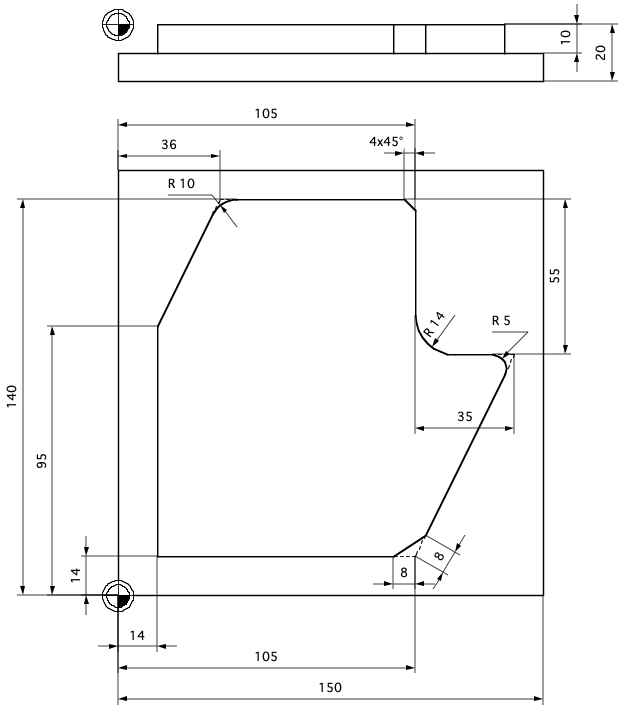
\includegraphics[width=\linewidth,height=5in,keepaspectratio]{images-1/milling-part.png}
\end{center}

\subsection{Example: milling}\label{example-milling-1}

\begin{codelisting}

\caption{\texttt{G-code language}}

\begin{Shaded}
\begin{Highlighting}[]
\NormalTok{\%es1 G71 *}
\NormalTok{N10 G30 G17 X+0 Y+0 Z{-}20*}
\NormalTok{N20 G31 X+150 Y+150 Z+0*}
\NormalTok{N30 G247 Q339=+1*}
\NormalTok{N40 T1 G17 S5000 F4000*}
\NormalTok{N50 G00 G90 X+14 Y{-}15 Z+10 G40 M8*}
\NormalTok{N60 G00 Z{-}10 G40*}
\NormalTok{N70 G01 Y+95 G41 F4000*}
\NormalTok{N80 G01 X+36 Y+140*}
\NormalTok{N90 G25 R10*}
\NormalTok{N100 G01 X+105*}
\NormalTok{N110 G24 R4*}
\NormalTok{N120 G01 G91 Y{-}55*}
\NormalTok{N130 G25 R14*}
\NormalTok{N140 G01 G91 X+35*}
\NormalTok{N150 G25 R5*}
\NormalTok{N160 G01 G90 X+105 Y+14*}
\NormalTok{N170 G24 R8*}
\NormalTok{N180 G01 X{-}15*}
\NormalTok{N190 G00 Z+10 G40*}
\NormalTok{N200 G38 M30*}
\NormalTok{N99999999 \%es1 G71 *}
\end{Highlighting}
\end{Shaded}

\end{codelisting}

\begin{figure}[H]

{\centering \pandocbounded{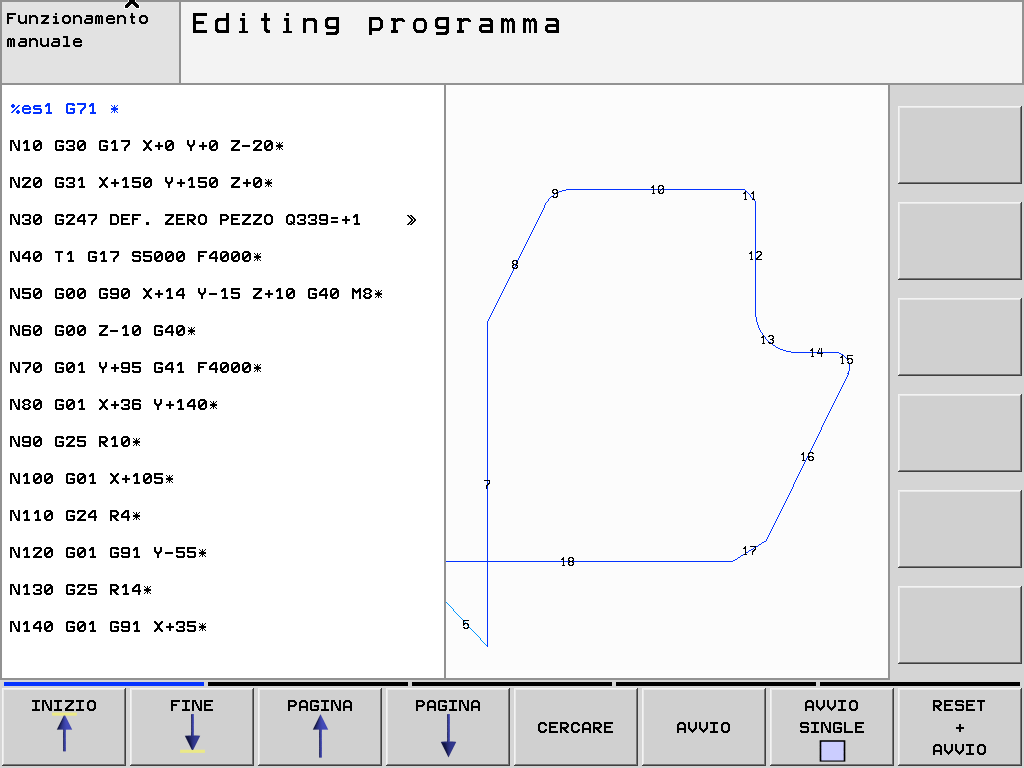
\includegraphics[keepaspectratio]{images-1/heidenhain-1.png}}

}

\caption{Heidenhain CNC - interactive programming}

\end{figure}%

\subsection{Program check}\label{program-check}

\begin{codelisting}

\caption{\texttt{G-code language}}

\begin{Shaded}
\begin{Highlighting}[]
\NormalTok{\%es1 G71 *}
\NormalTok{N10 G30 G17 X+0 Y+0 Z{-}20*}
\NormalTok{N20 G31 X+150 Y+150 Z+0*}
\NormalTok{N30 G247 Q339=+1*}
\NormalTok{N40 T1 G17 S5000 F4000*}
\NormalTok{N50 G00 G90 X+14 Y{-}15 Z+10 G40 M8*}
\NormalTok{N60 G00 Z{-}10 G40*}
\NormalTok{N70 G01 Y+95 G41 F4000*}
\NormalTok{N80 G01 X+36 Y+140*}
\NormalTok{N90 G25 R10*}
\NormalTok{N100 G01 X+105*}
\NormalTok{N110 G24 R4*}
\NormalTok{N120 G01 G91 Y{-}55*}
\NormalTok{N130 G25 R14*}
\NormalTok{N140 G01 G91 X+35*}
\NormalTok{N150 G25 R5*}
\NormalTok{N160 G01 G90 X+105 Y+14*}
\NormalTok{N170 G24 R8*}
\NormalTok{N180 G01 X{-}15*}
\NormalTok{N190 G00 Z+10 G40*}
\NormalTok{N200 G38 M30*}
\NormalTok{N99999999 \%es1 G71 *}
\end{Highlighting}
\end{Shaded}

\end{codelisting}

\begin{figure}[H]

{\centering \pandocbounded{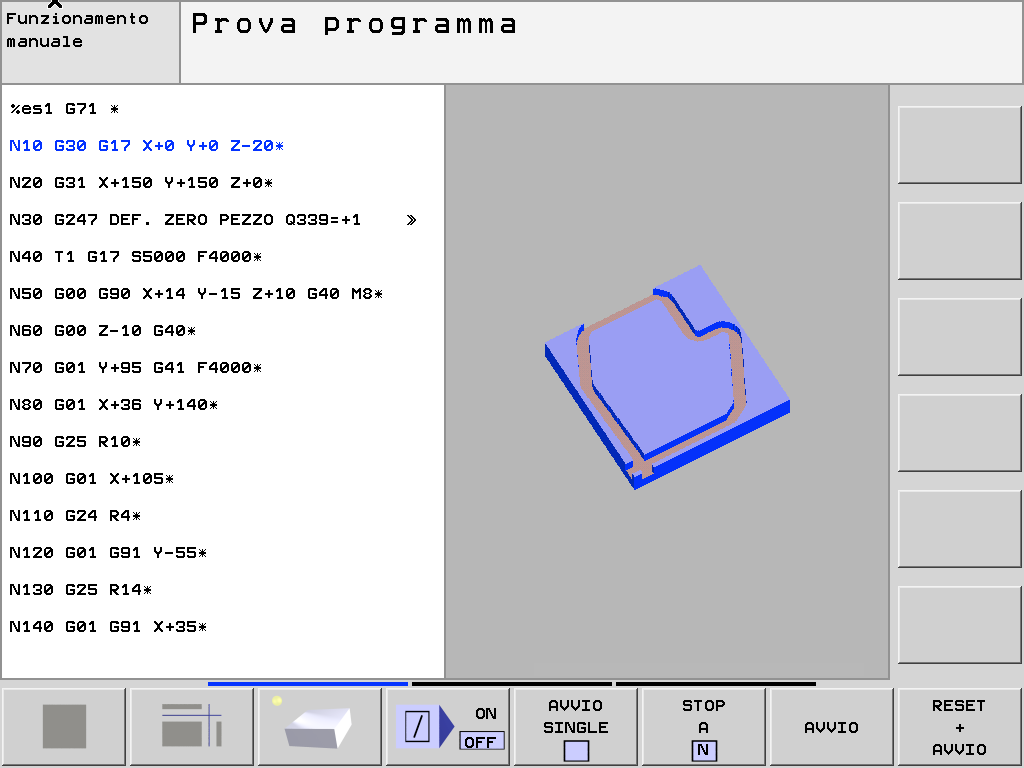
\includegraphics[keepaspectratio]{images-1/heidenhain-2.png}}

}

\caption{Heidenhain CNC - program preview}

\end{figure}%

\subsection{Advanced languages}\label{advanced-languages}

Different CNC manufacturers implement proprietary languages that extend
the basic G-code with advanced features:

\begin{itemize}
\tightlist
\item
  Explicit, richer syntax
\item
  Conversational/interactive programming (\emph{zero-handbook})
\item
  Macros
\item
  Parametric programming
\end{itemize}

\begin{codelisting}

\caption{\texttt{Heidenhain language}}

\begin{Shaded}
\begin{Highlighting}[]
\NormalTok{0  BEGIN PGM es1 MM}
\NormalTok{1  BLK FORM 0.1 Z  X+0  Y+0  Z{-}20}
\NormalTok{2  BLK FORM 0.2  X+150  Y+150  Z+0}
\NormalTok{3  CYCL DEF 247 DEF. ZERO PEZZO \textasciitilde{}}
\NormalTok{    Q339=+1    ;NUMERO ORIGINE}
\NormalTok{4  TOOL CALL 1 Z S5000 F4000}
\NormalTok{5  M8}
\NormalTok{6  L  X+10  Y{-}10  Z+10 R0 FMAX}
\NormalTok{7  L  Z{-}10 R0 FMAX}
\NormalTok{8  L  Y+95 RL F AUTO}
\NormalTok{9  L  X+36  Y+140}
\NormalTok{10 RND R10 F AUTO}
\NormalTok{11 L  X+105}
\NormalTok{12 CHF 4}
\NormalTok{13 L IY{-}55}
\NormalTok{14 RND R14}
\NormalTok{15 L IX+35}
\NormalTok{16 RND R5}
\NormalTok{17 L  X+105  Y+14}
\NormalTok{18 CHF 8}
\NormalTok{19 L  X{-}15}
\NormalTok{20 L  Z+10 R0 FMAX}
\NormalTok{21 STOP M30}
\NormalTok{22 END PGM es1 MM}
\end{Highlighting}
\end{Shaded}

\end{codelisting}

\section{CNC}\label{cnc}

\emph{Algorithms for Computer Numerical Control --- machining complex
shapes}

\begin{center}
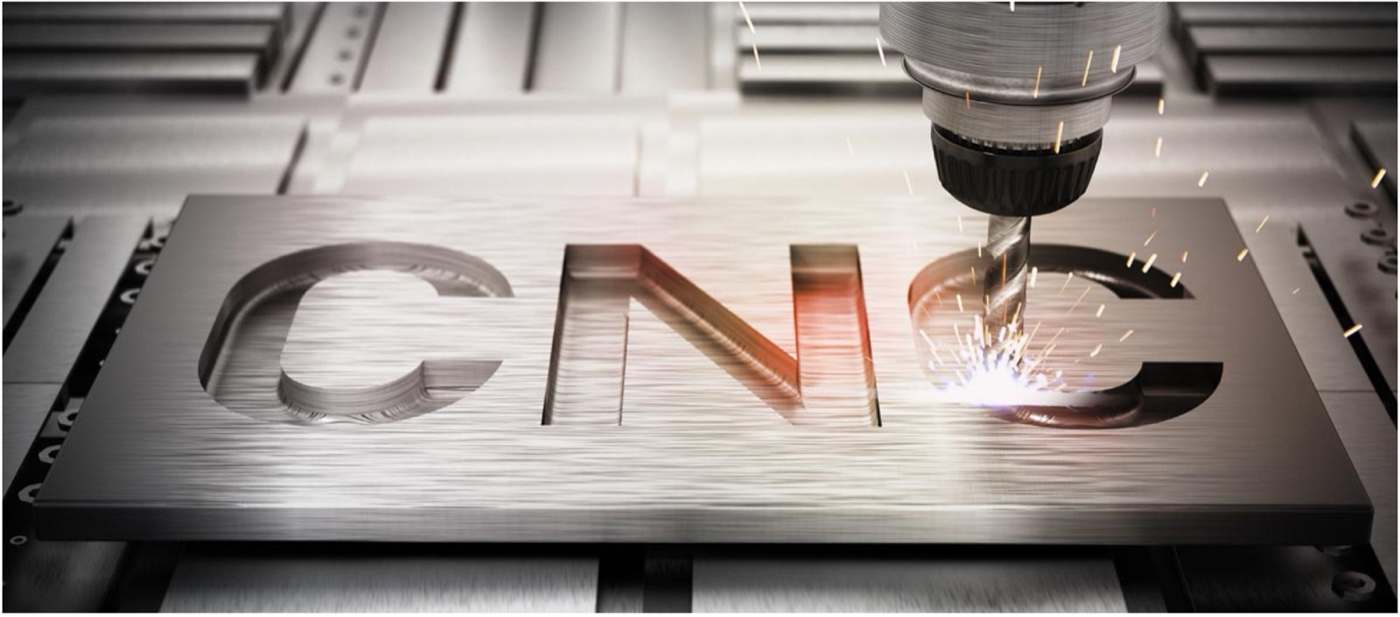
\includegraphics[width=\linewidth,height=3.125in,keepaspectratio]{images/cnc-photo.jpg}
\end{center}

\subsection{CNC kernel tasks}\label{cnc-kernel-tasks}

The \textbf{CNC kernel} is the part of the CNC controller that
implements the \textbf{real-time control loop}. It is responsible for:

\begin{itemize}
\tightlist
\item
  Understanding a part-program (parsing)
\item
  Generate velocity profiles (profiling)
\item
  Position interpolation (project trajectory on the machine axes)
\item
  Generate command signals (actuation) to the axes drives
\end{itemize}

\begin{tcolorbox}[enhanced jigsaw, arc=.35mm, bottomrule=.15mm, bottomtitle=1mm, breakable, colback=white, colbacktitle=quarto-callout-note-color!10!white, colframe=quarto-callout-note-color-frame, coltitle=black, left=2mm, leftrule=.75mm, opacityback=0, opacitybacktitle=0.6, rightrule=.15mm, title=\textcolor{quarto-callout-note-color}{\faInfo}\hspace{0.5em}{Note}, titlerule=0mm, toprule=.15mm, toptitle=1mm]

Beside these tasks, the rest of the CNC also takes care of the GUI,
programs selection, editing and storing, networking, tables management
(presets and tools), interaction with the PLC, and other non-real-time
tasks. The CNC kernel is the part of the CNC that is \textbf{real-time}
and must be implemented in a \textbf{real-time operating system} (RTOS)

\end{tcolorbox}

\subsection{Profiling}\label{profiling}

Profiling is where motion algorithms are implemented. For every block:

\begin{itemize}
\tightlist
\item
  preserve block length:
  \(\displaystyle\int_{t_a}^{t_b} f(\tau)\,\mathrm{d}\tau = l\)
\item
  limit acceleration to the maximum allowed by the machine
\item
  limit jerks, to minimize vibrations and mechanical stress
\end{itemize}

\subsection{Profiling}\label{profiling-1}

Discrete time-base (clock steps of \(t_q\)) and feedrate quantization.
Block durations must be scaled to a multiple of \(t_q\) yet maintaining
the same block length. The actual feedrate is reduced accordingly.

\[
\Delta t_1 = \frac{f_m - f_s}{a}, \quad
\Delta t_2 = \frac{f_m - f_e}{d}, \quad
\Delta t_m = \frac{l}{f_m} - \Delta t_1 \frac{f_m + f_s}{2 f_m} - \Delta t_2 \frac{f_e + f_m}{2 f_m}
\]

\[
\Delta t^* = \mathrm{int}\left(\frac{\Delta t}{t_q} + 1\right) t_q = \Delta t_1 + \Delta t_m^* + \Delta t_2, \qquad
\Delta t_m^* = \Delta t_m + \Delta t^* - \Delta t
\]

\subsection{Profiling}\label{profiling-2}

Discrete time-base (clock steps of \(t_q\)) and feedrate quantization.
Block durations must be scaled to a multiple of \(t_q\) yet maintaining
the same block length. The actual feedrate is reduced accordingly.

\[
\int_{t_s}^{t_e} f(\tau)\,\mathrm{d}\tau = \frac{\Delta t_1}{2}(f_m^* + f_s) + \Delta t_m^* f_m^* + \frac{\Delta t_2}{2}(f_m^* + f_e) = l
\]

\[
f_m^* = \frac{2l - f_s \Delta t_1 - f_e \Delta t_2}{\Delta t_1 + \Delta t_2 + 2\Delta t_m^*}, \qquad
a^* = \frac{f_m^* - f_s}{\Delta t_1}, \qquad
d^* = \frac{f_e - f_m^*}{\Delta t_2}
\]

\subsection{Profiling}\label{profiling-3}

In \textbf{short segments} there's no time enough to reach the nominal
feedrate: \(\Delta t_m \le 0\)

\[
\int_{t_s}^{t_e} f(\tau)\,\mathrm{d}\tau = \frac{a\Delta t_1^2 + d\Delta t_2^2}{2}; \quad a\Delta t_1 = d\Delta t_2
\]

\[
\frac{\Delta t_1^2 (a + a^2/d)}{2} = l
\]

\[
\begin{aligned}
\Delta t_1 &= \sqrt{\frac{2l}{a + a^2/d}} \\
\Delta t_2 &= \frac{a}{d}\Delta t_1 \\
\Delta t_2^* &= \Delta t^* - \Delta t_1
\end{aligned}
\qquad
f_m^*(\Delta t_1 + \Delta t_2^*) = 2l
\qquad
\begin{aligned}
a^* &= \frac{f_m^* - f_s}{\Delta t_1} \\
d^* &= \frac{f_e - f_m^*}{\Delta t_2^*}
\end{aligned}
\]

\subsection{Motion interpolation}\label{motion-interpolation}

\begin{itemize}
\tightlist
\item
  The speed profile is evaluated and integrated at each time tick:
  \(\lambda(t) = 1/L\int_0^t f(\tau)\,d\tau\)
\item
  The axes set-points are calculated with the parametric equation of the
  path
\item
  For a \textbf{linear motion}:
\end{itemize}

\[
\begin{aligned}
X(t) &= X_0 + \Delta X \lambda(t) \\
Y(t) &= Y_0 + \Delta Y \lambda(t) \\
Z(t) &= Z_0 + \Delta Z \lambda(t)
\end{aligned}
\]

\subsection{Motion interpolation}\label{motion-interpolation-1}

For \textbf{arc interpolation}:

\[
\begin{aligned}
X(t) &= X_c + R\cos(\vartheta_0 + \Delta\vartheta \lambda(t)) \\
Y(t) &= Y_c + R\sin(\vartheta_0 + \Delta\vartheta \lambda(t)) \\
Z(t) &= Z_0 + \Delta Z \lambda(t)
\end{aligned}
\]

Warning: feedrate may be reduced

\[
f_{m,a} = \min\left(f_m, \sqrt{aR}\right)
\]

\begin{center}
\includegraphics[width=\linewidth,height=3.4375in,keepaspectratio]{1-machine_tools_files/mediabag/images-1/arc-diagram.pdf}
\end{center}

\subsection{Motion interpolation}\label{motion-interpolation-2}

Two alternative G-code syntax for arcs:

\begin{itemize}
\tightlist
\item
  arch center:
  \texttt{G{[}02\textbar{}03{]}\ X{[}}\(X_f\)\texttt{{]}\ Y{[}}\(Y_f\)\texttt{{]}\ I{[}}\(I\)\texttt{{]}\ J{[}}\(J\)\texttt{{]}}
\item
  radius:
  \texttt{G{[}02\textbar{}03{]}\ X{[}}\(X_f\)\texttt{{]}\ Y{[}}\(Y_f\)\texttt{{]}\ R{[}}\(\pm R\)\texttt{{]}}
  (radius sign discriminates which arc to take)
\end{itemize}

\begin{center}
\includegraphics[width=\linewidth,height=2.91667in,keepaspectratio]{1-machine_tools_files/mediabag/images-1/arc-syntax.pdf}
\end{center}

\[
\begin{aligned}
\vartheta_0 &= \cos^{-1} I/R \\
\vartheta_f &= \cos^{-1} (X_f - X_c)/R \\
X_c &= X_0 + I \\
Y_c &= Y_0 + J \\
R &= \sqrt{I^2 + J^2} \\
R^2 &= (X_f - X_c)^2 + (Y_f - Y_c)^2
\end{aligned}
\]

\subsection{Motion interpolation}\label{motion-interpolation-3}

\textbf{Center coordinates} (two alternatives depending on the sign of
\(R\))

\[
\Delta x = X_f - X_0, \qquad \Delta y = Y_f - Y_0
\]

\[
X_c = X_0 + \frac{1}{2}\left(\Delta x - \mathrm{sign}(R)\,\frac{\sqrt{-\Delta y^2 (\Delta x^2 + \Delta y^2)(-4R^2 + \Delta x^2 + \Delta y^2)}}{\Delta x^2 + \Delta y^2}\right)
\]

\[
Y_c = Y_0 + \frac{\Delta y}{2} + \mathrm{sign}(R)\,\frac{\Delta x \sqrt{-\Delta y^2 (\Delta x^2 + \Delta y^2)(-4R^2 + \Delta x^2 + \Delta y^2)}}{2\Delta x^2 \Delta y + 2\Delta y^3}
\]

\subsection{Jerk}\label{jerk}

Jerk-limited profiling:

\begin{itemize}
\tightlist
\item
  corners in feedrate imply discontinuous acceleration
\item
  discontinuous acceleration mean \textbf{infinite jerk}
\item
  infinite jerk produces vibrations and mechanical stress
\item
  for \textbf{limited jerk profiling} each segment is split into 7
  ranges (vs.~3)
\end{itemize}

\subsection{Look-ahead feedrate
profile}\label{look-ahead-feedrate-profile}

The above presented algorithm assumes that the instant speed goes to
zero at each corner. This is not acceptable in real CNC machines, for
two reasons:

\begin{itemize}
\tightlist
\item
  \textbf{Problem 1:} tangent or semi-tangent blocks would result in
  excessive reduction of feedrate wrt nominal
\item
  \textbf{Problem 2:} it shall be possible to accelerate to nominal
  feedrate with continuous acceleration over \(n\) short segments, and
  it may take more than one segment to decelerate down to stop
\end{itemize}

To solve these issue we need to plan the velocity profile \textbf{across
multiple blocks} of G-Code. This is called \textbf{look-ahead}

\subsection{Look-ahead feedrate
profile}\label{look-ahead-feedrate-profile-1}

Approach:

\begin{enumerate}
\def\labelenumi{\arabic{enumi}.}
\tightlist
\item
  Calculate \(v_i\), \(v_m\), \(v_f\) for each block, considering
  \(v = v(s)\)
\item
  Forward step: from block 1 to block \(n\), calculate accelerations
  only
\item
  Backward step: from block \(n\) to block 1, calculate decelerations
  only and compose with accelerations
\item
  Change variable \(s \to t\) and get \(v = v(t)\)
\item
  Reshape \(v^* = \dfrac{v(t)}{k}\), where \(k = t_f / t_f^*\) and
  \(t_f^*\) is the multiple of \(t_q\) immediately larger than the total
  time \(t_f\) (block by block)
\end{enumerate}

\subsection{Constant Acc/Dec}\label{constant-accdec}

\begin{itemize}
\tightlist
\item
  We cannot calculate feed profiles in time abscissa, for we don't know
  the duration of each step
\item
  Thus we start planning in \textbf{curvilinear abscissa} \(s\):

  \begin{itemize}
  \tightlist
  \item
    \(s(t) = s_0 + v_0 t + a t^2/2\), and thus
    \(t(s) = \dfrac{1}{a}\left(-v_0 \pm \sqrt{2a(s - s_0) + v_0^2}\right)\)
  \item
    Since \(v(t(s)) = v_0 + a\, t(s)\), it follows that
    \(v(s) = \sqrt{2a(s - s_0) + v_0^2}\)
  \item
    So accelerations and decelerations follow a square root law of \(s\)
  \end{itemize}
\item
  In jerk-limited approach, we'd have a cubic root branch at the
  beginning and at the end of each acc/dec branch
\end{itemize}

\subsection{Look-ahead feedrate}\label{look-ahead-feedrate}

Step 1: calculate velocities:

\begin{itemize}
\tightlist
\item
  \(v_{i,i} = v_{f,i-1}\), or 0 for first sg.
\item
  \(v_{m,i} = f_i\) for G01
\item
  \(v_m = \min(f_i, \sqrt{aR})\) for G02/G03
\item
  \(v_{f,i} = \dfrac{v_{m,i} + v_{m,i+1}}{2}\cos\alpha_i\)
\item
  \(v_{f,i} = 0\) for last segment or if \(v_{m,i} = 0\)
\end{itemize}

\subsection{Forward step:
accelerations}\label{forward-step-accelerations}

Long segments, \(v_i < v_m\):

A. \(v_f > v_m\), \(s_0 < s_1 < s_2 < s_f\)

B. \(v_f < v_m\), \(s_0 < s_1 < s_f < s_2\)

\subsection{Forward step:
accelerations}\label{forward-step-accelerations-1}

Long segments, \(v_i > v_m\):

A. \(v_f > v_m\), \(s_1 < s_0 < s_2 < s_f\)

B. \(v_f < v_m\), \(s_1 < s_0 < s_f < s_2\)

\subsection{Forward step:
accelerations}\label{forward-step-accelerations-2}

Short segments:

\begin{itemize}
\tightlist
\item
  \(s_0 < s_f < s_1\)
\item
  \(v_f\) and \(s_2\) are not relevant
\end{itemize}

\subsection{Forward step:
accelerations}\label{forward-step-accelerations-3}

Short segments:

\begin{itemize}
\tightlist
\item
  If \(v_i\) is large enough, fallback to long segment cases
\end{itemize}

\subsection{Backward step:
decelerations}\label{backward-step-decelerations}

\begin{itemize}
\tightlist
\item
  Same approach as forward step
\item
  For each block, select the path going from \((s_0, v_i)\) to
  \((s_f, v_f)\)
\end{itemize}

\subsection{9 Possible cases}\label{possible-cases}

\subsection{Change of variable}\label{change-of-variable}

\subsubsection{Back to time abscissa}\label{back-to-time-abscissa}

Convert back \textbf{from curvilinear abscissa to time}, one block at a
time:

\begin{itemize}
\tightlist
\item
  Calculate \(v(t) = v_0 + at\), \(s(t) = s_0 + v_0 t + at^2/2\) in the
  ranges \([s_i, s_1]\), \([s_1, s_2]\), \([s_2, s_f]\)
\item
  Calculate timings \(t_1\), \(t_2\), \(t_f\)
\end{itemize}

\subsubsection{Reshape for discrete
time}\label{reshape-for-discrete-time}

\begin{itemize}
\tightlist
\item
  Calculate \(t_f^* = \lceil t_f / t_q + 1 \rceil t_q\)
\item
  Calculate \(k = t_f^* / t_f\)
\item
  \textbf{Rescale feedrate} so that \(v^*(t) = \dfrac{v(t)}{k}\)
\end{itemize}

\subsection{Receding horizon}\label{receding-horizon}

\begin{itemize}
\tightlist
\item
  This algorithm requires a sequence of blocks starting and ending at
  zero feedrate
\item
  You can assume that \texttt{G00} blocks mark full stops at corners
\item
  Nonetheless, a program can consist in thousands of sequential
  G01/G02/G03 blocks: memory problem
\item
  \textbf{Solution:}

  \begin{itemize}
  \tightlist
  \item
    At run time, pre-elaborate a buffer made of a limited number of
    blocks (say 100) assuming the last one stops (look-ahead buffer)
  \item
    Re-calculate the moving buffer as soon as a block is done by adding
    a new block at the end (FIFO): start backward (dec) until no change,
    then forward (acc)
  \item
    The buffer size depends on available memory and on computation time
    (must be shorter than the time needed to execute the buffer);
    calculations are done in parallel in a separate thread
  \end{itemize}
\end{itemize}

\section{Errors in machine tools}\label{errors-in-machine-tools}

\emph{Machine tools are precision systems --- laser interferometry}

\begin{center}
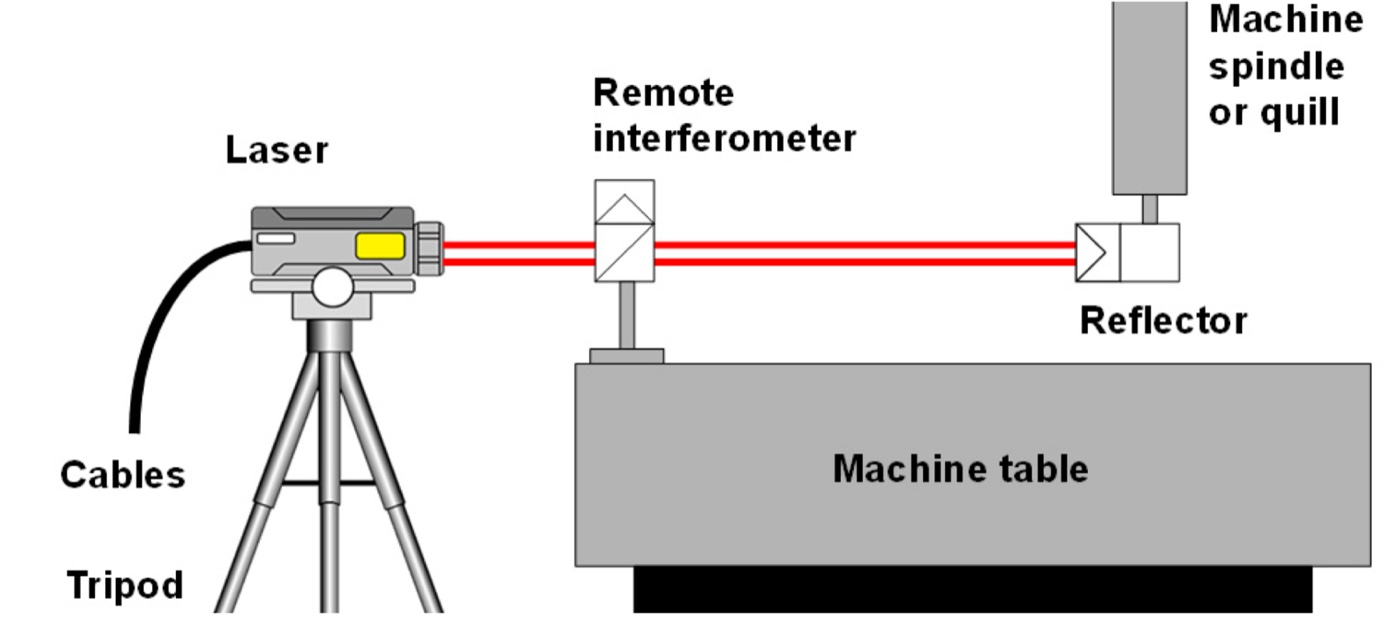
\includegraphics[width=\linewidth,height=3.125in,keepaspectratio]{images/laser-interferometry.jpg}
\end{center}

\subsection{Machining error sources}\label{machining-error-sources}

\begin{itemize}
\tightlist
\item
  {Process error sources}: tool/workpiece interaction (minimized by
  proper process conditions)
\item
  \textbf{Structural error sources}: time-dependent, eventually become
  stable and can be compensated
\item
  {Machine error sources}: more difficult to compensate, potentially
  ever changing
\end{itemize}

\subsection{Error Compensation (A5)}\label{error-compensation-a5}

Compensating for error means to \textbf{measure errors} and to
\textbf{apply corrections} to the machine tool commands. This is a
\textbf{closed-loop control} approach

\begin{itemize}
\tightlist
\item
  Adaptive control systems (A/C) = \textbf{evaluation} attribute (A5)
\item
  Factors under evaluation:

  \begin{itemize}
  \tightlist
  \item
    forces/deflections
  \item
    machining errors
  \item
    \textbf{thermoelastic} dilatations/deformations
  \end{itemize}
\end{itemize}

\subsection{Profiling errors}\label{profiling-errors}

Look-ahead can alter trajectory, especially at corners:

\begin{itemize}
\tightlist
\item
  More evident at high speed
\item
  When a sharp corner is needed, use curls or disable look-ahead
\end{itemize}

\pandocbounded{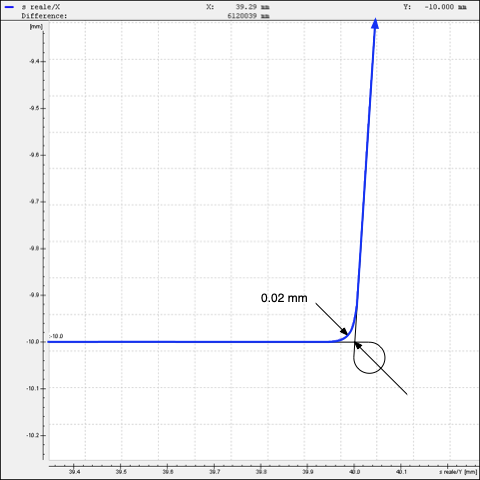
\includegraphics[keepaspectratio]{images-1/corner.png}}

\subsection{Feedrate-related errors}\label{feedrate-related-errors}

\begin{figure}[H]

{\centering \pandocbounded{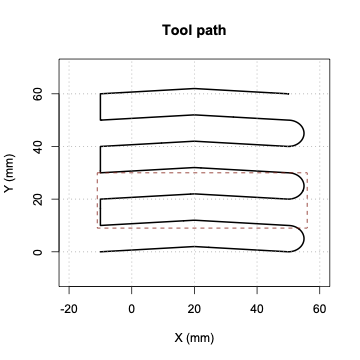
\includegraphics[keepaspectratio]{images-1/toolpath.png}}

}

\caption{Toolpath with sharp and shallow corners, long and short
segments}

\end{figure}%

\begin{figure}[H]

{\centering \pandocbounded{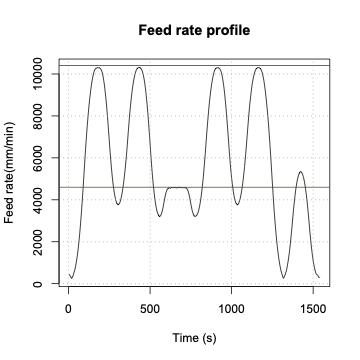
\includegraphics[keepaspectratio]{images-1/feed_rate.png}}

}

\caption{Feedrate profile: actual feedrate is rarely nominal}

\end{figure}%

\subsection{Positioning errors}\label{positioning-errors}

\begin{center}
\includegraphics[width=\linewidth,height=4.79167in,keepaspectratio]{1-machine_tools_files/mediabag/images-1/positioning-errors.pdf}
\end{center}

\subsection{Squareness errors}\label{squareness-errors}

\begin{center}
\includegraphics[width=\linewidth,height=4.79167in,keepaspectratio]{1-machine_tools_files/mediabag/images-1/squareness-errors.pdf}
\end{center}

\subsection{Elementary errors}\label{elementary-errors}

\begin{itemize}
\tightlist
\item
  Three linear errors per axis (linearity, straightness, undulation)
\item
  Three angular errors per axis (roll, pitch, yaw)
\item
  Two squareness errors between axes 1 and 2
\item
  Two squareness errors between axes 3 and 2
\item
  Total of 18 + 4 = 22 elementary errors, 18 of which are
  position-dependent
\end{itemize}

\subsection{Laser interferometer}\label{laser-interferometer}

\begin{center}
\includegraphics[width=\linewidth,height=4.89583in,keepaspectratio]{1-machine_tools_files/mediabag/images-1/interferometer-paths.pdf}
\end{center}

\subsection{Laser interferometer}\label{laser-interferometer-1}

\begin{figure}[H]

{\centering 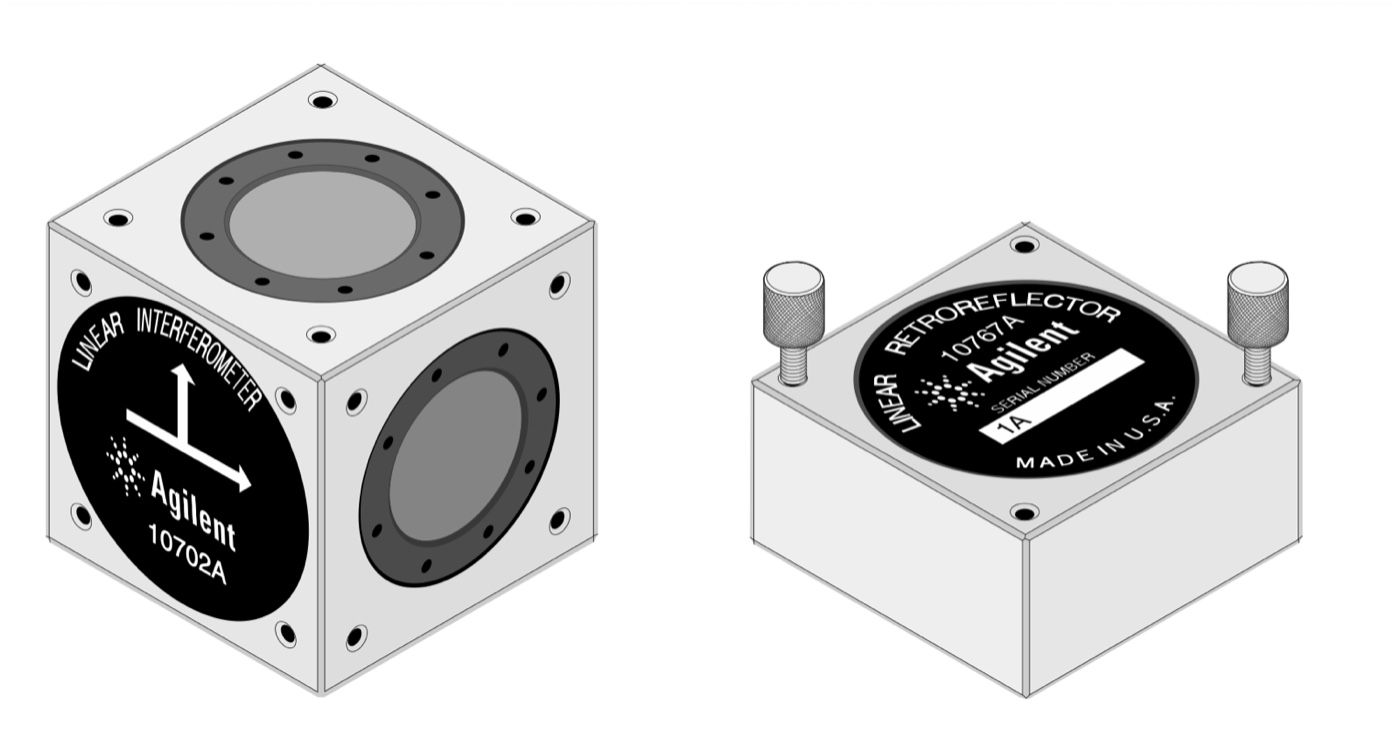
\includegraphics[width=\linewidth,height=4.89583in,keepaspectratio]{images/interferometer-optics.jpg}

}

\caption{Agilent beam splitter and retro-reflector}

\end{figure}%

\subsection{Linearity measurement}\label{linearity-measurement}

\begin{itemize}
\tightlist
\item
  This is the simplest measurement
\item
  The laser beam is reflected by a mirror mounted on the axis and the
  interferometer measures the distance travelled by the axis
\item
  It is a way to \textbf{calibrate} and to verify the
  \textbf{positioning accuracy} of the axis encoder
\end{itemize}

\begin{figure}[H]

{\centering \pandocbounded{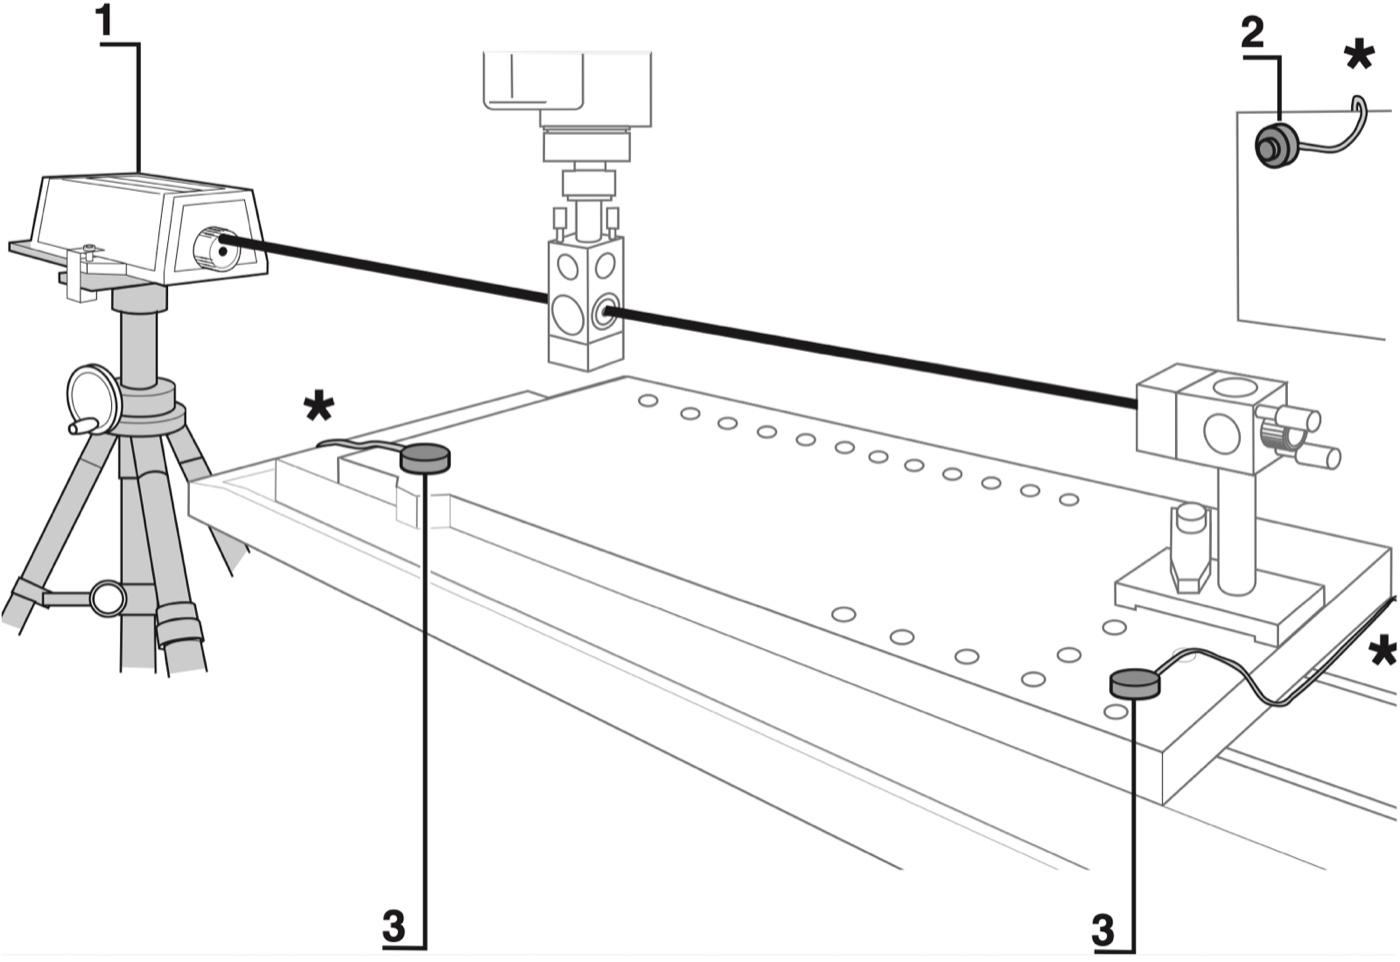
\includegraphics[keepaspectratio]{images/linearity-meas.jpg}}

}

\caption{Linearity measurement}

\end{figure}%

\subsection{Angle measurement}\label{angle-measurement}

\begin{itemize}
\tightlist
\item
  An angle interferometer only changes the optical paths difference upon
  rotation
\item
  Rotation can happen either on the splitter or in the retro-reflector
\item
  The action plane can be selected to measure the pitch or the yaw
  angles
\end{itemize}

\begin{figure}[H]

{\centering \pandocbounded{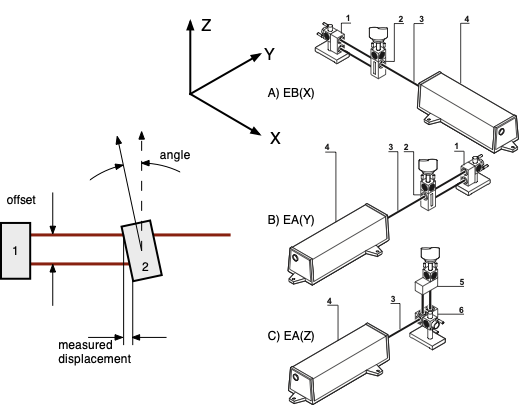
\includegraphics[keepaspectratio]{images-1/angle-meas.png}}

}

\caption{Angle measurement}

\end{figure}%

\subsection{Straightness measurement}\label{straightness-measurement}

A \href{https://en.wikipedia.org/wiki/Wollaston_prism}{Wollaston prism}
is a \textbf{beam-splitting prism} that splits a beam of light into two
beams with orthogonal polarizations. The two beams are
\textbf{diverging} at a small angle (typically 15--30 arcmin). The prism
is used to measure the straightness of an axis by measuring the lateral
displacement of the reflected beam.

\begin{center}
\includegraphics[width=\linewidth,height=4.16667in,keepaspectratio]{1-machine_tools_files/mediabag/images-1/straightness-prism.pdf}
\end{center}

\subsection{Straightness measurement}\label{straightness-measurement-1}

\begin{itemize}
\tightlist
\item
  By aligning the Wollaston prism action plane with XY and with XZ
  planes it is possible to measure the straightness of the X axis in Y
  and Z directions
\end{itemize}

\begin{figure}[H]

{\centering \pandocbounded{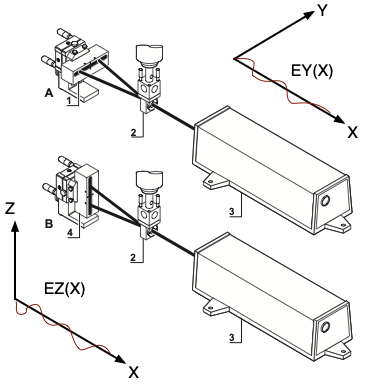
\includegraphics[keepaspectratio]{images-1/straightness-meas.png}}

}

\caption{Wollaston prism}

\end{figure}%

\subsection{Squareness measurement}\label{squareness-measurement}

\begin{itemize}
\tightlist
\item
  By combining lateral displacement measurement with an \textbf{optical
  square} it is possible to measure the squareness between two axes.
\item
  The optical square is a \textbf{reflecting prism} that reflects the
  laser beam at 90° its incoming direction
\end{itemize}

\begin{figure}[H]

{\centering \pandocbounded{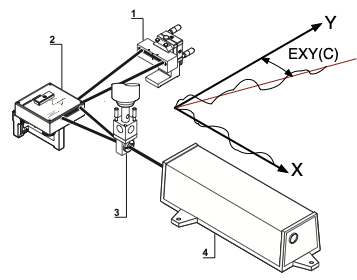
\includegraphics[keepaspectratio]{images-1/squareness-meas.png}}

}

\caption{Wollaston prism and optical square}

\end{figure}%

\subsection{}\label{section-4}

\subsection{Calibration}\label{calibration}

\subsection{Laser interferometer: three-axis machine tool
installation}\label{laser-interferometer-three-axis-machine-tool-installation}

High precision machine tools are equipped with a laser interferometer to
measure the actual position of the axes.

\begin{itemize}
\tightlist
\item
  one laser head (emitter only)
\item
  one receiver per axis
\item
  beam splitters direct 1/3 of the total source power to each axis
\end{itemize}

\begin{tcolorbox}[enhanced jigsaw, arc=.35mm, bottomrule=.15mm, bottomtitle=1mm, breakable, colback=white, colbacktitle=quarto-callout-note-color!10!white, colframe=quarto-callout-note-color-frame, coltitle=black, left=2mm, leftrule=.75mm, opacityback=0, opacitybacktitle=0.6, rightrule=.15mm, title=\textcolor{quarto-callout-note-color}{\faInfo}\hspace{0.5em}{Note}, titlerule=0mm, toprule=.15mm, toptitle=1mm]

Laser beam can be affected by refraction index changes and by air
turbulence, so the machine is usually equipped with a
\textbf{temperature and pressure sensor} to correct the measured
distance and the laser is usually enclosed in a \textbf{protective tube}
to avoid air turbulence.

\end{tcolorbox}

\begin{figure}[H]

{\centering 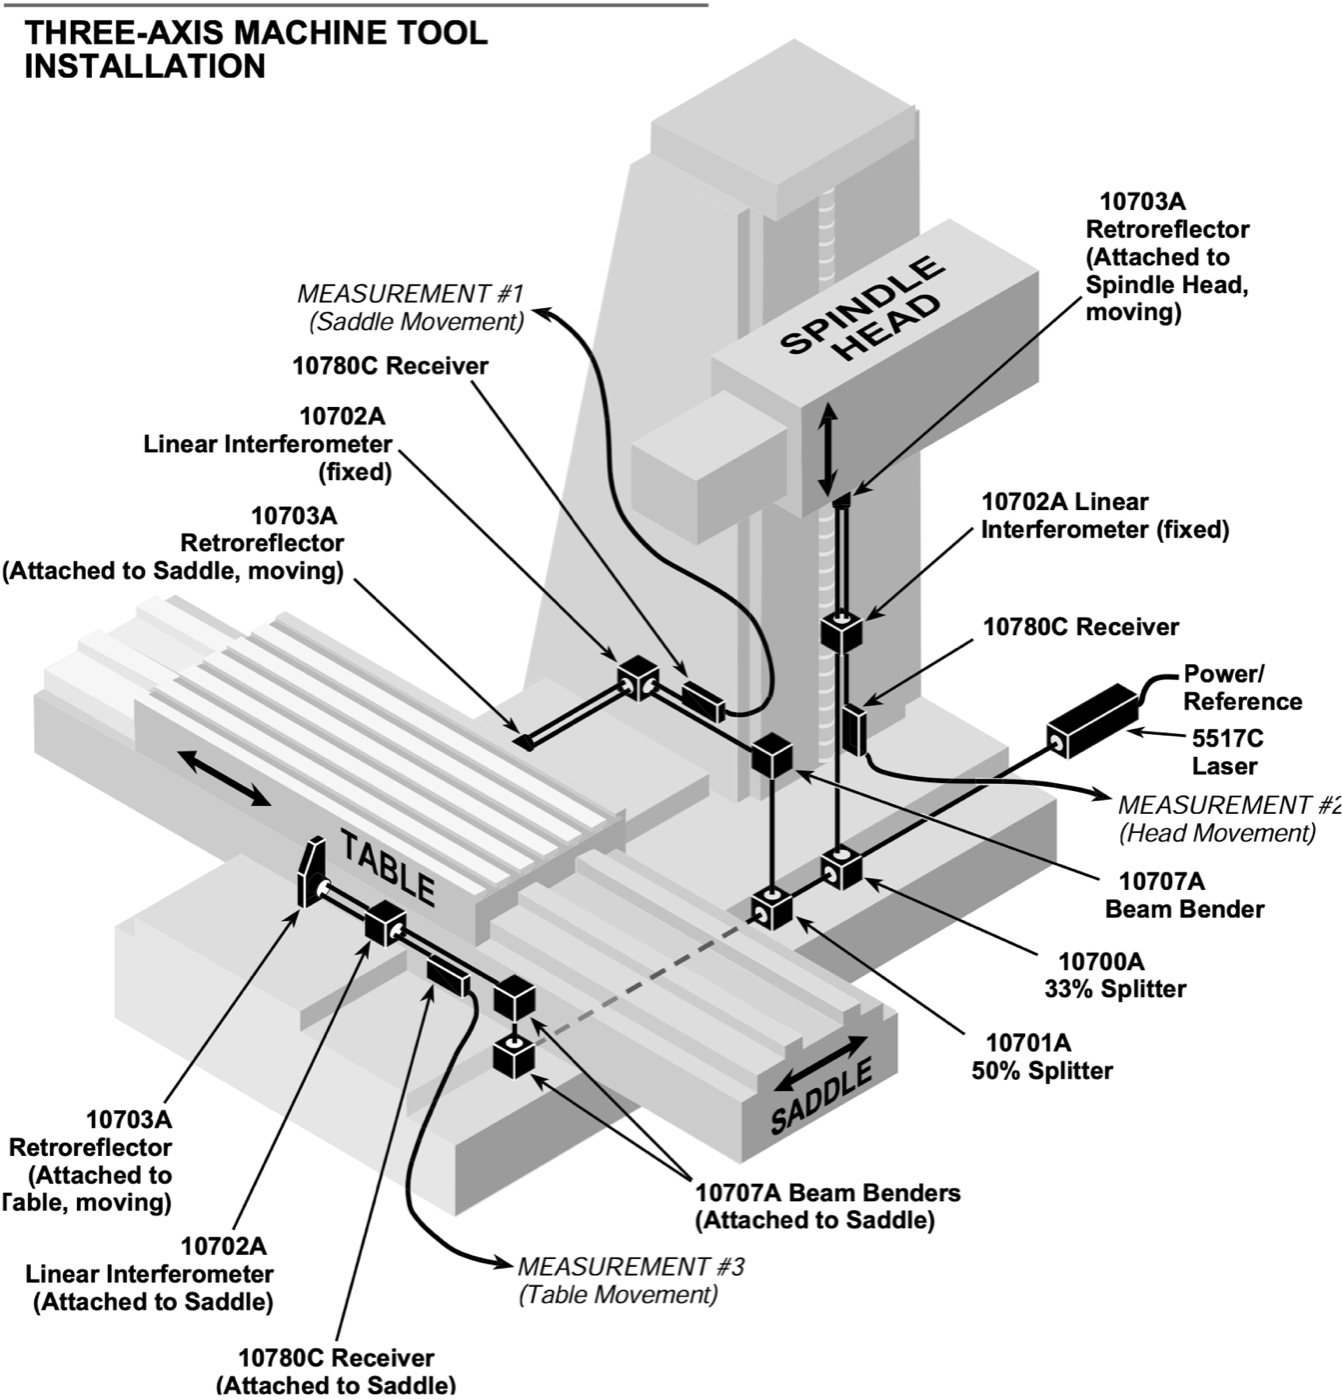
\includegraphics[width=\linewidth,height=4.89583in,keepaspectratio]{images/three-axis.jpg}

}

\caption{Using \textbf{LIF} as measurement tool}

\end{figure}%




\end{document}
